\documentclass[11pt,twoside,openany]{book}
\usepackage{estilo}
\renewcommand{\cabecalhocapitulo}{Cap.~II — Conjuntos}

\title{Conjuntos}
\begin{document}
\frontmatter
\begin{titlepage}
  \centering\sffamily
  \vspace*{5cm}
  {\color{cinza}\large Fundamentos de Matemática Elementar · vol.~1\par}
  \vspace{1.2em}
  {\color{acento}\Huge\bfseries Capítulo II\par\vspace{0.3em}Conjuntos\par}
  \vspace{2em}
  {\large Material didático\par}
  \vfill
  {\small\color{cinza}Didática v4 · novembro de 2026\par}
\end{titlepage}
\tableofcontents

\mainmatter
\setcounter{chapter}{1}
\chapter{Conjuntos}
% ============================================================
% Abertura geral do capítulo — escrita no FECHAMENTO (etapa 5), quando todas as unidades existem.
% Seções: por que este capítulo · linha do tempo · mapa das unidades · notação · como usar.
% Referência pronta: capitulos/v1c1-nocoes-de-logica/tex/abertura.tex
% ============================================================
\section*{Abertura do capítulo}
\addcontentsline{toc}{section}{Abertura do capítulo}
\markright{Abertura do capítulo}

\subsection*{Por que este capítulo}
% 2–4 parágrafos: o que o capítulo dá ao estudante, onde ele será usado nos capítulos seguintes,
% e a pergunta que o atravessa. Sem afirmação de frequência sem fonte (E-R3-5).
«A escrever no fechamento.»

\subsection*{Linha do tempo}
% Só marcos contados em alguma unidade (narrativa ou observação). Cada linha com \src e a unidade.
Os marcos abaixo são os que o capítulo usa; cada um é contado, com suas fontes, na unidade indicada.
{\small
\renewcommand{\arraystretch}{1.12}
\begin{longtable}{>{\raggedleft\arraybackslash}p{1.9cm}>{\raggedright\arraybackslash}p{10.6cm}c}\toprule
\textbf{quando} & \textbf{o quê} & \textbf{unid.}\\\midrule\endfirsthead
\toprule\textbf{quando} & \textbf{o quê} & \textbf{unid.}\\\midrule\endhead
\bottomrule\endfoot
--- & «marco»\src{fme} & ---\\
\end{longtable}}

\subsection*{Mapa das unidades}
% Diagrama de pré-requisitos (TikZ) + tabela "a pergunta que a unidade responde" — igual à pergunta
% aberta de cada prefácio — e "o que você leva dela".
«Diagrama e tabela no fechamento.»

\subsection*{Tabela de notação}
% Símbolos do capítulo: lê-se · quem introduziu · quando · unidade. Só com fonte; sem fonte, "---".
«Tabela no fechamento.»

\subsection*{Como usar este material}
\textbf{A ordem de cada unidade.} Toda unidade segue a mesma sequência, e cada seção responde a uma pergunta: o \emph{Prefácio}, \enquote{por que isso merece ser estudado?}; \emph{De onde vem?}, \enquote{por que foi necessário, como surgiu e como o reconstruímos hoje?}; \emph{Onde é usado?}, \enquote{como reconheço uma situação em que devo usar isso?}; \emph{Erros comuns}, \enquote{onde o raciocínio costuma quebrar?}; \emph{Observações}, aprofundamentos opcionais; \emph{Exemplos} resolvidos e \emph{Questões}; a \emph{Síntese de domínio}, um teste do que você entendeu; e as \emph{Respostas}. As três primeiras seções formam um texto corrido, que pode ser lido sozinho, como um artigo. O que é fixo é a função de cada seção, não o tamanho. O glossário, no fim do capítulo, reúne os termos e símbolos de todas as unidades, para consulta.

\textbf{As caixas.} \emph{O mínimo que você precisa} (moldura azul) lembra os pré-requisitos. \emph{Construção} (amarela) mostra um conceito sendo montado passo a passo. \emph{Definição} (moldura azul) dá o enunciado formal. \emph{Para lembrar} (fundo azul-claro) resume a unidade numa frase e em poucos passos. \emph{Erros} (vermelho) seguem sempre o mesmo roteiro: o erro; por que ele parece plausível; onde o raciocínio quebra, com um contraexemplo concreto; como detectá-lo depois de escrever; como corrigi-lo; e onde ele aparece nos exemplos e questões. Em \emph{Onde é usado?}, as caixas de \emph{Mapa do problema} mostram como sair do enunciado para a ferramenta. \emph{Observações} (cinza, com o selo \opcional{} e letra menor) ampliam o conceito sem serem necessárias para usá-lo. A \emph{Síntese de domínio} (amarela) fecha a unidade: você responde, com suas palavras, o que o conceito significa, como foi construído, quando usá-lo e como não errar, e confere com a caixa \emph{Para lembrar}.

\textbf{Os níveis.} Exemplos e questões têm um selo de nível, que indica a \emph{função} do item, e não só a dificuldade. \nivel{1} é \emph{reconhecimento e aplicação}: a ferramenta está clara, e você a aplica. \nivel{2} é \emph{seleção e combinação}: é preciso perceber qual ferramenta usar e, às vezes, combinar mais de uma. \nivel{3} é \emph{transferência}: a ferramenta aparece numa situação diferente da que a teoria apresentou, e nenhum N3 está resolvido no texto. Dentro de cada nível, as questões vão da mais guiada para a menos guiada. As questões marcadas com \integradora{} misturam o assunto da unidade com outro, mas só entram se o assunto da unidade for necessário para resolvê-las.

\textbf{As etiquetas de procedência.} Cada exemplo e cada questão indicam de onde vêm:
\begin{itemize}[leftmargin=1.4em,itemsep=1pt]
  \item \textbf{prova com ano}, como [FUVEST 2019, 1ª fase, q.~12]: questão real, com o texto conferido na prova;
  \item \textbf{[\ldots\ via FME]}: questão real cujo texto foi tirado do próprio FME;
  \item \textbf{[FME, exercício $n$]}: exercício do livro-base; \textbf{[adaptado do FME, item $n$]}: exemplo da teoria do livro, reescrito para esta didática;
  \item \textbf{[adaptada de\ldots]}: questão de vestibular ou de concurso cujo texto original não pôde ser conferido na íntegra; foi reescrita, com a resposta conferida;
  \item \textbf{[histórico]}: problema ou experimento da história contada na unidade;
  \item \textbf{[autoral]}: escrita para este material.
\end{itemize}

\textbf{As fontes.} Os números sobrescritos, como este\src{fme}, remetem à lista de \emph{Fontes} no fim do capítulo. Histórias cuja veracidade não se pode verificar trazem a marca\anedota.

\textbf{Os identificadores.} As marcas cinza entre $\langle\ \rangle$, como \cobre{2-U3}, ligam o texto à matriz de cobertura: o número é a unidade, e a letra diz o tipo — \textbf{H} para uma construção (seção \emph{De onde vem?}), \textbf{U} para um contexto de uso, \textbf{E} para um erro comum, \textbf{O} para uma observação. Na primeira leitura, podem ser ignorados.

\textbf{As respostas.} As respostas trazem só o resultado final, no formato [\,14.\ (c)\,] ou [\,28.\ $5\sqrt3$\,]. Nas questões de demonstração, a resposta diz, em uma linha, \emph{o que a prova deve mostrar}. As respostas que podem ser obtidas por cálculo foram conferidas por um programa, separado da redação.
\clearpage

% %% UNIDADES (esqueleto.py acrescenta aqui) %%
% ============================================================
% Unidade 1 — Conjunto, elemento e descrição   (didática v3 · kit/didatica.md §2)
% Parte A, o "artigo": Prefácio, De onde vem?, Onde é usado?
% IDs: 1-H1..H4 · 1-U1..U3 · 1-E1..E4 · 1-O1, 1-O2 (matriz.yaml) · fonte única: dossies/u1.md
% ============================================================
\clearpage
\section{Conjunto, elemento e descrição}

% ------------------------------------------------------------
\Prefacio
\begin{prefacio}
\gancho{O 9 está ou não está na lista?}

Dois colegas leem no quadro: \enquote{os números $3, 5, 7, \ldots$}. Um deles jura que o 9 está ali; o outro, que não está. Os dois têm razão: o primeiro leu \enquote{os ímpares a partir de 3}; o segundo, \enquote{os primos ímpares}, e depois do 7 vem o 11. As reticências não disseram o bastante.

Outra situação. \enquote{Quais números satisfazem $x^2=2$?} Se procuramos entre as frações, nenhum; se procuramos entre todos os números reais, dois: $\sqrt2$ e $-\sqrt2$. A condição é a mesma; as respostas são diferentes, porque a pergunta não disse \emph{onde} procurar.

Toda a matemática deste capítulo fala de coleções: o conjunto das soluções de uma equação, o conjunto dos pontos de uma figura, os grupos de pessoas de uma pesquisa. Se a descrição de uma coleção deixa dúvida sobre quem pertence a ela, tudo o que vem depois herda a dúvida.

\textbf{Como descrever um conjunto de modo que ninguém possa discordar sobre quem está dentro e quem está fora?} É a pergunta desta unidade.

\textbf{Ao final, você será capaz de:} ler e escrever $\in$ e $\notin$; passar de uma lista de elementos a uma propriedade e de uma propriedade à lista; dizer, antes de resolver, em que universo se procuram as respostas; reconhecer conjuntos vazios e unitários; recusar uma \enquote{descrição} que não decide quem pertence.

\textbf{Pré-requisitos:} do Capítulo I, sentenças abertas e proposições logicamente falsas; do ensino fundamental, resolver equações do 1º e do 2º grau (usadas nas questões integradoras). O essencial está na caixa abaixo.
\end{prefacio}

\begin{minimo}
\begin{itemize}[leftmargin=1.4em,itemsep=1pt]
  \item \textbf{Sentença aberta.} \enquote{$x+1=4$} não é verdadeira nem falsa até que $x$ receba um valor; com $x=3$, vira uma proposição verdadeira (Cap.~I, Unidade~5).
  \item \textbf{Contradição.} Uma sentença da forma \enquote{$p$ e não $p$}, como \enquote{$x=1$ e $x\neq1$}, é falsa para todo valor de $x$ (Cap.~I, Unidade~4).
  \item \textbf{Os conjuntos numéricos, por enquanto informalmente.} $\mathbb{N}=\{0,1,2,3,\ldots\}$ (neste material, o 0 é natural); $\mathbb{Z}$: os inteiros; $\mathbb{Q}$: os números que se escrevem como fração de inteiros; $\mathbb{R}$: os reais, como $\sqrt2$ e $\pi$. O Capítulo III os define com cuidado.
\end{itemize}
\end{minimo}

% ------------------------------------------------------------
\DeOndeVem

\subsubsection{Por que alguém precisou disso}
Muitas vezes precisamos tratar uma coleção inteira — todos os números pares, todos os pontos que ficam à mesma distância de dois pontos $A$ e $B$ — como \emph{um único objeto matemático} e fazer perguntas sobre ela: quantos elementos ela tem? O 8 pertence a ela? Ela é igual a outra coleção? Para que essas perguntas tenham uma única resposta certa, a coleção precisa ficar determinada apenas por quais objetos pertencem a ela, de um modo que qualquer pessoa decida da mesma forma.

Tratar uma coleção como um objeto é uma ideia mais recente do que parece. Em 1872, estudando séries trigonométricas, o matemático Georg Cantor precisou lidar com conjuntos de pontos da reta. A cada conjunto de pontos ele associou um conjunto novo — o dos seus \emph{pontos-limite}, isto é, os pontos que têm, tão perto quanto se queira, outros pontos do conjunto — e passou a repetir essa operação sobre o resultado, como se repete uma conta.\src{sepEarly} Para fazer isso, Cantor tinha de tratar cada conjunto de pontos como uma coisa só, sobre a qual se opera, do mesmo modo que se opera com o número 3. Esse é o passo que a teoria dos conjuntos tornou comum.\src{sepEarly}

\begin{construcao}[conjunto e pertinência]{1-H1}
\begin{enumerate}[label=(\arabic*)]
  \item Queremos tratar uma coleção como um objeto.
  \item A única coisa que precisamos saber sobre ela é: dado um objeto $x$, ele \textbf{pertence} à coleção ($x\in A$) ou \textbf{não pertence} ($x\notin A$) — uma das duas, e não as duas (os princípios do Capítulo I).
  \item Então o conjunto fica determinado por quem pertence a ele. Não o definimos a partir de nada mais simples: \emph{conjunto}, \emph{elemento} e \emph{pertinência} são \textbf{noções primitivas}, aceitas sem definição.\src{fme}
  \item Como o conjunto é um objeto, ele pode ser elemento de outro conjunto. O conjunto das seleções de um campeonato mundial de futebol tem como elementos as seleções, e cada seleção é, por sua vez, um conjunto de jogadores.\src{fme}
\end{enumerate}
Indicamos conjuntos por letras maiúsculas ($A$, $B$, \ldots) e elementos por minúsculas ($a$, $x$, \ldots). No \textbf{diagrama de Euler-Venn}, o conjunto é a região limitada por uma linha fechada: os pontos de dentro são os elementos.
\begin{center}
\begin{tikzpicture}[scale=0.85]
\draw[acento,thick,fill=acentoclaro] (0,0) ellipse (1.6 and 0.95);
\node at (1.55,0.95) {$A$};
\fill (-0.6,0.25) circle (1.5pt) node[above]{$a$};
\fill (0.5,0.35) circle (1.5pt) node[above]{$b$};
\fill (-0.1,-0.4) circle (1.5pt) node[below]{$c$};
\fill (2.3,-0.6) circle (1.5pt) node[right]{$d$};
\node[right] at (3.2,0) {$a\in A,\ b\in A,\ c\in A,\ d\notin A$};
\end{tikzpicture}
\end{center}
\end{construcao}

\subsubsection{Duas maneiras de dizer quem pertence}
Há duas maneiras naturais de fixar um conjunto: listar os elementos ou dar uma condição que eles, e só eles, satisfazem.

\begin{construcao}[enumeração e propriedade]{1-H2}
\begin{enumerate}[label=(\arabic*)]
  \item \textbf{Enumeração.} Escrevemos os elementos entre chaves: o conjunto das vogais é $\{a, e, i, o, u\}$. Se o conjunto é infinito, ou finito e muito grande, escrevemos os primeiros elementos e reticências — \emph{desde que a lei de formação fique visível}: $\{1, 3, 5, 7, 9, \ldots\}$; $\{0, 1, 2, \ldots, 500\}$.\src{fme}
  \item \textbf{Propriedade característica.} Escrevemos $A=\{x\mid x \text{ tem a propriedade } P\}$ e lemos \enquote{$A$ é o conjunto dos $x$ tais que $x$ tem a propriedade $P$}. Por exemplo, $\{x\mid x\text{ é divisor inteiro de }3\}=\{1,-1,3,-3\}$.\src{fme} Quando os elementos são valores de uma expressão, também se escreve a expressão antes da barra: $\{2^n\mid n\in\mathbb{N}\}=\{1,2,4,8,\ldots\}$ (lê-se \enquote{o conjunto dos $2^n$, com $n$ natural}).
  \item \textbf{Passar de uma para a outra.} Da propriedade para a lista: testar candidatos. Da lista para a propriedade: achar algo que os listados têm em comum e que mais ninguém tem.
  \item \textbf{A lista com reticências é uma propriedade disfarçada.} Quem escreve \enquote{\ldots} supõe que o leitor vai adivinhar a mesma lei. Se duas leis diferentes começam igual, a lista não fixou o conjunto (erro 1-E2).
\end{enumerate}
\end{construcao}

A propriedade parece resolver tudo: diga a condição, e o conjunto está dado. A próxima história mostra que, sozinha, ela não basta.

\subsubsection{Quando a propriedade sozinha falha}
O lógico alemão Gottlob Frege tentou dar à aritmética um fundamento puramente lógico.\src{sepRussell} Uma das peças do seu sistema era a possibilidade de, a partir de qualquer conceito, passar à sua \emph{extensão} — a coleção dos objetos que caem sob aquele conceito.\src{sepZermelo}\src{frege1903} Lido hoje, é o que se chama \textbf{princípio de compreensão}: para toda condição $P(x)$, existe o conjunto $\{x\mid P(x)\}$.\src{sepRussell}

Em 1901, Bertrand Russell encontrou uma contradição ao pensar na classe de todas as classes que não são membros de si mesmas; em 16 de junho de 1902, escreveu a Frege mostrando que ela atingia o sistema de Frege.\src{sepRussell}\src{vanH} Em notação moderna, é o conjunto
\[
R=\{x\mid x\notin x\}.
\]
Pergunte se $R$ pertence a $R$. Se $R\in R$, então $R$ satisfaz a condição \enquote{$x\notin x$}, isto é, $R\notin R$. Se $R\notin R$, então $R$ satisfaz a condição, e portanto $R\in R$. Cada possibilidade leva à sua negação; portanto, a condição \enquote{$x\notin x$} não define conjunto nenhum. A carta chegou quando o segundo volume da obra de Frege estava indo para a gráfica; no apêndice, o próprio Frege pergunta se é sempre permitido falar da extensão de um conceito e, se não for, como reconhecer as exceções.\src{sepZermelo}

A saída que a matemática adotou foi proposta em 1908 pelo matemático Ernst Zermelo. Ele escreveu que era preciso abandonar a suposição de que a toda noção logicamente definível corresponde um conjunto, e propôs, no lugar dela, um axioma de \emph{separação}: dado um conjunto já existente e uma propriedade sem ambiguidade, pode-se \emph{separar} dele o conjunto dos elementos que têm a propriedade.\src{sepZermelo}\src{zermelo1908} Lido hoje, o axioma garante os conjuntos da forma $\{x\in S\mid P(x)\}$. Com a condição \enquote{$x\notin x$}, o conjunto $\{x\in S\mid x\notin x\}$ só contém elementos de $S$; o argumento de Russell, refeito, mostra apenas que esse conjunto não é elemento de $S$ — nenhuma contradição.\src{sepRussell} A convenção que você vai usar em todo o curso é a forma escolar dessa ideia: ao descrever um conjunto por uma propriedade, fixe antes o conjunto de onde vêm os candidatos.\src{fme}

\begin{construcao}[o conjunto universo]{1-H3}
\begin{enumerate}[label=(\arabic*)]
  \item Pergunta: \emph{qual é o conjunto dos pontos $P$ que ficam à mesma distância de dois pontos dados $A$ e $B$, com $A\neq B$?}\src{fme} A resposta depende de onde os pontos podem estar:
\begin{itemize}[leftmargin=1.2em,itemsep=0pt]
  \item se os pontos estão na reta $AB$, o conjunto tem um único elemento: o ponto médio de $\overline{AB}$;
  \item se estão num plano que contém $A$ e $B$, o conjunto é a mediatriz do segmento $\overline{AB}$;
  \item se estão no espaço, é o plano mediador de $\overline{AB}$ (o plano perpendicular a $\overline{AB}$ pelo ponto médio).
\end{itemize}
A mesma propriedade, três conjuntos diferentes. Com números acontece o mesmo: $x^2=2$ não tem solução entre as frações e tem duas entre os reais.
  \item Logo, a propriedade precisa vir acompanhada do conjunto de onde vêm os candidatos. Esse conjunto se chama \textbf{conjunto universo}, $U$. Escrevemos
\[
A=\{x\in U\mid x \text{ tem a propriedade } P\}.
\]
  \item Além de tirar a ambiguidade, o universo evita a contradição de Russell: separar elementos de um conjunto já dado nunca produz um \enquote{conjunto} impossível.
  \item Convenção: ao descrever um conjunto por propriedade, \textbf{fixe o universo antes}. Se procuramos as soluções reais de uma equação, $U=\mathbb{R}$; se a solução de um problema tem de ser um número inteiro, $U=\mathbb{Z}$; num problema de Geometria Plana, $U$ é um plano.\src{fme}
\end{enumerate}
\end{construcao}

\begin{definicao}[conjunto universo]
O \textbf{conjunto universo} $U$ de um problema é o conjunto ao qual pertencem todos os elementos considerados nele. Descrever um conjunto por uma propriedade $P$ é escrever $\{x\in U\mid x\text{ tem }P\}$: os elementos de $U$ que satisfazem $P$, e só eles.
\end{definicao}

\subsubsection{Quantos elementos: nenhum, um, muitos}
\begin{construcao}[conjunto vazio e conjunto unitário]{1-H4}
\begin{enumerate}[label=(\arabic*)]
  \item Um conjunto pode ter um só elemento: o conjunto das soluções de $3x+1=10$ é $\{3\}$.\src{fme}
  \item Uma propriedade que \emph{nenhum} candidato satisfaz — seja falsa pela forma, como \enquote{$x=1$ e $x\neq1$}, seja falsa por um fato sobre os números, como \enquote{$x\neq x$} ou \enquote{$x>0$ e $x<0$} — dá um conjunto sem elemento algum.\src{fme} Como um conjunto é decidido por quem pertence, todos esses conjuntos sem elementos são o mesmo: o conjunto vazio, $\varnothing$.
  \item Cuidado com as chaves: $\{0\}$ \emph{não} é vazio — tem um elemento, o número 0. E $\{\varnothing\}$ também não: tem um elemento, o próprio conjunto vazio. Pense numa caixa: $\varnothing$ é a caixa vazia; $\{\varnothing\}$ é uma caixa que contém uma caixa vazia.
  \item Ser vazio também depende do universo: $\{x\in\mathbb{Z}\mid 2x+1=0\}=\varnothing$, mas $\{x\in\mathbb{Q}\mid 2x+1=0\}=\{-\tfrac12\}$.
  \item Além de vazios e unitários, falaremos de conjuntos \textbf{finitos} (dá para listar todos os elementos, e a lista acaba) e \textbf{infinitos} (a lista nunca acaba, como em $\mathbb{N}$). Por enquanto, essa ideia informal basta.
\end{enumerate}
\end{construcao}

\begin{definicao}[conjunto unitário e conjunto vazio]
\textbf{Conjunto unitário} é o que possui um único elemento. \textbf{Conjunto vazio}, indicado por $\varnothing$, é o que não possui elemento algum.
\end{definicao}

\begin{paralembrar}\label{lembrar-u1}
\textbf{Um conjunto é decidido por quem pertence a ele: descreva-o por uma lista com lei visível ou por uma propriedade dentro de um universo.}
\begin{enumerate}[label=\arabic*.,leftmargin=1.4em,itemsep=1pt]
  \item Fixe o universo $U$ de onde vêm os candidatos.
  \item Escreva a condição $P(x)$ sem ambiguidade: $\{x\in U\mid P(x)\}$.
  \item Teste: para cada candidato, dá para decidir se ele pertence? Se não dá, ainda não há conjunto.
\end{enumerate}
\end{paralembrar}

% ------------------------------------------------------------
\OndeEUsado

A linguagem de conjuntos aparece sempre que um enunciado pede \enquote{o conjunto de\ldots}, \enquote{as soluções de\ldots}, \enquote{os pontos tais que\ldots} — e também fora da matemática escolar, quando um programa filtra itens de uma coleção. Esta seção ensina a reconhecer o que o enunciado está pedindo. São quatro situações.

\subsubsection{Mapa do problema}

\begin{caso}{1 · \enquote{dê os elementos}, \enquote{descreva}}{1-U1}
\mapa{\enquote{dê os elementos}, \enquote{escreva com símbolos}, \enquote{descreva por meio de uma propriedade}}
{uma lista com lei visível, ou uma condição que os listados satisfazem e mais ninguém}
{1-H2: testar candidatos (propriedade $\to$ lista) ou achar o que é comum (lista $\to$ propriedade)}
\reconhecer O verbo do enunciado pede uma tradução: de lista para condição (\enquote{descreva por meio de uma propriedade}) ou de condição para lista (\enquote{dê os elementos}). Pode haver mais de uma propriedade certa; o que importa é que ela pegue todos os listados e nenhum outro. Treino: \exref{ex:u1:listar}; questões \ref{u1:listar} e \ref{u1:fme13}.
\end{caso}

\begin{caso}{2 · \enquote{qual é o conjunto dos\ldots?}}{1-U2}
\mapa{\enquote{qual é o conjunto dos\ldots}, \enquote{resolva}, \enquote{determine as soluções}, às vezes sem dizer onde}
{o universo: dito no enunciado (\enquote{em $\mathbb{Z}$}, \enquote{no plano}) ou implícito no contexto}
{1-H3: escrever $\{x\in U\mid P(x)\}$ antes de calcular}
\reconhecer O sinal é uma pergunta que descreve os elementos por uma condição sem dizer onde procurá-los, como a da construção 1-H3: \enquote{qual é o conjunto dos pontos que ficam à mesma distância de $A$ e de $B$?}. Sem o universo, essa pergunta tem três respostas. Quando o enunciado não diz o universo, procure-o no contexto: \enquote{número de alunos} está em $\mathbb{N}$; \enquote{solução real} está em $\mathbb{R}$. Treino: \exref{ex:u1:universo}; questões \ref{u1:equacao} e \ref{u1:distancia}.
\end{caso}

\begin{caso}{3 · um programa que filtra uma coleção}{1-U2}
\mapa{código que percorre uma coleção e guarda os itens que passam num teste}
{a coleção percorrida (o universo) e o teste (a propriedade)}
{1-H3 escrito em código: \texttt{\{x for x in U if P(x)\}}}
\reconhecer Na linguagem Python, um conjunto pode ser escrito quase como no caderno. O tutorial oficial traz o exemplo \texttt{\{x for x in 'abracadabra' if x not in 'abc'\}}, cujo resultado é o conjunto \texttt{\{'r', 'd'\}}.\src{pyTut} Leia: \enquote{o conjunto das letras $x$ da palavra \emph{abracadabra} tais que $x$ não é $a$, $b$ nem $c$}. O universo — a palavra percorrida — é obrigatório: o programa não tem como \enquote{procurar em tudo}. As letras repetidas entram uma vez só. Treino: \qref{u1:listar}, item (e).
\end{caso}

\begin{caso}{4 · \enquote{quais são vazios? quais são unitários?}}{1-U3}
\mapa{\enquote{quais dos conjuntos abaixo são vazios / unitários / finitos?}}
{quantos candidatos do universo satisfazem a propriedade}
{1-H4 junto com 1-H3: contar as soluções \emph{no universo dado}}
\reconhecer O enunciado apresenta vários conjuntos descritos por propriedades e pergunta quais são vazios, unitários ou finitos. Antes de contar, verifique duas coisas: em que universo se está (o mesmo intervalo pode ser vazio entre os inteiros e infinito entre os reais) e se a propriedade é falsa para todos (\enquote{$x-x=1$}) ou verdadeira para todos (\enquote{$x-x=0$}). Treino: \exref{ex:u1:classificar}; questões \ref{u1:vazios} e \ref{u1:unitarios}.
\end{caso}

\subsubsection{Tabela de gatilhos}
\begin{gatilhos}
\enquote{dê os elementos}, \enquote{descreva} & 1-H2 & testar candidatos ou achar o que é comum & \mbox{1-U1\,·\,q.\,\ref{u1:listar}}\\\fino
conjunto-solução sem universo explícito & 1-H3 & perguntar \enquote{procurando onde?} antes de calcular & \mbox{1-U2\,·\,q.\,\ref{u1:equacao}}\\\fino
figura descrita por uma distância & 1-H3 & reta, plano ou espaço mudam a resposta & \mbox{1-U2\,·\,q.\,\ref{u1:distancia}}\\\fino
lista com reticências & 1-H2 & a lei está visível? se não, escreva a propriedade & \mbox{1-U1\,·\,q.\,\ref{u1:reticencias}}\\\fino
\enquote{vazio? unitário?} & 1-H4 & contar quantos candidatos de $U$ satisfazem $P$ & \mbox{1-U3\,·\,q.\,\ref{u1:vazios}}\\\fino
palavra vaga (\enquote{grande}, \enquote{bom}, \enquote{perto}) & 1-H1 & existe critério de pertinência? & \mbox{1-E4\,·\,q.\,\ref{u1:criterio}}\\
\end{gatilhos}

% ============================================================
% Unidade 1 — Parte B: erros, observações, exemplos, questões, síntese, respostas
% Fonte única: dossies/u1.md · respostas conferidas em verif/u1.py
% ============================================================
\ErrosComuns

\begin{erro}{Esquecer o universo}{1-E1}
\campo{O erro.} Resolver $x^2=2$ e responder $\{-\sqrt2,\sqrt2\}$ quando o enunciado procurava entre as frações; ou responder $\{-2,3\}$ para $x^2-x-6=0$ quando o universo era $\mathbb{N}$, onde $-2$ não está.
\campo{Por que parece plausível.} A equação é a mesma; resolver \enquote{dá} as raízes, e o universo parece um detalhe do enunciado.
\campo{Onde quebra.} $\{x\in\mathbb{Q}\mid x^2=2\}=\varnothing$, mas $\{x\in\mathbb{R}\mid x^2=2\}=\{-\sqrt2,\sqrt2\}$. E $\{x\in\mathbb{Z}\mid 2x+1=0\}=\varnothing$, mas em $\mathbb{Q}$ o conjunto é $\{-\tfrac12\}$.
\campo{Como detectar.} Depois de escrever a resposta, confira cada elemento: ele pertence a $U$? E falta algum elemento de $U$ que satisfaz a condição?
\campo{Como corrigir.} Escreva o universo na primeira linha da resolução, $\{x\in U\mid\ldots\}$, e filtre as soluções no fim (construção 1-H3).
\campo{Onde aparece.} \exref{ex:u1:universo}; questões \ref{u1:unitarios} e \ref{u1:equacao}.
\end{erro}

\begin{erro}{Reticências sem lei clara}{1-E2}
\campo{O erro.} Escrever $\{1,2,4,\ldots\}$ ou $\{3,5,7,\ldots\}$ e supor que todo leitor vai continuar do mesmo jeito.
\campo{Por que parece plausível.} Quem escreveu já tinha uma lei na cabeça; para ele, \enquote{o padrão é óbvio}.
\campo{Onde quebra.} Em $\{1,2,4,\ldots\}$, dobrando, o próximo é 8; somando 1, depois 2, depois 3, o próximo é 7. Em $\{3,5,7,\ldots\}$, os ímpares a partir de 3 contêm o 9; os primos ímpares, não.
\campo{Como detectar.} Tente escrever duas leis diferentes que comecem com os mesmos termos. Se conseguir, a lista não fixou o conjunto.
\campo{Como corrigir.} Liste termos suficientes para eliminar as outras leis ou, melhor, troque a lista pela propriedade (construção 1-H2).
\campo{Onde aparece.} \exref{ex:u1:reticencias}; \qref{u1:reticencias}.
\end{erro}

\begin{erro}{Confundir $\varnothing$ com $\{0\}$ ou com $\{\varnothing\}$}{1-E3}
\campo{O erro.} Dizer que $\{0\}$ é vazio (\enquote{só tem zero}), que $\{\varnothing\}$ é vazio, ou que $\{x\mid x-x=0\}$ é vazio.
\campo{Por que parece plausível.} \enquote{Zero} e \enquote{vazio} lembram \enquote{nada}; e $x-x=0$ \enquote{dá zero}.
\campo{Onde quebra.} $\{0\}$ tem um elemento, o número 0; $\{\varnothing\}$ tem um elemento, o conjunto vazio. E $x-x=0$ é verdadeira para \emph{todo} $x$: $\{x\in U\mid x-x=0\}=U$. Vazio é $\{x\in U\mid x-x=1\}$.
\campo{Como detectar.} Conte os objetos entre as chaves. Para uma propriedade, pergunte: existe algum candidato que a satisfaz?
\campo{Como corrigir.} $\varnothing$ é o único conjunto sem elementos; qualquer coisa escrita entre as chaves já é um elemento (construção 1-H4).
\campo{Onde aparece.} \exref{ex:u1:vazio}; questões \ref{u1:quantos} e \ref{u1:vazios}.
\end{erro}

\begin{erro}{Aceitar uma descrição sem critério de pertinência}{1-E4}
\campo{O erro.} Tratar \enquote{os números grandes}, \enquote{os bons alunos} ou \enquote{as cidades perto do mar} como conjuntos.
\campo{Por que parece plausível.} Na conversa, todo mundo entende mais ou menos o que se quer dizer.
\campo{Onde quebra.} O número $10^6$ é grande? E $10^3$? Cada leitor decide de um jeito, e não há como responder \enquote{$x\in A$?} para todo $x$. Já \enquote{os naturais menores que $10^{100}$} é um conjunto: enorme, mas decidido.
\campo{Como detectar.} Escolha um candidato de fronteira e pergunte se ele pertence. Se a resposta depende de opinião, não há conjunto.
\campo{Como corrigir.} Troque a palavra vaga por uma condição decidível: \enquote{média maior ou igual a 7}, \enquote{a menos de 50 km do litoral} (construção 1-H1 e caixa \emph{Para lembrar}).
\campo{Onde aparece.} \exref{ex:u1:classificar}; \qref{u1:criterio}.
\end{erro}

% ------------------------------------------------------------
\Observacoes

\begin{obs}{1-O1}
\textbf{O conjunto como objeto.} Para os pioneiros, não era óbvio que uma coleção infinita, como $\mathbb{N}$, pudesse ser tratada como uma coisa só, sobre a qual se opera, do mesmo modo que o número 3. O historiador José Ferreirós aponta essa \enquote{objetidade} como o elemento novo da teoria dos conjuntos: as ideias de coleção e de classe são muito antigas; o que mudou foi tratar o conjunto como um objeto matemático.\src{sepEarly}
\end{obs}

\begin{obs}{1-O2}
\textbf{Não existe \enquote{o conjunto de tudo}.} O axioma de separação tem uma consequência curiosa. Dado qualquer conjunto $S$, o conjunto $\{x\in S\mid x\notin x\}$ não pode ser elemento de $S$ (é o argumento de Russell, agora sem contradição). Portanto, nenhum conjunto contém todos os objetos: Zermelo concluiu, em 1908, que o domínio de todos os objetos não é, ele próprio, um conjunto.\src{sepZermelo}\src{zermelo1908} É por isso que o universo $U$ de um problema é sempre \enquote{um universo}, escolhido para aquele assunto, e nunca \enquote{o universo de tudo}.
\end{obs}

% ------------------------------------------------------------
\Exemplos

\begin{exemplo}{}{1}{adaptado do FME, exercícios 11 e 12}{1-H1, 1-H2, 1-U1}
\label{ex:u1:listar}
\begin{enumerate}[label=\alph*)]
  \item Dê os elementos de $A=\{x\mid x\text{ é letra da palavra \emph{matemática}}\}$ e de $B=\{x\mid x\text{ é cor da bandeira brasileira}\}$.
  \item Descreva por uma propriedade característica $C=\{0,2,4,6,8,\ldots\}$ e $D=\{0,1,2,\ldots,9\}$.
\end{enumerate}
\plano Em (a), percorrer os candidatos (as letras da palavra, as cores da bandeira) e guardar cada um uma vez. Em (b), achar o que os listados têm em comum e mais ninguém tem.
\resolucao (a) $A=\{m,a,t,e,i,c\}$ e $B=\{\text{verde},\text{amarelo},\text{azul},\text{branco}\}$. (b) $C=\{x\in\mathbb{N}\mid x\text{ é par}\}$ e $D=\{x\in\mathbb{N}\mid x\le 9\}$ (os algarismos).
\comentario A palavra \emph{matemática} tem dez letras, mas $A$ tem seis elementos: a letra \emph{a} aparece três vezes na palavra, e \emph{m} e \emph{t} aparecem duas vezes cada; no conjunto, cada uma entra uma vez só, porque o conjunto registra apenas \emph{se} a letra pertence (a Unidade~2 volta a isso). Em (b), \enquote{par} sozinho não bastaria para $C$: os pares negativos ficariam dentro; o universo $\mathbb{N}$ faz o trabalho.
\end{exemplo}

\begin{exemplo}{}{1}{autoral}{1-H1, 1-H4, 1-E3}
\label{ex:u1:vazio}
Quantos elementos têm $\varnothing$, $\{0\}$, $\{\varnothing\}$ e $\{x\in\mathbb{R}\mid x\neq x\}$?
\plano Contar o que está entre as chaves; para a propriedade, procurar algum real que a satisfaça.
\resolucao $\varnothing$ não tem elementos: 0. $\{0\}$ tem um elemento, o número 0: 1. $\{\varnothing\}$ tem um elemento, o conjunto vazio: 1. Nenhum real é diferente de si mesmo, então $\{x\in\mathbb{R}\mid x\neq x\}=\varnothing$: 0.
\comentario Os quatro números são 0, 1, 1, 0. O erro 1-E3 está em achar que $\{0\}$ ou $\{\varnothing\}$ são vazios: os dois têm um elemento, e o fato de um conjunto poder ser elemento de outro (construção 1-H1) é o que torna $\{\varnothing\}$ diferente de $\varnothing$.
\end{exemplo}

\begin{exemplo}{}{2}{autoral}{1-H3, 1-U2, 1-E1}
\label{ex:u1:universo}
Determine $\{x\in U\mid x^2-2=0\}$ para $U=\mathbb{Q}$ e para $U=\mathbb{R}$; e $\{x\in U\mid 2x+1=0\}$ para $U=\mathbb{Z}$ e para $U=\mathbb{Q}$.
\plano Resolver cada equação uma vez, como se não houvesse universo, e depois guardar só as soluções que estão em $U$.
\resolucao As soluções de $x^2=2$ são $\sqrt2$ e $-\sqrt2$, que não são frações. Logo $\{x\in\mathbb{Q}\mid x^2-2=0\}=\varnothing$ e $\{x\in\mathbb{R}\mid x^2-2=0\}=\{-\sqrt2,\sqrt2\}$. A solução de $2x+1=0$ é $-\tfrac12$, que não é inteiro: $\{x\in\mathbb{Z}\mid 2x+1=0\}=\varnothing$ e $\{x\in\mathbb{Q}\mid 2x+1=0\}=\{-\tfrac12\}$.
\comentario A mesma condição deu conjuntos diferentes. Por isso a construção 1-H3 manda fixar $U$ antes de resolver, e o teste do erro 1-E1 é conferir, no fim, se cada elemento pertence a $U$.
\end{exemplo}

\begin{exemplo}{}{2}{autoral}{1-H2, 1-U1, 1-E2}
\label{ex:u1:reticencias}
Encontre duas leis diferentes para a lista $\{1,2,4,\ldots\}$, escreva cada conjunto por uma propriedade e diga qual número viria depois do 4 em cada caso.
\plano Procurar leis que produzam 1, 2, 4 e depois se separem; escrever cada uma na forma \enquote{expressão $\mid$ condição}.
\resolucao Primeira lei: cada termo é o dobro do anterior; o conjunto é $\{2^n\mid n\in\mathbb{N}\}=\{1,2,4,8,16,\ldots\}$, e depois do 4 vem o 8. Segunda lei: soma-se 1, depois 2, depois 3, e assim por diante; o termo de ordem $n$ (contando de $n=0$) é $1+\tfrac{n(n+1)}{2}$, e o conjunto é $\{1+\tfrac{n(n+1)}{2}\mid n\in\mathbb{N}\}=\{1,2,4,7,11,\ldots\}$, em que depois do 4 vem o 7.
\comentario Os dois conjuntos começam iguais e são diferentes: o 7 está em um e não no outro. A lista $\{1,2,4,\ldots\}$ não fixou nenhum dos dois (erro 1-E2). A propriedade fixou.
\end{exemplo}

\begin{exemplo}{}{2}{autoral}{1-H4, 1-U3, 1-E4}
\label{ex:u1:classificar}
Classifique como vazio, unitário, finito com mais de um elemento ou infinito, ou diga que a descrição não define conjunto:
\begin{multicols}{2}
\begin{enumerate}[label=\alph*)]
  \item $\{x\in\mathbb{N}\mid x<0\}$
  \item $\{x\in\mathbb{Z}\mid x^2=9\text{ e }x>0\}$
  \item $\{x\in\mathbb{Z}\mid 3<x<4\}$
  \item $\{x\in\mathbb{R}\mid 3<x<4\}$
  \item os números grandes
\end{enumerate}
\end{multicols}
\plano Para cada item, ver quantos candidatos do universo satisfazem a condição; para (e), procurar um critério de pertinência.
\resolucao (a) Nenhum natural é negativo: vazio. (b) $x^2=9$ dá $x=3$ ou $x=-3$; com $x>0$, sobra $\{3\}$: unitário. (c) Não há inteiro entre 3 e 4: vazio. (d) Há infinitos reais entre 3 e 4 ($3{,}1$; $3{,}01$; $3{,}001$; \ldots): infinito. (e) Não há como decidir se $1000$ é \enquote{grande}: não define conjunto.
\comentario Compare (c) e (d): a mesma condição, vazio num universo e infinito no outro. Em (e), o problema não é o tamanho, e sim a falta de critério (erro 1-E4).
\end{exemplo}

\begin{exemplo}{}{3}{autoral}{1-H3}
\label{ex:u1:barbeiro}
Numa vila, há um barbeiro, homem e morador da vila, que barbeia exatamente os homens da vila que não se barbeiam a si mesmos. O barbeiro se barbeia?
\plano Testar as duas possibilidades contra a regra que descreve o barbeiro.
\resolucao Se o barbeiro se barbeia, ele é um homem que se barbeia; pela regra, o barbeiro \emph{não} o barbeia — isto é, ele não se barbeia. Contradição. Se ele não se barbeia, é um dos homens que não se barbeiam; pela regra, o barbeiro o barbeia — isto é, ele se barbeia. Contradição de novo. As duas possibilidades são impossíveis: \textbf{não existe} um homem da vila com essa propriedade.
\comentario Repare no que \emph{não} é contraditório: o conjunto $\{x\in\text{Homens da vila}\mid x\text{ não se barbeia}\}$ existe e pode ser descrito sem problema. O que não existe é um morador que barbeie exatamente esse conjunto. É a mesma saída de Zermelo para o paradoxo de Russell: separar elementos dentro de um universo dado nunca é contraditório; o argumento só mostra que certo objeto não está no universo.
\end{exemplo}

% ------------------------------------------------------------
\Questoes

\begin{questao}{1}{autoral}{1-H1}\label{u1:pertence}
Seja $A=\{1,\{2\},3\}$. Classifique em verdadeira ou falsa:
\begin{multicols}{4}
\begin{enumerate}[label=\alph*)]
  \item $2\in A$
  \item $\{2\}\in A$
  \item $3\in A$
  \item $\{3\}\in A$
\end{enumerate}
\end{multicols}
\noindent Quantos elementos tem $A$?
\resp{a) F;\ b) V;\ c) V;\ d) F. $A$ tem 3 elementos.}
\end{questao}

\begin{questao}{1}{autoral}{1-H4, 1-E3}\label{u1:quantos}
Quantos elementos tem cada conjunto?
\begin{multicols}{5}
\begin{enumerate}[label=\alph*)]
  \item $\varnothing$
  \item $\{0\}$
  \item $\{\varnothing\}$
  \item $\{\varnothing,\{\varnothing\}\}$
  \item $\{0,\varnothing\}$
\end{enumerate}
\end{multicols}
\resp{a) 0;\ b) 1;\ c) 1;\ d) 2;\ e) 2.}
\end{questao}

\begin{questao}{1}{autoral}{1-H2, 1-U1, 1-U2}\label{u1:listar}
Dê os elementos de cada conjunto:
\begin{enumerate}[label=\alph*)]
  \item os divisores naturais de 12;
  \item $\{x\in\mathbb{Z}\mid -2\le x<3\}$;
  \item os números primos menores que 20;
  \item as letras da palavra \emph{banana};
  \item o conjunto produzido pelo código Python \texttt{\{x for x in range(1, 20) if x \% 3 == 0\}}, sabendo que \texttt{range(1, 20)} percorre os inteiros de 1 a 19 e que \texttt{x \% 3 == 0} testa se $x$ é múltiplo de 3.
\end{enumerate}
\resp{a) $\{1,2,3,4,6,12\}$;\ b) $\{-2,-1,0,1,2\}$;\ c) $\{2,3,5,7,11,13,17,19\}$;\ d) $\{b,a,n\}$;\ e) $\{3,6,9,12,15,18\}$.}
\end{questao}

\begin{questao}{1}{adaptado do FME, exercício 13}{1-H2, 1-U1}\label{u1:fme13}
Escreva com símbolos:
\begin{enumerate}[label=\alph*)]
  \item o conjunto dos múltiplos inteiros de 3, entre $-10$ e $+10$;
  \item o conjunto dos divisores inteiros de 42;
  \item o conjunto dos múltiplos inteiros de 0;
  \item o conjunto dos números que se escrevem como uma fração $\frac{n}{d}$ com $n,d\in\{1,2\}$;
  \item o conjunto dos nomes das capitais dos estados da região Centro-Oeste do Brasil.
\end{enumerate}
\resp{a) $\{-9,-6,-3,0,3,6,9\}$;\ b) $\{\pm1,\pm2,\pm3,\pm6,\pm7,\pm14,\pm21,\pm42\}$;\ c) $\{0\}$;\ d) $\{\frac12,1,2\}$ (as frações $\frac11$ e $\frac22$ são o mesmo número);\ e) $\{$Cuiabá, Campo Grande, Goiânia$\}$.}
\end{questao}

\begin{questao}{1}{adaptado do FME, exercício 14}{1-H2, 1-U1}\label{u1:fme14}
Descreva cada conjunto por meio de uma propriedade dos seus elementos:
\begin{multicols}{2}
\begin{enumerate}[label=\alph*)]
  \item $A=\{+1,-1,+2,-2,+3,-3,+6,-6\}$
  \item $B=\{0,-10,-20,-30,-40,\ldots\}$
  \item $C=\{1,4,9,16,25,36,\ldots\}$
  \item $D=\{\text{Lua}\}$
\end{enumerate}
\end{multicols}
\resp{a) $\{x\in\mathbb{Z}\mid x$ é divisor de $6\}$;\ b) $\{x\in\mathbb{Z}\mid x$ é múltiplo de 10 e $x\le0\}$;\ c) $\{n^2\mid n\in\mathbb{Z},\ n>0\}$;\ d) $\{x\mid x$ é satélite natural da Terra$\}$ (universo: os corpos celestes). (Outras propriedades corretas também valem.)}
\end{questao}

\begin{questao}{2}{adaptado do FME, exercício 16}{1-H4, 1-U3, 1-E3}\label{u1:vazios}
No universo $\mathbb{Z}$, dizemos que um inteiro $a$ é \emph{divisível} por um inteiro $b$ (e que $b$ é \emph{divisor} de $a$) quando existe um inteiro $k$ tal que $a=b\cdot k$. Quais dos conjuntos abaixo são vazios?
\begin{multicols}{2}
\begin{enumerate}[label=\alph*)]
  \item $A=\{x\mid 0\cdot x=0\}$
  \item $B=\{x\mid x>\frac94\text{ e }x<\frac65\}$
  \item $C=\{x\mid x\text{ é divisor de zero}\}$
  \item $D=\{x\mid x\text{ é divisível por zero}\}$
\end{enumerate}
\end{multicols}
\resp{Só $B$. ($A=\mathbb{Z}$; $C=\mathbb{Z}$, pois $0=x\cdot0$ para todo $x$; $D=\{0\}$.)}
\end{questao}

\begin{questao}{2}{adaptado do FME, exercício 15}{1-H3, 1-U3, 1-E1}\label{u1:unitarios}
\begin{enumerate}[label=\alph*)]
  \item No universo $\mathbb{R}$, quais dos conjuntos abaixo são unitários?
\[
A=\Bigl\{x\ \Big|\ x<\tfrac94\text{ e }x>\tfrac65\Bigr\}\qquad B=\{x\mid 0\cdot x=2\}
\]
\[
C=\{x\mid x\text{ é inteiro e }x^2=3\}\qquad D=\{x\mid 2x+1=7\}
\]
  \item E se o universo for $\mathbb{Z}$?
\end{enumerate}
\resp{a) Só $D=\{3\}$.\ b) $A=\{2\}$ e $D=\{3\}$.}
\end{questao}

\begin{questao}[integradora]{2}{autoral}{1-H3, 1-U2, 1-E1}\label{u1:equacao}
Determine o conjunto das soluções de $2x^2-3x-2=0$ em $\mathbb{N}$, em $\mathbb{Z}$ e em $\mathbb{Q}$. Depois, determine o conjunto das soluções de $x^2+1=0$ em $\mathbb{R}$.
\resp{$\{2\}$ em $\mathbb{N}$;\ $\{2\}$ em $\mathbb{Z}$;\ $\{-\frac12,2\}$ em $\mathbb{Q}$;\ $\varnothing$ para $x^2+1=0$ em $\mathbb{R}$.}
\end{questao}

\begin{questao}{2}{autoral}{1-H3, 1-U2}\label{u1:distancia}
Seja $P$ um ponto. Descreva o conjunto dos pontos que estão à distância 1 de $P$ quando o universo é:
\begin{enumerate}[label=\alph*)]
  \item uma reta que passa por $P$;
  \item um plano que contém $P$;
  \item o espaço.
\end{enumerate}
\resp{a) dois pontos, um de cada lado de $P$;\ b) a circunferência de centro $P$ e raio 1;\ c) a superfície esférica de centro $P$ e raio 1.}
\end{questao}

\begin{questao}{2}{autoral}{1-H1, 1-E4}\label{u1:criterio}
Quais das descrições abaixo definem um conjunto? Para as que não definem, diga por quê.
\begin{enumerate}[label=\alph*)]
  \item os números naturais pequenos;
  \item os números naturais menores que $10^{100}$;
  \item os alunos da turma com média maior ou igual a 7;
  \item os bons alunos da turma;
  \item os estados brasileiros que fazem fronteira com o Uruguai.
\end{enumerate}
\resp{Definem conjunto: b, c, e (em e, o conjunto é $\{$Rio Grande do Sul$\}$). Não definem: a, d — \enquote{pequeno} e \enquote{bom} não decidem quem pertence.}
\end{questao}

\begin{questao}{2}{autoral}{1-H2, 1-U1, 1-E2}\label{u1:reticencias}
A lista $\{2,3,5,\ldots\}$ admite pelo menos duas leis de formação diferentes. Escreva duas, cada uma por meio de uma propriedade, e diga, em cada caso, se 8 pertence ao conjunto.
\resp{Por exemplo: $\{x\in\mathbb{N}\mid x$ é primo$\}$, ao qual 8 não pertence (depois do 5 vem o 7); e o conjunto dos termos da sequência $2,3,5,8,13,\ldots$, em que os dois primeiros termos são 2 e 3 e cada termo seguinte é a soma dos dois anteriores, ao qual 8 pertence ($3+5=8$).}
\end{questao}

\begin{questao}[integradora]{3}{autoral}{1-H3, 1-H4, 1-U3}\label{u1:parametro}
Considere, para cada número real $k$, o conjunto $A_k=\{x\in\mathbb{Z}\mid x^2-2x+k=0\}$. Para que valores de $k$ o conjunto $A_k$ é unitário? Para que valores tem exatamente dois elementos? E quando é vazio?
\resp{Unitário só para $k=1$ ($A_1=\{1\}$). Dois elementos quando $k=1-m^2$ com $m$ inteiro positivo ($k=0,-3,-8,-15,\ldots$; então $A_k=\{1-m,1+m\}$). Vazio para todos os outros valores de $k$.}
\end{questao}

\begin{questao}{3}{autoral}{1-H3, 1-U2}\label{u1:escolherU}
Seja $A=\{x\in U\mid (3x-2)(x^2-5)(x+4)=0\}$. Entre os universos $\mathbb{N}$, $\mathbb{Z}$, $\mathbb{Q}$ e $\mathbb{R}$, escolha um para o qual $A$ seja vazio; um para o qual $A$ seja unitário; e um para o qual $A$ tenha exatamente três elementos — se existir.
\resp{Vazio: $\mathbb{N}$. Unitário: $\mathbb{Z}$ ($A=\{-4\}$). Exatamente três elementos: nenhum dos quatro (em $\mathbb{Q}$, $A=\{-4,\frac23\}$ tem dois; em $\mathbb{R}$, $A=\{-4,\frac23,-\sqrt5,\sqrt5\}$ tem quatro).}
\end{questao}

\begin{questao}{3}{autoral}{1-H1, 1-E4}\label{u1:berry}
Considere a frase: \enquote{\emph{seja $n$ o menor número natural que não pode ser descrito com menos de vinte palavras}}. Mostre que essa frase não define um número.
\resp{Demonstração. A prova deve mostrar que, se a frase definisse um número $n$, ela própria — que tem menos de vinte palavras — o descreveria com menos de vinte palavras, contrariando a definição de $n$; logo a \enquote{propriedade} não tem critério de pertinência fixo.}
\end{questao}

\begin{sintese}
\textbf{Ao fim desta unidade, você deveria saber:}
\begin{itemize}[leftmargin=1.4em,itemsep=1pt]
  \item ler e escrever $x\in A$ e $x\notin A$, inclusive quando os elementos são conjuntos;
  \item passar de uma lista para uma propriedade e de uma propriedade para uma lista;
  \item fixar o universo antes de descrever um conjunto por propriedade;
  \item distinguir $\varnothing$, $\{0\}$ e $\{\varnothing\}$ e reconhecer conjuntos vazios e unitários;
  \item recusar descrições que não decidem quem pertence.
\end{itemize}
\smallskip\noindent\textbf{Responda com suas palavras, sem consultar.} Depois, confira com a caixa \emph{Para lembrar} (p.~\pageref{lembrar-u1}) e com a seção indicada.
\begin{enumerate}[label=\arabic*.,leftmargin=1.4em]
  \perguntasintese{O que é um conjunto, se ele não tem definição? \ondever{construção 1-H1}}
  \perguntasintese{Por que a descrição por propriedade precisa de um universo? \ondever{De onde vem?}}
  \perguntasintese{Como você reconhece, num enunciado, que precisa fixar o universo antes de resolver? \ondever{Onde é usado?}}
  \perguntasintese{Qual é o erro mais perigoso ao descrever um conjunto? Como você o detecta? \ondever{Erros comuns}}
\end{enumerate}
\end{sintese}

% ------------------------------------------------------------
\Respostas
{\small\resposta{S}{Síntese de domínio: confira com a caixa \emph{Para lembrar} (p.~\pageref{lembrar-u1}) e com a seção indicada em cada pergunta.}}


% ============================================================
% Unidade 2 — Igualdade, inclusão e conjunto das partes   (didática v4 · kit/didatica.md §2)
% Parte A, o "artigo": Prefácio, De onde vem?, Onde é usado?
% IDs: 2-H1..H4 · 2-U1..U3 · 2-E1..E5 · 2-O1..O3 (matriz.yaml) · fonte única: dossies/u2.md
% ============================================================
\clearpage
\section{Igualdade, inclusão e conjunto das partes}

% ------------------------------------------------------------
\Prefacio
\begin{prefacio}
\gancho{Membro ou parte?}

O grêmio de uma escola tem uma comissão de cinco alunos, e dentro dela há uma subcomissão de dois alunos que cuida da festa junina. A subcomissão é \emph{membro} da comissão? Não: membros da comissão são os cinco alunos. A subcomissão é um grupo formado por alguns desses membros — é uma \emph{parte} da comissão. Quem confunde as duas coisas acaba contando seis membros onde há cinco.

Uma segunda pergunta, parecida. A lista de convidados \enquote{Ana, Bia, Caio} e a lista \enquote{Caio, Ana, Bia, Ana} convidam as mesmas pessoas? Sim: a ordem mudou e um nome apareceu duas vezes, mas quem está convidado é o mesmo.

As duas situações fazem a mesma pergunta em linguagem de conjuntos. \textbf{Quando dois conjuntos são o mesmo — e qual a diferença entre \emph{ser elemento} de um conjunto e \emph{ser parte} dele?} É o que esta unidade responde.

\textbf{Ao final, você será capaz de:} decidir se dois conjuntos são iguais; distinguir $\in$ de $\subset$, inclusive quando há chaves dentro de chaves; provar uma inclusão ou uma igualdade; listar e contar os subconjuntos de um conjunto.

\textbf{Pré-requisitos:} da Unidade~1, pertinência, descrição de conjuntos e conjunto vazio; do Capítulo I, o condicional (\enquote{se\ldots{} então}) e o bicondicional (\enquote{se e somente se}). O essencial está na caixa abaixo.
\end{prefacio}

\begin{minimo}
\begin{itemize}[leftmargin=1.4em,itemsep=1pt]
  \item \textbf{Pertinência e descrição.} $x\in A$ significa que $x$ é um dos elementos de $A$; $\{x\in U\mid P(x)\}$ é o conjunto dos elementos de $U$ que satisfazem $P$ (Unidade~1).
  \item \textbf{Condicional.} \enquote{se $p$, então $q$} só é falso quando $p$ é verdadeira e $q$ é falsa. Em particular, se $p$ é falsa, o condicional é verdadeiro, qualquer que seja $q$ (Cap.~I).
  \item \textbf{Bicondicional.} \enquote{$p$ se e somente se $q$} equivale a \enquote{se $p$, então $q$} \emph{e} \enquote{se $q$, então $p$} (Cap.~I).
\end{itemize}
\end{minimo}

% ------------------------------------------------------------
\DeOndeVem

\subsubsection{Por que alguém precisou disso}
Na Unidade~1, combinamos que um conjunto fica determinado por quais objetos pertencem a ele. Dessa ideia saem duas perguntas. A primeira: quando duas descrições diferentes dão o \emph{mesmo} conjunto? Sem uma resposta, a frase \enquote{o conjunto das soluções é\ldots} não teria sentido, porque o mesmo conjunto poderia ser escrito de muitos jeitos. A segunda: como falar de uma parte de um conjunto — os números pares dentro dos inteiros, os quadrados dentro dos retângulos — sem confundir essa parte com um elemento?

\subsubsection{Quando dois conjuntos são o mesmo}
Em 1908, quando apresentou a primeira lista de axiomas da teoria dos conjuntos, Ernst Zermelo pôs em primeiro lugar justamente a regra de igualdade: se todo elemento de um conjunto $M$ é elemento de um conjunto $N$, e vice-versa, então $M=N$. Na formulação dele, todo conjunto é determinado pelos seus elementos.\src{sepZermelo}\src{zermelo1908} Lida hoje, é o \textbf{axioma de extensionalidade}. Na prática escolar, é a regra que manda ignorar a ordem e as repetições numa lista.\src{fme}

\begin{construcao}[igualdade de conjuntos]{2-H1}
\begin{enumerate}[label=(\arabic*)]
  \item Se um conjunto é determinado por quem pertence a ele, dois conjuntos com exatamente os mesmos elementos são o mesmo conjunto: $A=B$ quando todo elemento de $A$ pertence a $B$ e todo elemento de $B$ pertence a $A$.\src{fme}
  \item Consequência: a ordem dos elementos não importa, $\{a,b,c,d\}=\{d,c,b,a\}$; e a repetição também não, $\{a,a,a,b,b\}=\{a,b\}$.\src{fme}
  \item Duas descrições diferentes podem dar o mesmo conjunto: $\{x\mid 2x+1=5\}=\{2\}$.\src{fme}
  \item Para mostrar que $A\neq B$, basta uma \textbf{testemunha}: um elemento que está em um dos conjuntos e não está no outro. Em $\{a,b,d\}\neq\{a,b,c,d\}$, a testemunha é $c$.\src{fme}
\end{enumerate}
\end{construcao}

\subsubsection{Ser elemento e ser parte}
Os símbolos que separam essas duas relações têm história. Em 1889, Giuseppe Peano usou um épsilon como sinal de pertinência e explicou que ele abreviava a palavra latina \emph{est}, \enquote{é}.\src{mactutorSym}\src{peano1889} Uma boa maneira de ler $a\in b$, até hoje, é \enquote{$a$ é \emph{um} dos $b$}: o 3 é um dos elementos de $\{1,3,5\}$. Na mesma época, o lógico Gottlob Frege, que já aparecia na Unidade~1, insistia numa distinção que, segundo ele, muitos lógicos e matemáticos não faziam: uma coisa é um objeto \emph{cair sob} um conceito (por exemplo, um certo animal ser um cavalo); outra é um conceito estar \emph{subordinado} a outro (por exemplo, todo cavalo ser um mamífero).\src{park2018} Lida hoje, é a diferença entre pertencer ($\in$) e estar contido ($\subset$).\src{park2018}

\begin{construcao}[subconjunto]{2-H2}
\begin{enumerate}[label=(\arabic*)]
  \item Um conjunto $A$ é \textbf{subconjunto} de $B$ quando \emph{todo} elemento de $A$ é também elemento de $B$:
\[
A\subset B\iff (\text{para todo }x,\ x\in A\Rightarrow x\in B).
\]
Lê-se \enquote{$A$ está contido em $B$} ou \enquote{$A$ é parte de $B$}; também se escreve $B\supset A$, \enquote{$B$ contém $A$}.\src{fme}
\begin{center}
\begin{tikzpicture}[scale=0.8]
\draw[acento,thick,fill=acentoclaro] (0,0) ellipse (2.0 and 1.15);
\draw[acento,thick,fill=white] (0.45,-0.05) ellipse (0.95 and 0.6);
\node at (1.95,1.0) {$B$};
\node at (0.45,-0.05) {$A$};
\node[right] at (2.6,0) {$A\subset B$};
\end{tikzpicture}
\end{center}
  \item A negação de $A\subset B$ é $A\not\subset B$ (\enquote{$A$ não está contido em $B$}): existe pelo menos um elemento de $A$ que não pertence a $B$. Assim como na igualdade, basta uma testemunha.\src{fme}
  \item Neste material, $A\subset B$ admite $A=B$: todo conjunto está contido em si mesmo ($A\subset A$).\src{fme}
  \item O vazio está contido em qualquer conjunto: a sentença \enquote{se $x\in\varnothing$, então $x\in A$} tem a hipótese sempre falsa e, por isso, é sempre verdadeira (condicional do Cap.~I). Logo $\varnothing\subset A$, para todo $A$.\src{fme}
  \item \textbf{$\in$ ou $\subset$?} O símbolo $\in$ liga um objeto a um conjunto; $\subset$ liga dois conjuntos. Em $\{a,b\}$, temos $a\in\{a,b\}$ e $\{a\}\subset\{a,b\}$, mas $\{a\}\notin\{a,b\}$, porque $\{a\}$ não é um dos elementos listados.
\end{enumerate}
Valem ainda três propriedades (para conjuntos quaisquer): $A\subset A$; se $A\subset B$ e $B\subset A$, então $A=B$; se $A\subset B$ e $B\subset C$, então $A\subset C$.\src{fme}
\end{construcao}

\begin{definicao}[subconjunto]
$A$ é \textbf{subconjunto} de $B$ ($A\subset B$) quando todo elemento de $A$ pertence a $B$. Se existe um elemento de $A$ que não pertence a $B$, escreve-se $A\not\subset B$.
\end{definicao}

\subsubsection{Como provar que dois conjuntos são iguais}
\begin{construcao}[igualdade por dupla inclusão]{2-H3}
\begin{enumerate}[label=(\arabic*)]
  \item Pela construção 2-H1, $A=B$ quer dizer \enquote{$x\in A$ se e somente se $x\in B$}. Pelo bicondicional do Cap.~I, isso é o mesmo que duas inclusões:\src{fme}
\[
A=B\iff (A\subset B\ \text{e}\ B\subset A).
\]
  \item Daí um método de prova. Para mostrar $A\subset B$, tome um elemento \emph{qualquer} de $A$ — sem escolher qual — e mostre que ele pertence a $B$. Para mostrar $A=B$, faça isso nos dois sentidos.
  \item Testar alguns elementos não prova uma inclusão: o \enquote{todo} da definição exige um argumento que sirva para qualquer elemento. Já para \emph{derrubar} uma inclusão, um único contraexemplo basta.
\end{enumerate}
\end{construcao}

\subsubsection{Todos os subconjuntos de uma vez}
\begin{construcao}[conjunto das partes]{2-H4}
\begin{enumerate}[label=(\arabic*)]
  \item O \textbf{conjunto das partes} de $A$, indicado por $\mathcal{P}(A)$, é o conjunto cujos elementos são todos os subconjuntos de $A$.\src{fme} O vazio e o próprio $A$ estão sempre entre eles.
  \item Para montar $\mathcal{P}(A)$, decida, para cada elemento de $A$, se ele \emph{entra} ou \emph{não entra} no subconjunto. Para $A=\{a,b\}$:
\begin{center}
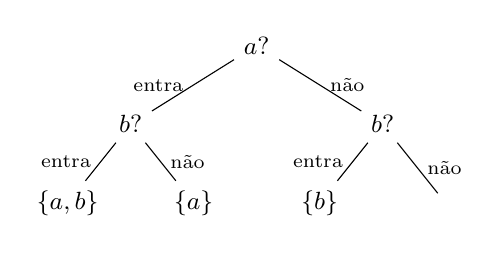
\begin{tikzpicture}[level distance=1.0cm, level 1/.style={sibling distance=3.2cm}, level 2/.style={sibling distance=1.6cm}, every node/.style={font=\small}]
\node {$a$?}
  child {node {$b$?} child {node {$\{a,b\}$} edge from parent node[left]{\scriptsize entra}} child {node {$\{a\}$} edge from parent node[right]{\scriptsize não}} edge from parent node[left]{\scriptsize entra}}
  child {node {$b$?} child {node {$\{b\}$} edge from parent node[left]{\scriptsize entra}} child {node {$\varnothing$} edge from parent node[right]{\scriptsize não}} edge from parent node[right]{\scriptsize não}};
\end{tikzpicture}
\end{center}
  \item Com $n$ elementos, são $n$ decisões de duas opções cada, e cada sequência de decisões dá um subconjunto diferente. Portanto,
\[
n\bigl(\mathcal{P}(A)\bigr)=\underbrace{2\cdot2\cdots2}_{n}=2^{n}.
\]
  \item Os elementos de $\mathcal{P}(A)$ são \emph{conjuntos}. Por isso, $X\in\mathcal{P}(A)$ significa exatamente $X\subset A$: é a ponte entre $\in$ e $\subset$.
\end{enumerate}
\end{construcao}

\begin{definicao}[conjunto das partes]
O \textbf{conjunto das partes} de $A$ é $\mathcal{P}(A)=\{X\mid X\subset A\}$. Se $A$ tem $n$ elementos, $\mathcal{P}(A)$ tem $2^n$ elementos.
\end{definicao}

\begin{paralembrar}\label{lembrar-u2}
\textbf{Dois conjuntos são iguais quando têm os mesmos elementos; ser parte ($\subset$) é \enquote{todo elemento de um está no outro}; ser elemento ($\in$) é \enquote{ser um dos listados}.}
\begin{enumerate}[label=\arabic*.,leftmargin=1.4em,itemsep=1pt]
  \item Para provar $A=B$, prove $A\subset B$ e $B\subset A$.
  \item Para provar $A\subset B$, tome um elemento qualquer de $A$ e mostre que ele está em $B$; para provar $A\not\subset B$, basta uma testemunha.
  \item Para contar subconjuntos, decida elemento a elemento: $2^n$.
\end{enumerate}
\end{paralembrar}

% ------------------------------------------------------------
\OndeEUsado

As ideias desta unidade aparecem em três tipos de enunciado: os que pedem para classificar sentenças com $\in$ e $\subset$, os que pedem uma justificativa ou uma prova, e os que pedem para contar subconjuntos.

\subsubsection{Mapa do problema}

\begin{caso}{1 · \enquote{classifique em V ou F} com $\in$ e $\subset$}{2-U1}
\mapa{sentenças com $\in$, $\notin$, $\subset$, $\not\subset$, muitas vezes com chaves dentro de chaves}
{o que está do lado esquerdo do símbolo: um objeto (pergunta de $\in$) ou um conjunto (pergunta de $\subset$)}
{2-H2 (5): $\in$ procura na lista de elementos; $\subset$ testa cada elemento}
\reconhecer O comando costuma ser seco: \enquote{Diga se é verdadeira (V) ou falsa (F) cada uma das sentenças abaixo}.\src{fme} O sinal é a mistura de símbolos e de chaves: $\{a\}$ pode ser elemento de um conjunto (se estiver listado) e também subconjunto (se $a$ estiver listado). Leia cada sentença em voz alta — \enquote{é um dos elementos?} ou \enquote{todos os elementos estão lá?} — antes de responder. Treino: \exref{ex:u2:chaves}; questões \ref{u2:fme20} e \ref{u2:fme47}.
\end{caso}

\begin{caso}{2 · \enquote{prove}, \enquote{mostre}, \enquote{justifique}}{2-U2}
\mapa{\enquote{mostre que $A\subset B$}, \enquote{prove que $A=B$}, \enquote{classifique e justifique}}
{o \enquote{todo} escondido na definição de $\subset$ e um elemento genérico}
{2-H3: elemento qualquer, ida e volta; testemunha para $\not\subset$}
\reconhecer O verbo pede um argumento, não uma conta. Se a sentença é de inclusão e você acha que é verdadeira, a justificativa precisa valer para \emph{todo} elemento; se acha que é falsa, uma testemunha basta. Treino: \exref{ex:u2:fme18} e \exref{ex:u2:multiplos}; \qref{u2:multiplos4}.
\end{caso}

\begin{caso}{3 · \enquote{quantos subconjuntos\ldots?}}{2-U3}
\mapa{\enquote{quantos subconjuntos}, \enquote{quantos conjuntos $X$ satisfazem $A\subset X\subset B$}, \enquote{de quantas maneiras escolher alguns de\ldots}}
{quais elementos são obrigatórios, quais são proibidos e quais são livres}
{2-H4: cada elemento livre dobra a contagem; com $k$ livres, $2^k$}
\reconhecer O sinal é uma escolha de \enquote{alguns} elementos sem ordem, com ou sem restrições. Em vez de listar, separe os elementos em três grupos — os que precisam entrar, os que não podem entrar e os livres — e conte só as decisões livres. Treino: \exref{ex:u2:partes}; questões \ref{u2:fme35} e \ref{u2:contar}.
\end{caso}

\subsubsection{Tabela de gatilhos}
\begin{gatilhos}
\enquote{V ou F} com chaves aninhadas & 2-H2 (5) & $\in$ procura na lista; $\subset$ testa cada elemento & \mbox{2-U1\,·\,q.\,\ref{u2:fme20}}\\\fino
\enquote{prove}, \enquote{mostre}, \enquote{justifique} & 2-H3 & elemento genérico, ida e volta & \mbox{2-U2\,·\,q.\,\ref{u2:multiplos4}}\\\fino
\enquote{não está contido} & 2-H2 (2) & procurar uma testemunha & \mbox{2-E3\,·\,q.\,\ref{u2:exemplos}}\\\fino
\enquote{quantos subconjuntos} & 2-H4 & contar os elementos livres: $2^k$ & \mbox{2-U3\,·\,q.\,\ref{u2:fme35}}\\
\end{gatilhos}

% ============================================================
% Unidade 2 — Parte B: erros, observações, exemplos, questões, síntese, respostas
% Fonte única: dossies/u2.md · respostas conferidas em verif/u2.py
% ============================================================
\ErrosComuns

\begin{erro}{Trocar $\in$ por $\subset$}{2-E1}
\campo{O erro.} Escrever $\{3\}\in\{1,3,5\}$ ou $3\subset\{1,3,5\}$.
\campo{Por que parece plausível.} \enquote{O 3 está lá dentro}, e em português \enquote{está em} serve para as duas coisas.
\campo{Onde quebra.} Os elementos de $\{1,3,5\}$ são 1, 3 e 5; o conjunto $\{3\}$ não é nenhum deles, logo $\{3\}\notin\{1,3,5\}$. E o número 3 não é um conjunto, então \enquote{$3\subset\ldots$} não faz sentido. O correto é $3\in\{1,3,5\}$ e $\{3\}\subset\{1,3,5\}$.
\campo{Como detectar.} Olhe o lado esquerdo do símbolo. Se é um objeto, a pergunta é de $\in$: procure-o na lista. Se é um conjunto, a pergunta costuma ser de $\subset$: procure cada um dos seus elementos — ou de $\in$, se esse conjunto aparecer listado como elemento.
\campo{Como corrigir.} Leia $\in$ como \enquote{é um dos elementos de} e $\subset$ como \enquote{todos os elementos de\ldots{} estão em\ldots} (construção 2-H2).
\campo{Onde aparece.} \exref{ex:u2:chaves}; questões \ref{u2:fme20} e \ref{u2:fme47}.
\end{erro}

\begin{erro}{Inverter o papel do vazio}{2-E2}
\campo{O erro.} Achar que $\varnothing\in A$ para todo conjunto $A$, ou que $\varnothing\subset A$ só quando $A$ \enquote{tem o vazio}.
\campo{Por que parece plausível.} \enquote{O vazio está em todo lugar}.
\campo{Onde quebra.} Em $A=\{7,8\}$, os elementos são 7 e 8: $\varnothing\notin A$. Mas $\varnothing\subset A$, como em qualquer conjunto (construção 2-H2). Já em $\{\varnothing,7\}$ o vazio está listado, e aí $\varnothing\in\{\varnothing,7\}$.
\campo{Como detectar.} Para $\in$, procure \enquote{$\varnothing$} escrito entre as chaves. Para $\subset$, a resposta é sempre \enquote{sim}.
\campo{Como corrigir.} Separe as perguntas: \enquote{o vazio está na lista?} (pertinência) e \enquote{algum elemento do vazio fica de fora?} (inclusão — nunca, porque o vazio não tem elementos).
\campo{Onde aparece.} \exref{ex:u2:chaves}; questões \ref{u2:fme20} e \ref{u2:fme47}.
\end{erro}

\begin{erro}{Negar \enquote{$A\subset B$} como \enquote{$B\subset A$}}{2-E3}
\campo{O erro.} De \enquote{$A$ não está contido em $B$} concluir que \enquote{então $B$ está contido em $A$}.
\campo{Por que parece plausível.} Parece que só há duas possibilidades, como em \enquote{maior} e \enquote{menor}.
\campo{Onde quebra.} Com $A=\{1,2\}$ e $B=\{2,3\}$: $A\not\subset B$ (1 é testemunha) e também $B\not\subset A$ (3 é testemunha).
\campo{Como detectar.} Procure uma testemunha em cada sentido; podem existir as duas.
\campo{Como corrigir.} $A\not\subset B$ é a negação de \enquote{para todo $x$, se $x\in A$, então $x\in B$}: existe $x\in A$ com $x\notin B$ (negação do condicional, Cap.~I). Isso não diz nada sobre $B\subset A$.
\campo{Onde aparece.} \exref{ex:u2:fme18}; \qref{u2:exemplos}.
\end{erro}

\begin{erro}{Provar com exemplos, ou com um lado só}{2-E4}
\campo{O erro.} Dizer \enquote{testei 6, 12 e 18 e deu certo} como prova de que dois conjuntos são iguais; ou provar só $A\subset B$ e concluir $A=B$.
\campo{Por que parece plausível.} Os exemplos convencem, e \enquote{estar contido} parece quase \enquote{ser igual}.
\campo{Onde quebra.} A igualdade $x^2=x$ vale para 0 e para 1 e falha para 2: exemplos não garantem o \enquote{todo}. E $\mathbb{N}\subset\mathbb{Z}$, mas $\mathbb{N}\neq\mathbb{Z}$.
\campo{Como detectar.} Pergunte: o argumento usa um elemento \emph{qualquer}, ou números escolhidos? Os dois sentidos foram provados?
\campo{Como corrigir.} Use o elemento genérico e a dupla inclusão (construção 2-H3).
\campo{Onde aparece.} \exref{ex:u2:multiplos}; \qref{u2:multiplos4}.
\end{erro}

\begin{erro}{Contar subconjuntos esquecendo o vazio ou o todo}{2-E5}
\campo{O erro.} Dizer que $\{a,b,c\}$ tem 6 subconjuntos: os três de um elemento e os três de dois elementos.
\campo{Por que parece plausível.} \enquote{Parte} sugere um pedaço menor e não vazio.
\campo{Onde quebra.} Pela definição, $\varnothing\subset\{a,b,c\}$ e $\{a,b,c\}\subset\{a,b,c\}$. São $8=2^3$ subconjuntos.
\campo{Como detectar.} Compare o total com $2^n$.
\campo{Como corrigir.} Monte a lista pela árvore \enquote{entra / não entra} (construção 2-H4): ela inclui as duas escolhas extremas, \enquote{ninguém entra} e \enquote{todos entram}.
\campo{Onde aparece.} \exref{ex:u2:partes}; questões \ref{u2:fme22} e \ref{u2:contar}.
\end{erro}

% ------------------------------------------------------------
\Observacoes

\begin{obs}{2-O1}
\textbf{Outra notação para \enquote{contido}.} Neste material, $A\subset B$ admite $A=B$. Muitos livros escrevem $A\subseteq B$ para isso e reservam $A\subset B$, ou $A\subsetneq B$, para o caso em que $A$ é um \textbf{subconjunto próprio} de $B$ (contido e diferente).\src{gardnerNotes} Ao ler outro texto, confira qual convenção ele usa.
\end{obs}

\begin{obs}{2-O2}
\textbf{Uma parte tão grande quanto o todo.} Em 1638, no livro \emph{Duas novas ciências}, Galileu Galilei pôs seus personagens para comparar os números naturais $1,2,3,\ldots$ com os quadrados $1,4,9,\ldots$. Os quadrados são só uma parte dos números; mas cada número é raiz de exatamente um quadrado, e cada quadrado tem exatamente uma raiz, de modo que os dois se emparelham um a um.\src{galileu1638}\src{blaszczyk2021} A conclusão de Galileu foi que, no infinito, \enquote{maior}, \enquote{menor} e \enquote{igual} não funcionam como nas coleções finitas. Em conjuntos finitos, um subconjunto próprio sempre tem menos elementos; em conjuntos infinitos, não necessariamente.
\end{obs}

\begin{obs}{2-O3}
\textbf{Elementos que não são conjuntos.} Neste material, um elemento pode ser um objeto que não é conjunto — uma letra, um número, uma pessoa. Esses objetos se chamam \emph{urelementos}. A teoria de Zermelo de 1908 os admitia; as teorias usadas hoje como fundamento da matemática dispensam esses objetos e trabalham só com conjuntos, de modo que lá todo elemento é, ele próprio, um conjunto.\src{nlabZFA}\src{zermelo1908}
\end{obs}

% ------------------------------------------------------------
\Exemplos

\begin{exemplo}{}{1}{FME, exercício 17}{2-H1, 2-H2, 2-U1}
\label{ex:u2:fme17}
Dados $A=\{1,2,3,4\}$ e $B=\{2,4\}$:
\begin{enumerate}[label=\alph*)]
  \item escreva com os símbolos da teoria dos conjuntos as sentenças: 1ª) 3 é elemento de $A$; 2ª) 1 não está em $B$; 3ª) $B$ é parte de $A$; 4ª) $B$ é igual a $A$; 5ª) 4 pertence a $B$;
  \item classifique as sentenças anteriores em falsas ou verdadeiras.
\end{enumerate}
\plano Traduzir cada expressão (\enquote{é elemento de}, \enquote{está em}, \enquote{pertence a} $\to\in$; \enquote{é parte de} $\to\subset$) e conferir na lista.
\resolucao 1ª) $3\in A$ (V); 2ª) $1\notin B$ (V); 3ª) $B\subset A$ (V: 2 e 4 estão em $A$); 4ª) $B=A$ (F: 1 é testemunha); 5ª) $4\in B$ (V).
\comentario Na 3ª, a verificação passa por \emph{todos} os elementos de $B$; na 4ª, um único elemento de $A$ fora de $B$ basta para a desigualdade.
\end{exemplo}

\begin{exemplo}{}{1}{FME, exercício 18}{2-H2, 2-U2, 2-E3}
\label{ex:u2:fme18}
Sendo $A=\{1,2\}$, $B=\{2,3\}$, $C=\{1,3,4\}$ e $D=\{1,2,3,4\}$, classifique em V ou F cada sentença abaixo e justifique.
\begin{multicols}{3}
\begin{enumerate}[label=\alph*)]
  \item $A\subset D$
  \item $A\subset B$
  \item $B\subset C$
  \item $D\supset B$
  \item $C=D$
  \item $A\not\subset C$
\end{enumerate}
\end{multicols}
\plano Para uma inclusão verdadeira, conferir todos os elementos; para uma falsa, achar uma testemunha.
\resolucao a) V, pois $1\in D$ e $2\in D$. b) F, pois $1\in A$ e $1\notin B$. c) F, pois $2\in B$ e $2\notin C$. d) V, pois $2\in D$ e $3\in D$. e) F, pois $2\in D$ e $2\notin C$. f) V, pois $2\in A$ e $2\notin C$.
\comentario Em (b), também vale $B\not\subset A$ (3 é testemunha): uma inclusão falsa não garante a inclusão contrária (erro 2-E3).
\end{exemplo}

\begin{exemplo}{}{2}{autoral}{2-H2, 2-U1, 2-E1, 2-E2}
\label{ex:u2:chaves}
Seja $E=\{1,\{1\},\{2,3\}\}$. Classifique em V ou F:
\begin{multicols}{4}
\begin{enumerate}[label=\alph*)]
  \item $1\in E$
  \item $\{1\}\in E$
  \item $\{1\}\subset E$
  \item $\{2\}\subset E$
  \item $\{2,3\}\in E$
  \item $\{2,3\}\subset E$
  \item $\varnothing\subset E$
  \item $\varnothing\in E$
\end{enumerate}
\end{multicols}
\plano Listar primeiro os elementos de $E$: são três, o número 1, o conjunto $\{1\}$ e o conjunto $\{2,3\}$. Depois, para cada sentença, decidir se a pergunta é \enquote{está na lista?} ($\in$) ou \enquote{todos os elementos estão na lista?} ($\subset$).
\resolucao a) V. b) V: $\{1\}$ é o segundo elemento listado. c) V: o único elemento de $\{1\}$, o 1, está em $E$. d) F: $2\notin E$ (2 está \emph{dentro} de um elemento de $E$, mas não é elemento de $E$). e) V. f) F: $2\notin E$. g) V: o vazio está contido em qualquer conjunto. h) F: o vazio não está listado.
\comentario Em (b) e (c), $\{1\}$ é ao mesmo tempo elemento e subconjunto de $E$ — isso só acontece porque $E$ lista tanto o 1 quanto o $\{1\}$. Em (e) e (f), $\{2,3\}$ é elemento, mas não subconjunto.
\end{exemplo}

\begin{exemplo}{}{2}{autoral}{2-H3, 2-U2, 2-E4}
\label{ex:u2:multiplos}
Prove que $\{x\in\mathbb{Z}\mid x\text{ é múltiplo de 2 e de 3}\}=\{x\in\mathbb{Z}\mid x\text{ é múltiplo de 6}\}$.
\plano Dupla inclusão, com um elemento genérico em cada sentido.
\resolucao Chame os conjuntos de $A$ e $B$. \emph{$B\subset A$:} se $x\in B$, então $x=6k$ para algum inteiro $k$; logo $x=2\cdot(3k)$ e $x=3\cdot(2k)$, e $x$ é múltiplo de 2 e de 3: $x\in A$. \emph{$A\subset B$:} se $x\in A$, então $x=2a$ para algum inteiro $a$, e 3 divide $2a$. Como 3 não divide 2, e 3 é primo, 3 divide $a$: $a=3b$, e $x=6b$. Logo $x\in B$. Pelas duas inclusões, $A=B$.
\comentario Testar $6$, $12$ e $18$ não provaria nada (erro 2-E4): a prova usou um $x$ qualquer, sem escolher qual.
\end{exemplo}

\begin{exemplo}{}{2}{autoral}{2-H4, 2-U3, 2-E5}
\label{ex:u2:partes}
\begin{enumerate}[label=\alph*)]
  \item Liste os elementos de $\mathcal{P}(\{a,b,c\})$.
  \item Quantos subconjuntos de $\{1,2,3,4,5\}$ contêm o número 1?
\end{enumerate}
\plano Em (a), seguir a árvore \enquote{entra / não entra}. Em (b), separar os elementos obrigatórios dos livres.
\resolucao a) $\varnothing$, $\{a\}$, $\{b\}$, $\{c\}$, $\{a,b\}$, $\{a,c\}$, $\{b,c\}$, $\{a,b,c\}$: são $8=2^3$. b) O 1 tem de entrar; 2, 3, 4 e 5 são livres. São $2^4=16$ subconjuntos.
\comentario Em (a), o vazio e o próprio conjunto entram na conta (erro 2-E5). Em (b), a decisão sobre o 1 já está tomada; só as decisões livres multiplicam.
\end{exemplo}

\begin{exemplo}{}{3}{autoral}{2-H2, 2-H3}
\label{ex:u2:vazio}
Prove que existe um único conjunto vazio: se $\varnothing_1$ e $\varnothing_2$ são conjuntos sem elementos, então $\varnothing_1=\varnothing_2$.
\plano Usar a construção 2-H3: provar as duas inclusões. Para cada uma, usar o fato de que o vazio está contido em qualquer conjunto.
\resolucao Como $\varnothing_1$ não tem elementos, a sentença \enquote{se $x\in\varnothing_1$, então $x\in\varnothing_2$} é verdadeira para todo $x$ (hipótese sempre falsa); logo $\varnothing_1\subset\varnothing_2$. Trocando os papéis, $\varnothing_2\subset\varnothing_1$. Pela dupla inclusão, $\varnothing_1=\varnothing_2$.
\comentario A Unidade~1 \emph{afirmou} que todos os conjuntos sem elementos são o mesmo; aqui está a prova. A novidade é usar a vacuidade nos dois sentidos para concluir uma igualdade.
\end{exemplo}

% ------------------------------------------------------------
\Questoes

\begin{questao}{1}{autoral}{2-H2, 2-U1}\label{u2:completar}
Seja $A=\{2,4,6\}$. Complete com $\in$, $\notin$, $\subset$, $\not\subset$ ou $=$:
\begin{multicols}{3}
\begin{enumerate}[label=\alph*)]
  \item $2\ \_\ A$
  \item $\{2\}\ \_\ A$
  \item $\{2,5\}\ \_\ A$
  \item $\{6,4,2\}\ \_\ A$
  \item $5\ \_\ A$
\end{enumerate}
\end{multicols}
\resp{a) $\in$;\ b) $\subset$;\ c) $\not\subset$;\ d) $=$ (também vale $\subset$);\ e) $\notin$.}
\end{questao}

\begin{questao}{1}{FME, exercício 19}{2-H1}\label{u2:fme19}
Quais das igualdades abaixo são verdadeiras?
\begin{enumerate}[label=\alph*)]
  \item $\{a,a,a,b,b\}=\{a,b\}$
  \item $\{x\mid x^2=4\}=\{x\mid x\neq0\text{ e }x^3-4x=0\}$
  \item $\{x\mid 2x+7=11\}=\{2\}$
  \item $\{x\mid x<0\text{ e }x\ge0\}=\varnothing$
\end{enumerate}
\resp{Todas são verdadeiras.}
\end{questao}

\begin{questao}{1}{FME, exercício 22}{2-H4, 2-E5}\label{u2:fme22}
Construa o conjunto das partes do conjunto $A=\{a,b,c,d\}$.
\resp{16 elementos: $\varnothing$, $\{a\}$, $\{b\}$, $\{c\}$, $\{d\}$, $\{a,b\}$, $\{a,c\}$, $\{a,d\}$, $\{b,c\}$, $\{b,d\}$, $\{c,d\}$, $\{a,b,c\}$, $\{a,b,d\}$, $\{a,c,d\}$, $\{b,c,d\}$, $\{a,b,c,d\}$.}
\end{questao}

\begin{questao}{1}{FME, exercício 21}{2-H2}\label{u2:fme21}
Faça um diagrama de Venn que simbolize a situação seguinte: $A$, $B$, $C$ e $D$ são conjuntos não vazios, $D\subset C\subset B\subset A$.
\resp{Quatro regiões encaixadas: a de $D$ dentro da de $C$, a de $C$ dentro da de $B$ e a de $B$ dentro da de $A$.}
\end{questao}

\begin{questao}{2}{FME, exercício 20}{2-H2, 2-U1, 2-E1, 2-E2}\label{u2:fme20}
Diga se é verdadeira (V) ou falsa (F) cada uma das sentenças abaixo.
\begin{multicols}{2}
\begin{enumerate}[label=\alph*)]
  \item $0\in\{0,1,2,3,4\}$
  \item $\{a\}\in\{a,b\}$
  \item $\varnothing\in\{0\}$
  \item $0\in\varnothing$
  \item $\{a\}\subset\varnothing$
  \item $a\in\{a,\{a\}\}$
  \item $\{a\}\subset\{a,\{a\}\}$
  \item $\varnothing\subset\{\varnothing,\{a\}\}$
  \item $\varnothing\in\{\varnothing,\{a\}\}$
  \item $\{a,b\}\in\{a,b,c,d\}$
\end{enumerate}
\end{multicols}
\resp{a) V;\ b) F;\ c) F;\ d) F;\ e) F;\ f) V;\ g) V;\ h) V;\ i) V;\ j) F.}
\end{questao}

\begin{questao}{2}{adaptado do FME, exercício 47}{2-H2, 2-U1, 2-E1, 2-E2}\label{u2:fme47}
Seja $E=\{a,\{a\}\}$, em que $a$ é um objeto que não é conjunto. Diga quais das proposições abaixo são verdadeiras.
\begin{multicols}{3}
\begin{enumerate}[label=\alph*)]
  \item $a\in E$
  \item $\{a\}\in E$
  \item $a\subset E$
  \item $\{a\}\subset E$
  \item $\varnothing\in E$
  \item $\varnothing\subset E$
\end{enumerate}
\end{multicols}
\resp{a, b, d, f.}
\end{questao}

\begin{questao}{2}{autoral}{2-H2, 2-E3}\label{u2:exemplos}
Dê exemplos de conjuntos $A$ e $B$ tais que:
\begin{enumerate}[label=\alph*)]
  \item $A\not\subset B$ e $B\subset A$;
  \item $A\not\subset B$ e $B\not\subset A$;
  \item $A\subset B$ e $B\subset A$.
\end{enumerate}
O que a condição do item (c) obriga?
\resp{Por exemplo: a) $A=\{1,2\}$, $B=\{1\}$;\ b) $A=\{1\}$, $B=\{2\}$;\ c) $A=B=\{1\}$. A condição (c) obriga $A=B$.}
\end{questao}

\begin{questao}{2}{autoral}{2-H2, 2-H3, 2-U2, 2-E4}\label{u2:multiplos4}
Prove que $\{x\in\mathbb{Z}\mid x\text{ é múltiplo de 4}\}\subset\{x\in\mathbb{Z}\mid x\text{ é par}\}$ e mostre que a inclusão contrária é falsa.
\resp{Demonstração. A prova deve mostrar que um múltiplo qualquer de 4, $x=4k$, se escreve como $x=2\cdot(2k)$, logo é par; e dar uma testemunha da inclusão contrária, como 2, que é par e não é múltiplo de 4.}
\end{questao}

\begin{questao}{2}{FME, exercício 35}{2-H4, 2-U3}\label{u2:fme35}
Determine o número de conjuntos $X$ que satisfazem a relação $\{1,2\}\subset X\subset\{1,2,3,4\}$.
\resp{4.}
\end{questao}

\begin{questao}{2}{autoral}{2-H4, 2-U3, 2-E5}\label{u2:contar}
\begin{enumerate}[label=\alph*)]
  \item Um conjunto $A$ é tal que $\mathcal{P}(A)$ tem 64 elementos. Quantos elementos tem $A$?
  \item Quantos subconjuntos de um conjunto de 5 elementos não são nem o vazio nem o próprio conjunto?
\end{enumerate}
\resp{a) 6;\ b) $2^5-2=30$.}
\end{questao}

\begin{questao}[integradora]{2}{autoral}{2-H4, 2-U3}\label{u2:divisores}
Quantos subconjuntos do conjunto dos divisores naturais de 12 contêm o 1 e o 12?
\resp{16 (os divisores são 1, 2, 3, 4, 6 e 12; o 1 e o 12 são obrigatórios e os outros quatro, livres: $2^4$).}
\end{questao}

\begin{questao}{3}{autoral}{2-H4, 2-E1}\label{u2:vazios3}
Escreva $\mathcal{P}(\varnothing)$, $\mathcal{P}(\mathcal{P}(\varnothing))$ e $\mathcal{P}(\mathcal{P}(\mathcal{P}(\varnothing)))$ e diga quantos elementos tem cada um.
\resp{$\mathcal{P}(\varnothing)=\{\varnothing\}$ (1 elemento);\ $\mathcal{P}(\mathcal{P}(\varnothing))=\{\varnothing,\{\varnothing\}\}$ (2);\ $\mathcal{P}(\mathcal{P}(\mathcal{P}(\varnothing)))=\{\varnothing,\{\varnothing\},\{\{\varnothing\}\},\{\varnothing,\{\varnothing\}\}\}$ (4).}
\end{questao}

\begin{questao}{3}{ITA via FME, ano não informado; adaptado: a alternativa e repetia a a}{2-H2, 2-H4}\label{u2:cadeias}
Seja $U$ um conjunto não vazio com $n$ elementos, $n\ge1$. Seja $S$ um subconjunto de $\mathcal{P}(U)$ com a seguinte propriedade: se $A,B\in S$, então $A\subset B$ ou $B\subset A$. Então, o número máximo de elementos que $S$ pode ter é:
\begin{enumerate}[label=\alph*)]
  \item $2^{n-1}$
  \item $\frac{n}{2}$, se $n$ for par, e $\frac{n+1}{2}$, se $n$ for ímpar
  \item $n+1$
  \item $2^{n-1}+1$
  \item $2^{n}-1$
\end{enumerate}
\resp{c.}
\end{questao}

\begin{questao}{3}{autoral}{2-H4, 2-U3}\label{u2:paridade}
Quantos subconjuntos de $\{1,2,\ldots,n\}$, com $n\ge1$, têm um número par de elementos? Justifique.
\resp{$2^{n-1}$. Demonstração. A prova deve mostrar que, pondo ou tirando o 1, os subconjuntos se agrupam em pares formados por um de tamanho par e um de tamanho ímpar; logo exatamente metade dos $2^n$ tem tamanho par.}
\end{questao}

\begin{sintese}
\textbf{Ao fim desta unidade, você deveria saber:}
\begin{itemize}[leftmargin=1.4em,itemsep=1pt]
  \item decidir se dois conjuntos são iguais e justificar com os elementos;
  \item distinguir $\in$ de $\subset$, inclusive com chaves dentro de chaves e com o vazio;
  \item provar uma inclusão com um elemento genérico e uma igualdade com duas inclusões;
  \item negar uma inclusão com uma testemunha;
  \item listar e contar os subconjuntos de um conjunto finito.
\end{itemize}
\smallskip\noindent\textbf{Responda com suas palavras, sem consultar.} Depois, confira com a caixa \emph{Para lembrar} (p.~\pageref{lembrar-u2}) e com a seção indicada.
\begin{enumerate}[label=\arabic*.,leftmargin=1.4em]
  \perguntasintese{Por que $\{a,b\}$ e $\{b,a,a\}$ são o mesmo conjunto? \ondever{construção 2-H1}}
  \perguntasintese{Qual é a diferença entre $x\in A$ e $X\subset A$? Por que $X\in\mathcal{P}(A)$ significa o mesmo que $X\subset A$? \ondever{De onde vem?}}
  \perguntasintese{Num enunciado, que sinais indicam que você precisa de uma prova com elemento genérico? E que sinais indicam uma contagem de subconjuntos? \ondever{Onde é usado?}}
  \perguntasintese{Qual destes erros você comete com mais facilidade — trocar $\in$ por $\subset$, ou esquecer o vazio? Como você o detecta? \ondever{Erros comuns}}
\end{enumerate}
\end{sintese}

% ------------------------------------------------------------
\Respostas
{\small\resposta{S}{Síntese de domínio: confira com a caixa \emph{Para lembrar} (p.~\pageref{lembrar-u2}) e com a seção indicada em cada pergunta.}}


% ============================================================
% Unidade 3 — Reunião e interseção   (didática v4 · kit/didatica.md §2)
% Parte A, o "artigo": Prefácio, De onde vem?, Onde é usado?
% IDs: 3-H1..H4 · 3-U1..U4 · 3-E1..E4 · 3-O1, 3-O2 (matriz.yaml) · fonte única: dossies/u3.md
% ============================================================
\clearpage
\section{Reunião e interseção}

% ------------------------------------------------------------
\Prefacio
\begin{prefacio}
\gancho{\enquote{Ou} amplia, \enquote{e} restringe}

Um site de vagas permite filtrar candidatos por dois critérios. Com o filtro \enquote{fala inglês \textbf{ou} usa planilhas}, a lista cresce: entra quem tem pelo menos uma das duas habilidades. Com \enquote{fala inglês \textbf{e} usa planilhas}, a lista encolhe: só fica quem tem as duas. Quem tem as duas aparece nas duas buscas — e, na primeira, aparece uma vez só, não duas.

No Capítulo I, \enquote{ou} e \enquote{e} ligavam proposições. Aqui, as mesmas palavras ligam conjuntos e produzem conjuntos novos. \textbf{Como o \enquote{ou} e o \enquote{e} da lógica viram operações entre conjuntos?}

\textbf{Ao final, você será capaz de:} calcular reuniões e interseções; transformar o \enquote{ou} e o \enquote{e} de uma condição em reunião e interseção de conjuntos-solução; usar as propriedades das operações, inclusive as distributivas; descobrir um conjunto desconhecido a partir de condições, elemento a elemento; decidir se uma propriedade vale para quaisquer conjuntos.

\textbf{Pré-requisitos:} Unidades 1 e 2; do Capítulo I, os conectivos \enquote{ou} e \enquote{e}, as tabelas-verdade e as propriedades desses conectivos. O essencial está na caixa abaixo.
\end{prefacio}

\begin{minimo}
\begin{itemize}[leftmargin=1.4em,itemsep=1pt]
  \item \textbf{\enquote{Ou} inclusivo.} \enquote{$p$ ou $q$} ($p\vee q$) é verdadeira quando pelo menos uma das duas é verdadeira — inclusive quando as duas são (Cap.~I).
  \item \textbf{\enquote{E}.} \enquote{$p$ e $q$} ($p\wedge q$) é verdadeira só quando as duas são verdadeiras (Cap.~I).
  \item \textbf{Inclusão e igualdade.} $A\subset B$: todo elemento de $A$ está em $B$; $A=B$: $A\subset B$ e $B\subset A$ (Unidade~2).
\end{itemize}
\end{minimo}

% ------------------------------------------------------------
\DeOndeVem

\subsubsection{Por que alguém precisou disso}
Conjuntos raramente aparecem sozinhos. Juntamos duas listas (quem fala inglês ou espanhol), cruzamos dois critérios (quem fala inglês e espanhol), exigimos duas condições ao mesmo tempo (um sistema de equações). Precisamos de operações que, a partir de dois conjuntos, produzam um terceiro — e de regras para calcular com elas sem precisar voltar, toda vez, aos elementos.

\subsubsection{A reunião e a interseção}
\begin{construcao}[reunião e interseção]{3-H1}
\begin{enumerate}[label=(\arabic*)]
  \item A \textbf{reunião} de $A$ e $B$ é o conjunto dos elementos que pertencem a $A$ \emph{ou} a $B$:\src{fme}
\[
A\cup B=\{x\mid x\in A\ \text{ou}\ x\in B\}.
\]
Lê-se \enquote{$A$ reunião $B$}. São os elementos que pertencem a \emph{pelo menos um} dos dois conjuntos.
  \item A \textbf{interseção} de $A$ e $B$ é o conjunto dos elementos que pertencem a $A$ \emph{e} a $B$:\src{fme}
\[
A\cap B=\{x\mid x\in A\ \text{e}\ x\in B\}.
\]
Lê-se \enquote{$A$ inter $B$}. São os elementos que pertencem aos dois ao mesmo tempo.
  \item O \enquote{ou} da reunião é o da lógica, \emph{inclusivo}: quem está nos dois conjuntos está na reunião — e entra uma vez só, porque um conjunto não registra repetições (Unidade~2).
  \item Exemplos: $\{a,b\}\cup\{c,d\}=\{a,b,c,d\}$; $\{a,b,c\}\cup\{c,d,e\}=\{a,b,c,d,e\}$; $\{a,b,c\}\cap\{b,c,d,e\}=\{b,c\}$; $\{a,b\}\cap\{c,d\}=\varnothing$; $\{a,b\}\cup\varnothing=\{a,b\}$; $\{a,b\}\cap\varnothing=\varnothing$.\src{fme}
\end{enumerate}
\end{construcao}

\begin{definicao}[reunião, interseção, conjuntos disjuntos]
$A\cup B=\{x\mid x\in A\text{ ou }x\in B\}$ e $A\cap B=\{x\mid x\in A\text{ e }x\in B\}$. Quando $A\cap B=\varnothing$, isto é, quando $A$ e $B$ não têm elemento comum, $A$ e $B$ são chamados \textbf{disjuntos}.\src{fme}
\end{definicao}

\subsubsection{Boole: o produto, a soma e a reunião}
A ideia de calcular com classes como se calcula com números é do matemático George Boole, que publicou dois livros sobre o assunto, em 1847 e em 1854. Boole representava cada classe por uma letra e escrevia $xy$ para a classe dos objetos que são, ao mesmo tempo, $X$ e $Y$ — a interseção, em linguagem de hoje. Para \enquote{juntar} classes, usava $x+y$, mas só quando as duas classes não tinham membros em comum; sem essa condição, ele considerava a expressão sem interpretação.\src{sepAlgLog}\src{burrisTalk}\src{boole1854} Lido hoje, o \enquote{$+$} de Boole é a reunião de conjuntos disjuntos. Em 1864, o lógico William Stanley Jevons trocou essa operação restrita pela reunião sem restrição, que é o $\cup$ usado até hoje.\src{sepAlgLog}

Boole também já escrevia leis como $x(y+z)=xy+xz$ e $xx=x$.\src{sepAlgLog}\src{boole1854} É por isso que as propriedades de $\cup$ e $\cap$ lembram as da aritmética — e é também por isso que é preciso cuidado: elas \emph{não} são as da aritmética.

\subsubsection{As propriedades vêm da lógica}
\begin{construcao}[propriedades da reunião e da interseção]{3-H2}
\begin{enumerate}[label=(\arabic*)]
  \item Escreva $A=\{x\mid p(x)\}$ e $B=\{x\mid q(x)\}$. Pela construção 3-H1,
\[
A\cup B=\{x\mid p(x)\vee q(x)\}\qquad\text{e}\qquad A\cap B=\{x\mid p(x)\wedge q(x)\}.
\]
  \item Toda equivalência entre proposições vira uma igualdade entre conjuntos. Como \enquote{$p$ ou $p$} equivale a $p$, temos $A\cup A=A$; como \enquote{$p$ ou $q$} equivale a \enquote{$q$ ou $p$}, temos $A\cup B=B\cup A$. Do mesmo modo, para conjuntos quaisquer $A$, $B$ e $C$:\src{fme}
\begin{center}
\begin{tabular}{@{}lll@{}}
 & reunião & interseção\\\midrule
idempotente & $A\cup A=A$ & $A\cap A=A$\\
comutativa & $A\cup B=B\cup A$ & $A\cap B=B\cap A$\\
associativa & $(A\cup B)\cup C=A\cup(B\cup C)$ & $(A\cap B)\cap C=A\cap(B\cap C)$\\
elemento neutro & $A\cup\varnothing=A$ & $A\cap U=A$\\
\end{tabular}
\end{center}
  \item Os elementos neutros também vêm da lógica: $\varnothing$ é descrito por uma propriedade sempre falsa, e \enquote{$p$ ou (falsa)} equivale a $p$; o universo $U$ é descrito por uma propriedade sempre verdadeira, e \enquote{$p$ e (verdadeira)} equivale a $p$.
  \item As propriedades lembram as da soma e da multiplicação, mas não são as mesmas: $A\cup A=A$, enquanto $2+2\neq2$.
\end{enumerate}
\end{construcao}

\begin{construcao}[absorção e distributivas]{3-H3}
\begin{enumerate}[label=(\arabic*)]
  \item \textbf{Absorção:} $A\cup(A\cap B)=A$ e $A\cap(A\cup B)=A$.\src{fme} Os elementos de $A\cap B$ já estão em $A$; juntá-los a $A$ não acrescenta nada.
  \item \textbf{Distributivas:}\src{fme}
\[
A\cup(B\cap C)=(A\cup B)\cap(A\cup C)\qquad\text{e}\qquad A\cap(B\cup C)=(A\cap B)\cup(A\cap C).
\]
Elas vêm das distributivas do \enquote{ou} sobre o \enquote{e} e do \enquote{e} sobre o \enquote{ou}, vistas no Capítulo I.
  \item Repare que \emph{as duas} operações distribuem uma sobre a outra. Na aritmética, só a multiplicação distribui sobre a soma: em geral, $a+(b\cdot c)\neq(a+b)\cdot(a+c)$.
\end{enumerate}
\end{construcao}

\subsubsection{Disjuntos e o diagrama de duas regiões}
\begin{construcao}[conjuntos disjuntos e regiões]{3-H4}
\begin{enumerate}[label=(\arabic*)]
  \item Dois conjuntos dividem o universo em quatro regiões: os elementos só de $A$, os dos dois, os só de $B$ e os de nenhum.
\begin{center}
\begin{tikzpicture}[scale=0.9]
\draw[thick] (-3.6,-1.9) rectangle (3.6,1.9); \node at (3.3,1.6) {$U$};
\draw[acento,thick] (-0.85,0) circle (1.45); \draw[acento,thick] (0.85,0) circle (1.45);
\node[font=\scriptsize] at (-1.45,0) {só $A$}; \node[font=\scriptsize] at (0,0) {$A$ e $B$}; \node[font=\scriptsize] at (1.45,0) {só $B$};
\node[font=\scriptsize,anchor=south west] at (-3.55,-1.85) {nenhum};
\node at (-1.95,1.3) {$A$}; \node at (1.95,1.3) {$B$};
\end{tikzpicture}
\end{center}
$A\cup B$ ocupa três regiões (só $A$, $A$ e $B$, só $B$); $A\cap B$, uma.
  \item $A$ e $B$ são \textbf{disjuntos} quando a região \enquote{$A$ e $B$} está vazia: $A\cap B=\varnothing$.\src{fme} Disjuntos não quer dizer vazios: $\{1,2\}$ e $\{7,8\}$ são disjuntos, e nenhum dos dois é vazio.
  \item Quando $A$ e $B$ são disjuntos, contar os elementos de $A\cup B$ é somar — é a situação do \enquote{$+$} de Boole. Quando não são, somar conta duas vezes quem está na região do meio. A Unidade~5 resolve essa contagem.
\end{enumerate}
\end{construcao}

\begin{paralembrar}\label{lembrar-u3}
\textbf{Reunião é \enquote{ou} (pelo menos um); interseção é \enquote{e} (os dois). As propriedades das operações são as propriedades do \enquote{ou} e do \enquote{e}.}
\begin{enumerate}[label=\arabic*.,leftmargin=1.4em,itemsep=1pt]
  \item Para calcular, percorra os elementos e pergunte: está em $A$? está em $B$?
  \item Para provar uma igualdade entre expressões, traduza para a lógica ou compare as regiões do diagrama.
  \item Para achar um conjunto desconhecido, decida elemento a elemento.
\end{enumerate}
\end{paralembrar}

% ------------------------------------------------------------
\OndeEUsado

A reunião e a interseção aparecem sempre que duas condições são combinadas — em buscas, em sistemas, em problemas que pedem um conjunto desconhecido e em sentenças sobre conjuntos quaisquer. São quatro situações.

\subsubsection{Mapa do problema}

\begin{caso}{1 · filtros e listas com \enquote{ou} e \enquote{e}}{3-U1}
\mapa{duas listas, dois critérios ou dois filtros ligados por \enquote{ou} ou por \enquote{e}}
{quem satisfaz \emph{pelo menos um} critério (reunião) ou \emph{os dois} (interseção)}
{3-H1: percorrer os elementos e testar cada critério}
\reconhecer Linguagens de programação trazem as duas operações prontas. No tutorial oficial do Python, com \texttt{a = set('abracadabra')} e \texttt{b = set('alacazam')}, a expressão \texttt{a | b} dá as letras que estão em \texttt{a}, em \texttt{b} ou em ambos, e \texttt{a \& b} dá as letras que estão nos dois.\src{pyTut} Leia \texttt{|} como \enquote{ou} e \texttt{\&} como \enquote{e}: o resultado é $\{a,b,r,c,d,l,z,m\}$ e $\{a,c\}$. Treino: \exref{ex:u3:operar}; questões \ref{u3:fme23} e \ref{u3:fme28}.
\end{caso}

\begin{caso}{2 · condições compostas}{3-U2}
\mapa{uma condição com \enquote{ou} (\enquote{$x=\ldots$ ou $x=\ldots$}, um produto igual a zero) ou com \enquote{e} (um sistema, duas desigualdades)}
{o conjunto-solução de cada parte separadamente}
{3-H1: \enquote{ou} entre condições $\to$ reunião dos conjuntos-solução; \enquote{e} $\to$ interseção}
\reconhecer O sinal é a palavra que liga as condições. Resolva cada parte sozinha, no mesmo universo, e só depois junte: com \enquote{ou}, fica tudo o que resolve pelo menos uma parte; com \enquote{e}, só o que resolve todas. Treino: \exref{ex:u3:solucoes}; \qref{u3:fme46}.
\end{caso}

\begin{caso}{3 · \enquote{determine o conjunto $X$ tal que\ldots}}{3-U3}
\mapa{\enquote{determine $X$ tal que $X\cup\ldots=\ldots$ e $X\cap\ldots=\ldots$}}
{o que cada condição diz sobre \emph{cada elemento} candidato}
{decidir elemento a elemento: cada candidato entra ou não entra em $X$, conforme as condições}
\reconhecer O enunciado dá equações entre conjuntos com uma incógnita, como em \enquote{determine o conjunto $X$ tal que $X\cup B=A\cup C$ e $X\cap B=\varnothing$}.\src{fme} Não tente adivinhar $X$ inteiro: liste os candidatos e, para cada um, veja o que as condições obrigam. Treino: \exref{ex:u3:fme32}; \qref{u3:fme33}.
\end{caso}

\begin{caso}{4 · \enquote{admitindo que $A$, $B$ e $C$ são conjuntos quaisquer}}{3-U4}
\mapa{\enquote{classifique em V ou F}, com a ressalva \enquote{admitindo que $A$, $B$ e $C$ são conjuntos quaisquer}\src{fme}}
{se a sentença vale para \emph{todos} os conjuntos possíveis}
{verdadeira: provar (elemento genérico, lógica ou regiões); falsa: um contraexemplo basta}
\reconhecer A palavra \enquote{quaisquer} transforma a sentença numa afirmação sobre todos os conjuntos. Antes de responder, tente um caso pequeno; se ele derrubar a sentença, ela é falsa; se não derrubar, procure a razão geral. Treino: \exref{ex:u3:inclusoes}; questões \ref{u3:fme25} e \ref{u3:fme30}.
\end{caso}

\subsubsection{Tabela de gatilhos}
\begin{gatilhos}
\enquote{ou} / \enquote{e} numa busca ou lista & 3-H1 & pelo menos um / os dois & \mbox{3-U1\,·\,q.\,\ref{u3:fme23}}\\\fino
condição composta & 3-H1 & resolver cada parte; juntar com $\cup$ ou $\cap$ & \mbox{3-U2\,·\,q.\,\ref{u3:fme46}}\\\fino
\enquote{determine $X$ tal que} & 3-H1 & elemento a elemento & \mbox{3-U3\,·\,q.\,\ref{u3:fme33}}\\\fino
\enquote{conjuntos quaisquer} & 3-H2, 3-H3 & provar ou dar um contraexemplo & \mbox{3-U4\,·\,q.\,\ref{u3:fme25}}\\
\end{gatilhos}

% ============================================================
% Unidade 3 — Parte B: erros, observações, exemplos, questões, síntese, respostas
% Fonte única: dossies/u3.md · respostas conferidas em verif/u3.py
% ============================================================
\ErrosComuns

\begin{erro}{Tratar a reunião como soma}{3-E1}
\campo{O erro.} Escrever $\{1,2\}\cup\{2,5\}=\{1,2,2,5\}$; ou dizer que, se $A$ tem 3 elementos e $B$ tem 4, então $A\cup B$ tem 7.
\campo{Por que parece plausível.} \enquote{Juntar} lembra \enquote{somar}, e as propriedades da reunião se parecem com as da soma (construção 3-H2).
\campo{Onde quebra.} $\{1,2\}\cup\{2,5\}=\{1,2,5\}$: o 2 entra uma vez. Com $A=\{1,2,3\}$ e $B=\{3,4,5,6\}$, $A\cup B=\{1,2,3,4,5,6\}$ tem 6 elementos, não 7.
\campo{Como detectar.} Antes de juntar, procure os elementos comuns aos dois conjuntos.
\campo{Como corrigir.} Somar só funciona para conjuntos disjuntos (construção 3-H4); nos outros casos, quem está na região do meio não pode ser contado duas vezes (Unidade~5).
\campo{Onde aparece.} \exref{ex:u3:operar}; \qref{u3:fme23}.
\end{erro}

\begin{erro}{\enquote{$A\cap B=\varnothing$, então $A$ ou $B$ é vazio}}{3-E2}
\campo{O erro.} Concluir de $A\cap B=\varnothing$ que $A=\varnothing$ ou $B=\varnothing$.
\campo{Por que parece plausível.} Parece o produto de números: se $ab=0$, então $a=0$ ou $b=0$ — e Boole escrevia a interseção justamente como um produto, $xy$.
\campo{Onde quebra.} $\{a,b\}\cap\{c,d\}=\varnothing$, e nenhum dos dois conjuntos é vazio.
\campo{Como detectar.} $A\cap B=\varnothing$ diz apenas que não há elementos comuns. Pergunte: dois conjuntos não vazios podem não ter elementos comuns? Podem.
\campo{Como corrigir.} Leia $A\cap B=\varnothing$ como \enquote{$A$ e $B$ são disjuntos} (construção 3-H4), e nada mais.
\campo{Onde aparece.} \exref{ex:u3:operar}; \qref{u3:comparar}.
\end{erro}

\begin{erro}{Distribuir pela metade}{3-E3}
\campo{O erro.} Escrever $A\cup(B\cap C)=(A\cup B)\cap C$.
\campo{Por que parece plausível.} Parece a conta $a\cdot(b+c)$: distribui-se uma vez e pronto — e o $A$ fica só no primeiro parêntese.
\campo{Onde quebra.} Com $A=\{1\}$, $B=\{2\}$ e $C=\{3\}$: $A\cup(B\cap C)=\{1\}\cup\varnothing=\{1\}$, mas $(A\cup B)\cap C=\{1,2\}\cap\{3\}=\varnothing$.
\campo{Como detectar.} Teste a igualdade com conjuntos pequenos ou compare as regiões do diagrama.
\campo{Como corrigir.} $A\cup(B\cap C)=(A\cup B)\cap(A\cup C)$: o $A$ vai para os dois parênteses (construção 3-H3).
\campo{Onde aparece.} \exref{ex:u3:distributiva}; \qref{u3:comparar}.
\end{erro}

\begin{erro}{Ler o \enquote{ou} como exclusivo}{3-E4}
\campo{O erro.} Escrever $\{a,b,c\}\cup\{c,d,e\}=\{a,b,d,e\}$, deixando de fora o elemento comum.
\campo{Por que parece plausível.} Na conversa, \enquote{ou} costuma ser exclusivo: \enquote{café ou chá?} pede uma das duas coisas.
\campo{Onde quebra.} Na lógica e nos conjuntos, \enquote{ou} é inclusivo: $c$ está nos dois conjuntos, logo está na reunião.
\campo{Como detectar.} Pergunte: \enquote{quem está nos dois entra?}. Na reunião, sempre entra.
\campo{Como corrigir.} $A\cup B$ é \enquote{pelo menos um}. \enquote{Um ou outro, mas não os dois} é outra operação, que a Unidade~4 apresenta.
\campo{Onde aparece.} \exref{ex:u3:operar}; \qref{u3:fme23}.
\end{erro}

% ------------------------------------------------------------
\Observacoes

\begin{obs}{3-O1}
\textbf{Propriedades aos pares.} Na tabela da construção 3-H2 e na 3-H3, as propriedades vêm em pares: trocando $\cup$ por $\cap$ (e $\varnothing$ por $U$) numa propriedade verdadeira, obtém-se outra propriedade verdadeira. Por exemplo, $A\cup(A\cap B)=A$ vira $A\cap(A\cup B)=A$. Esse fenômeno se chama \emph{dualidade} e vem do par \enquote{ou} / \enquote{e} da lógica.
\end{obs}

\begin{obs}{3-O2}
\textbf{De onde vêm os símbolos $\cup$ e $\cap$.} Os dois desenhos já aparecem em 1844, num livro do matemático Hermann Grassmann, mas como sinais gerais de operação, ainda sem o sentido de reunião e interseção. Com esse sentido, os símbolos modernos aparecem em 1888, num livro de Giuseppe Peano.\src{mactutorSym}
\end{obs}

% ------------------------------------------------------------
\Exemplos

\begin{exemplo}{}{1}{adaptado do FME, itens 32 e 34}{3-H1, 3-H4, 3-U1, 3-E1, 3-E2, 3-E4}
\label{ex:u3:operar}
Calcule:
\begin{multicols}{2}
\begin{enumerate}[label=\alph*)]
  \item $\{a,b,c\}\cup\{c,d,e\}$
  \item $\{a,b,c\}\cap\{b,c,d,e\}$
  \item $\{a,b\}\cap\{c,d\}$
  \item $\{a,b\}\cup\varnothing$
\end{enumerate}
\end{multicols}
\plano Percorrer os elementos dos dois conjuntos e perguntar, para cada um: está em pelo menos um? (reunião) Está nos dois? (interseção)
\resolucao a) $\{a,b,c,d,e\}$. b) $\{b,c\}$. c) $\varnothing$. d) $\{a,b\}$.
\comentario Em (a), $c$ está nos dois conjuntos: entra na reunião (o \enquote{ou} é inclusivo, erro 3-E4) e entra uma vez só (erro 3-E1). Em (c), os conjuntos são disjuntos, e nenhum dos dois é vazio (erro 3-E2).
\end{exemplo}

\begin{exemplo}{}{1}{FME, exercícios 24 e 29}{3-H1, 3-U4}
\label{ex:u3:inclusoes}
Prove que, para quaisquer conjuntos $A$ e $B$: a) $A\subset(A\cup B)$; b) $(A\cap B)\subset A$.
\plano Elemento genérico (Unidade~2): tomar um elemento qualquer do conjunto da esquerda e mostrar que ele está no da direita.
\resolucao a) Se $x\in A$, então \enquote{$x\in A$ ou $x\in B$} é verdadeira; logo $x\in A\cup B$. b) Se $x\in A\cap B$, então $x\in A$ e $x\in B$; em particular, $x\in A$.
\comentario A ressalva \enquote{quaisquer} pede uma prova que sirva para todos os conjuntos, e não um teste com conjuntos escolhidos (caso 4 do mapa).
\end{exemplo}

\begin{exemplo}{}{2}{FME, exercício 32}{3-H1, 3-U3}
\label{ex:u3:fme32}
Dados os conjuntos $A=\{1,2,3\}$, $B=\{3,4\}$ e $C=\{1,2,4\}$, determine o conjunto $X$ tal que $X\cup B=A\cup C$ e $X\cap B=\varnothing$.
\plano Calcular $A\cup C$ para saber quais são os candidatos; depois decidir, para cada candidato, se ele entra em $X$.
\resolucao $A\cup C=\{1,2,3,4\}$, então $X\cup B=\{1,2,3,4\}$, e os possíveis elementos de $X$ são 1, 2, 3 e 4. Como $X\cap B=\varnothing$, temos $3\notin X$ e $4\notin X$. Como 1 e 2 estão em $X\cup B$ e não estão em $B$, eles estão em $X$. Logo, $X=\{1,2\}$.
\comentario Cada condição foi lida elemento a elemento: a primeira obriga 1 e 2 a entrarem; a segunda proíbe 3 e 4.
\end{exemplo}

\begin{exemplo}{}{2}{autoral}{3-H1, 3-U2}
\label{ex:u3:solucoes}
Determine o conjunto-solução de cada condição, no universo indicado:
\begin{enumerate}[label=\alph*)]
  \item $(x-1)(x+2)=0$, em $\mathbb{R}$;
  \item $x^2=4$ e $x>0$, em $\mathbb{R}$;
  \item $1<x$ e $x<4$, em $\mathbb{Z}$.
\end{enumerate}
\plano Resolver cada parte separadamente e juntar com $\cup$ (se as partes estão ligadas por \enquote{ou}) ou com $\cap$ (se estão ligadas por \enquote{e}).
\resolucao a) Um produto é zero quando $x-1=0$ ou $x+2=0$: o conjunto-solução é $\{1\}\cup\{-2\}=\{-2,1\}$. b) $\{-2,2\}\cap\{x\in\mathbb{R}\mid x>0\}=\{2\}$. c) $\{x\in\mathbb{Z}\mid x>1\}\cap\{x\in\mathbb{Z}\mid x<4\}=\{2,3\}$.
\comentario Em (a), o \enquote{ou} está escondido no produto igual a zero. Em (b) e (c), o \enquote{e} pede que as duas condições valham ao mesmo tempo.
\end{exemplo}

\begin{exemplo}{}{2}{autoral}{3-H3, 3-U4, 3-E3}
\label{ex:u3:distributiva}
\begin{enumerate}[label=\alph*)]
  \item Mostre que a igualdade $A\cup(B\cap C)=(A\cup B)\cap C$ não vale para conjuntos quaisquer.
  \item Prove que $A\cup(B\cap C)=(A\cup B)\cap(A\cup C)$ para conjuntos quaisquer.
\end{enumerate}
\plano Em (a), um contraexemplo. Em (b), traduzir os conjuntos para propriedades e usar uma equivalência do Capítulo I.
\resolucao a) Com $A=\{1\}$, $B=\{2\}$ e $C=\{3\}$: o lado esquerdo é $\{1\}$ e o direito é $\varnothing$. b) Sejam $A=\{x\mid p(x)\}$, $B=\{x\mid q(x)\}$ e $C=\{x\mid r(x)\}$. O lado esquerdo é $\{x\mid p(x)\vee(q(x)\wedge r(x))\}$, e o direito, $\{x\mid (p(x)\vee q(x))\wedge(p(x)\vee r(x))\}$. As duas propriedades são equivalentes pela distributiva do \enquote{ou} sobre o \enquote{e} (Cap.~I); logo os conjuntos são iguais.
\comentario A igualdade de (a) é o erro 3-E3. A de (b) é a forma correta: o $A$ entra nos dois parênteses.
\end{exemplo}

\begin{exemplo}{}{3}{autoral}{3-H1, 3-H2}
\label{ex:u3:iguais}
Prove que, se $A\cup B=A\cap B$, então $A=B$.
\plano Provar $A\subset B$ e $B\subset A$ (dupla inclusão), usando as inclusões do exemplo~\ref{ex:u3:inclusoes}.
\resolucao Pelo exemplo~\ref{ex:u3:inclusoes}, $A\subset A\cup B$ e $A\cap B\subset B$. Como $A\cup B=A\cap B$, encadeando: $A\subset A\cup B=A\cap B\subset B$, logo $A\subset B$. Trocando os papéis de $A$ e $B$ (as duas operações são comutativas), $B\subset A$. Portanto, $A=B$.
\comentario A novidade é que a hipótese é uma igualdade entre operações, e a conclusão é uma relação entre os conjuntos; nenhuma conta com elementos foi feita.
\end{exemplo}

% ------------------------------------------------------------
\Questoes

\begin{questao}{1}{FME, exercício 23}{3-H1, 3-U1, 3-E1, 3-E4}\label{u3:fme23}
Dados os conjuntos $A=\{a,b,c\}$, $B=\{c,d\}$ e $C=\{c,e\}$, determine $A\cup B$, $A\cup C$, $B\cup C$ e $A\cup B\cup C$.
\resp{$A\cup B=\{a,b,c,d\}$;\ $A\cup C=\{a,b,c,e\}$;\ $B\cup C=\{c,d,e\}$;\ $A\cup B\cup C=\{a,b,c,d,e\}$.}
\end{questao}

\begin{questao}{1}{FME, exercício 28}{3-H1, 3-U1}\label{u3:fme28}
Dados os conjuntos $A=\{a,b,c,d\}$, $B=\{b,c,d,e\}$ e $C=\{c,e,f\}$, descreva $A\cap B$, $A\cap C$, $B\cap C$ e $A\cap B\cap C$.
\resp{$A\cap B=\{b,c,d\}$;\ $A\cap C=\{c\}$;\ $B\cap C=\{c,e\}$;\ $A\cap B\cap C=\{c\}$.}
\end{questao}

\begin{questao}{1}{FME, exercício 25}{3-H2, 3-U4}\label{u3:fme25}
Classifique em V ou F, admitindo que $A$, $B$ e $C$ são conjuntos quaisquer:
\begin{multicols}{3}
\begin{enumerate}[label=\alph*)]
  \item $\varnothing\subset(A\cup B)$
  \item $(A\cup B)\subset A$
  \item $A\in(A\cup B)$
  \item $(A\cup B)\subset(A\cup B)$
  \item $B\subset(A\cup B)$
  \item $(A\cup B)\subset(A\cup B\cup C)$
\end{enumerate}
\end{multicols}
\resp{a) V;\ b) F;\ c) F;\ d) V;\ e) V;\ f) V.}
\end{questao}

\begin{questao}{1}{FME, exercício 30}{3-H2, 3-U4}\label{u3:fme30}
Classifique em V ou F, admitindo que $A$, $B$ e $C$ são conjuntos quaisquer:
\begin{multicols}{3}
\begin{enumerate}[label=\alph*)]
  \item $\varnothing\subset(A\cap B)$
  \item $A\subset(A\cap B)$
  \item $A\in(A\cap B)$
  \item $(A\cap B)\subset(A\cap B)$
  \item $(A\cap B)\subset B$
  \item $(A\cap B)\supset(A\cap B\cap C)$
\end{enumerate}
\end{multicols}
\resp{a) V;\ b) F;\ c) F;\ d) V;\ e) V;\ f) V.}
\end{questao}

\begin{questao}{1}{FME, exercício 36}{3-H3, 3-H4}\label{u3:fme36}
Assinale no diagrama abaixo, um de cada vez, os seguintes conjuntos:
\begin{multicols}{2}
\begin{enumerate}[label=\alph*)]
  \item $A\cap B\cap C$
  \item $A\cap(B\cup C)$
  \item $A\cup(B\cap C)$
  \item $A\cup B\cup C$
\end{enumerate}
\end{multicols}
\begin{center}
\begin{tikzpicture}[scale=0.7]
\draw[acento,thick] (0,0.8) circle (1.2); \draw[acento,thick] (-0.75,-0.45) circle (1.2); \draw[acento,thick] (0.75,-0.45) circle (1.2);
\node at (0,2.25) {$A$}; \node at (-2.2,-1.1) {$B$}; \node at (2.2,-1.1) {$C$};
\end{tikzpicture}
\end{center}
\resp{a) só a região central, comum aos três;\ b) as partes de $A$ que estão em $B$ ou em $C$ (três regiões);\ c) todo o $A$, mais a parte comum a $B$ e $C$ fora de $A$ (cinco regiões);\ d) todas as sete regiões internas aos círculos.}
\end{questao}

\begin{questao}{2}{FME, exercício 33}{3-H1, 3-U3}\label{u3:fme33}
Determine o conjunto $X$ tal que $\{a,b,c,d\}\cup X=\{a,b,c,d,e\}$, $\{c,d\}\cup X=\{a,c,d,e\}$ e $\{b,c,d\}\cap X=\{c\}$.
\resp{$X=\{a,c,e\}$.}
\end{questao}

\begin{questao}[integradora]{2}{FME, exercício 46}{3-H1, 3-U2}\label{u3:fme46}
Descreva os elementos dos conjuntos abaixo:
\begin{enumerate}[label={}, leftmargin=1.2em, itemsep=1pt]
  \item $A=\{x\mid x^2-5x-6=0\}$
  \item $B=\{x\mid x\text{ é letra da palavra \emph{exercício}}\}$
  \item $C=\{x\mid x^2-9=0\ \text{ou}\ 2x-1=9\}$
  \item $D=\{x\mid 2x+1=0\ \text{e}\ 2x^2-x-1=0\}$
  \item $E=\{x\mid x\text{ é algarismo do número }234\,543\}$
\end{enumerate}
\resp{$A=\{-1,6\}$;\ $B=\{e,x,r,c,i,o\}$;\ $C=\{-3,3,5\}$;\ $D=\{-\frac12\}$;\ $E=\{2,3,4,5\}$.}
\end{questao}

\begin{questao}[integradora]{2}{FME, exercício 31}{3-H1, 3-U1}\label{u3:fme31}
Considere os conjuntos: $K$, o conjunto dos quadriláteros planos; $P=\{x\in K\mid x$ tem lados 2 a 2 paralelos$\}$; $L=\{x\in K\mid x$ tem 4 lados congruentes$\}$; $R=\{x\in K\mid x$ tem 4 ângulos retos$\}$; $Q=\{x\in K\mid x$ tem 4 lados congruentes e 2 ângulos retos$\}$. Determine os conjuntos:
\begin{multicols}{3}
\begin{enumerate}[label=\alph*)]
  \item $L\cap P$
  \item $R\cap P$
  \item $L\cap R$
  \item $Q\cap R$
  \item $L\cap Q$
  \item $P\cup Q$
\end{enumerate}
\end{multicols}
\resp{a) $L$;\ b) $R$;\ c) $Q$;\ d) $Q$;\ e) $Q$;\ f) $P$.}
\end{questao}

\begin{questao}{2}{adaptado do FME, exercício 27}{3-H1, 3-U1}\label{u3:fme27}
Determine a reunião das retas de um plano $\alpha$ que são paralelas a uma dada reta $r$ de $\alpha$ (considere $r$ paralela a si mesma).
\resp{O próprio plano $\alpha$.}
\end{questao}

\begin{questao}{2}{FME, exercício 37}{3-H1, 3-H2}\label{u3:fme37}
Sejam os conjuntos $A$ com 2 elementos, $B$ com 3 elementos e $C$ com 4 elementos. Qual é o número máximo de elementos de $(A\cap B)\cap C$?
\resp{2.}
\end{questao}

\begin{questao}{2}{FME, exercício 61}{3-H4}\label{u3:fme61}
Desenhe um diagrama de Venn representando quatro conjuntos, $A$, $B$, $C$ e $D$, não vazios, de modo que se tenha $A\not\subset B$, $B\not\subset A$, $C\supset(A\cup B)$ e $D\subset(A\cap B)$.
\resp{$A$ e $B$ se cruzando (cada um com uma parte fora do outro), os dois dentro de $C$, e $D$ dentro da parte comum a $A$ e $B$.}
\end{questao}

\begin{questao}{2}{autoral}{3-H2, 3-H3, 3-H4, 3-E2, 3-E3}\label{u3:comparar}
\begin{enumerate}[label=\alph*)]
  \item Para $A=\{1,2\}$, $B=\{2,3\}$ e $C=\{3,4\}$, calcule $A\cup(B\cap C)$ e $(A\cup B)\cap C$. São iguais?
  \item Sabendo que $A\cap B=\varnothing$, o que se pode afirmar sobre $A\cap(B\cap C)$?
  \item Dê três conjuntos não vazios, dois a dois disjuntos, cuja reunião seja $\{1,2,3,4,5,6\}$.
\end{enumerate}
\resp{a) $A\cup(B\cap C)=\{1,2,3\}$ e $(A\cup B)\cap C=\{3\}$: não são iguais;\ b) $A\cap(B\cap C)=(A\cap B)\cap C=\varnothing$;\ c) por exemplo, $\{1,2\}$, $\{3,4\}$ e $\{5,6\}$.}
\end{questao}

\begin{questao}{3}{FME, exercício 34}{3-H1, 3-U3}\label{u3:fme34}
Sabe-se que $A\cup B\cup C=\{n\in\mathbb{N}\mid 1\le n\le10\}$, $A\cap B=\{2,3,8\}$, $A\cap C=\{2,7\}$, $B\cap C=\{2,5,6\}$ e $A\cup B=\{n\in\mathbb{N}\mid 1\le n\le8\}$. Determine $C$.
\resp{$C=\{2,5,6,7,9,10\}$.}
\end{questao}

\begin{questao}{3}{adaptado do FME, exercício 26}{3-H1, 3-U1}\label{u3:discos}
Determine a reunião dos círculos (isto é, das regiões circulares) de raio $r$, contidos num plano $\alpha$, que têm um ponto comum $O\in\alpha$.
\resp{O círculo (região circular) de centro $O$ e raio $2r$.}
\end{questao}

\begin{questao}{3}{autoral}{3-H1, 3-U3}\label{u3:pares}
Quantos pares $(X,Y)$ de subconjuntos de $\{1,2,3\}$ satisfazem $X\cup Y=\{1,2,3\}$? Justifique.
\resp{27. Cada elemento de $\{1,2,3\}$ precisa estar em $X$, em $Y$ ou nos dois: são 3 possibilidades por elemento, e $3\cdot3\cdot3=27$.}
\end{questao}

\begin{sintese}
\textbf{Ao fim desta unidade, você deveria saber:}
\begin{itemize}[leftmargin=1.4em,itemsep=1pt]
  \item calcular reuniões e interseções, sem repetir nem perder elementos comuns;
  \item transformar o \enquote{ou} e o \enquote{e} de uma condição em reunião e interseção de conjuntos-solução;
  \item usar as propriedades das operações, inclusive absorção e distributivas;
  \item descobrir um conjunto desconhecido a partir de condições, elemento a elemento;
  \item provar uma propriedade para conjuntos quaisquer ou derrubá-la com um contraexemplo.
\end{itemize}
\smallskip\noindent\textbf{Responda com suas palavras, sem consultar.} Depois, confira com a caixa \emph{Para lembrar} (p.~\pageref{lembrar-u3}) e com a seção indicada.
\begin{enumerate}[label=\arabic*.,leftmargin=1.4em]
  \perguntasintese{Por que as propriedades da reunião e da interseção são as mesmas do \enquote{ou} e do \enquote{e} da lógica? \ondever{construção 3-H2}}
  \perguntasintese{Por que a reunião não é uma soma? Em que caso ela se comporta como soma? \ondever{De onde vem?}}
  \perguntasintese{Num enunciado, como você reconhece que precisa decidir elemento a elemento? \ondever{Onde é usado?}}
  \perguntasintese{Qual erro você cometeria ao simplificar $A\cup(B\cap C)$? Como evitá-lo? \ondever{Erros comuns}}
\end{enumerate}
\end{sintese}

% ------------------------------------------------------------
\Respostas
{\small\resposta{S}{Síntese de domínio: confira com a caixa \emph{Para lembrar} (p.~\pageref{lembrar-u3}) e com a seção indicada em cada pergunta.}}


% ============================================================
% Unidade 4 — Diferença e complementar   (didática v4 · kit/didatica.md §2)
% Parte A, o "artigo": Prefácio, De onde vem?, Onde é usado?
% IDs: 4-H1..H3 · 4-U1..U4 · 4-E1..E4 · 4-O1, 4-O2 (matriz.yaml) · fonte única: dossies/u4.md
% ============================================================
\clearpage
\section{Diferença e complementar}

% ------------------------------------------------------------
\Prefacio
\begin{prefacio}
\gancho{Fora de quê?}

Um cartaz anuncia: \enquote{desconto em todos os produtos, exceto eletrônicos}. Para saber o que tem desconto, não basta saber o que são eletrônicos: é preciso saber de \emph{quais} produtos o cartaz fala — os da loja inteira? os de um setor? Uma pesquisa informa quantas pessoas \enquote{não responderam}. Não responderam entre quem? Entre os entrevistados, entre os moradores do bairro, entre todos os brasileiros?

Todo \enquote{fora} é \enquote{fora de alguma coisa}. \textbf{Como descrever o que fica de fora — e por que \enquote{fora} sempre depende de onde estamos?} É a pergunta desta unidade.

\textbf{Ao final, você será capaz de:} calcular diferenças e complementares; traduzir \enquote{exceto}, \enquote{não} e \enquote{fora de} em operações; usar as leis de De Morgan e a igualdade $A-B=A\cap\overline{B}$; sombrear expressões com diferença e complementar; reconstruir conjuntos a partir de diferenças e complementares.

\textbf{Pré-requisitos:} Unidade~1 (universo) e Unidade~3 (reunião, interseção e regiões); do Capítulo I, a negação de \enquote{e} e de \enquote{ou}. O essencial está na caixa abaixo.
\end{prefacio}

\begin{minimo}
\begin{itemize}[leftmargin=1.4em,itemsep=1pt]
  \item \textbf{Universo.} O conjunto universo $U$ é o conjunto de onde vêm os candidatos a elemento (Unidade~1).
  \item \textbf{Negação de \enquote{e} e de \enquote{ou}.} \enquote{não ($p$ e $q$)} equivale a \enquote{(não $p$) ou (não $q$)}; \enquote{não ($p$ ou $q$)} equivale a \enquote{(não $p$) e (não $q$)} (Cap.~I).
  \item \textbf{Regiões.} Dois conjuntos dividem o universo em quatro regiões: só $A$, $A$ e $B$, só $B$, nenhum (Unidade~3).
\end{itemize}
\end{minimo}

% ------------------------------------------------------------
\DeOndeVem

\subsubsection{Por que alguém precisou disso}
Muitas descrições são feitas por exclusão: \enquote{os alunos que não fizeram a prova}, \enquote{os números que não são primos}, \enquote{tudo, menos os eletrônicos}. Precisamos de uma operação que tire de um conjunto os elementos de outro. E precisamos perceber que \enquote{o que não está em $A$} só vira um conjunto quando sabemos dentro de quê estamos falando.

\subsubsection{A diferença}
\begin{construcao}[diferença]{4-H1}
\begin{enumerate}[label=(\arabic*)]
  \item A \textbf{diferença} entre $A$ e $B$ é o conjunto dos elementos de $A$ que não pertencem a $B$:\src{fme}
\[
A-B=\{x\mid x\in A\ \text{e}\ x\notin B\}.
\]
  \item Exemplos: $\{a,b,c\}-\{b,c,d,e\}=\{a\}$; $\{a,b,c\}-\{b,c\}=\{a\}$; $\{a,b\}-\{c,d,e,f\}=\{a,b\}$; $\{a,b\}-\{a,b,c,d,e\}=\varnothing$.\src{fme}
  \item A diferença não é comutativa: $\{b,c,d,e\}-\{a,b,c\}=\{d,e\}$, que não é $\{a\}$. Quem manda é o primeiro conjunto: $A-B$ fica sempre dentro de $A$.
  \item Nas quatro regiões de dois conjuntos (Unidade~3), $A-B$ é a região \enquote{só $A$}, e $B-A$ é a região \enquote{só $B$}.
\end{enumerate}
\end{construcao}

\subsubsection{O complementar e o universo do discurso}
A ideia de que \enquote{o que não é $X$} depende do assunto em discussão foi tornada explícita pelo matemático e lógico Augustus De Morgan, nas décadas de 1840. De Morgan propôs que cada termo $X$ tivesse um termo \emph{contrário}, que ele escrevia com letra minúscula, $x$, de modo que $X$ e $x$, juntos, esgotassem o \emph{universo do discurso} — o conjunto das coisas de que se está falando, escolhido conforme o assunto.\src{encPhil}\src{britLogic} Lido hoje, o contrário $x$ é o complementar de $X$ em relação a um universo. A convenção atual é a mesma: antes de falar em complementar, fixe o universo.\src{fme}

\begin{construcao}[complementar]{4-H2}
\begin{enumerate}[label=(\arabic*)]
  \item Quando $B\subset A$, a diferença $A-B$ chama-se \textbf{complementar de $B$ em relação a $A$}, indicado por $\complement_A B$. Ele só é definido quando $B\subset A$.\src{fme} Por exemplo, para $A=\{a,b,c,d,e\}$ e $B=\{c,d,e\}$, temos $\complement_A B=\{a,b\}$; e $\complement_A A=\varnothing$, $\complement_A\varnothing=A$.\src{fme}
  \item Com um universo $U$ fixado, o complementar de um conjunto $A$ em relação a $U$ é escrito $\overline{A}$ (também $A^{C}$, $A'$ ou $\complement A$):\src{fme}
\[
\overline{A}=U-A=\{x\in U\mid x\notin A\}.
\]
  \item O universo é obrigatório. O complementar do conjunto dos números pares é $\{1,3,5,\ldots\}$ se o universo é $\mathbb{N}$, mas é $\{\ldots,-3,-1,1,3,\ldots\}$ se o universo é $\mathbb{Z}$; e, se o universo é $\mathbb{R}$, inclui também números como $\frac12$ e $\sqrt2$.
  \item Propriedades:\src{fme} $B\cap\overline{B}=\varnothing$ e $B\cup\overline{B}=U$; $\overline{U}=\varnothing$ e $\overline{\varnothing}=U$; o complementar do complementar é o próprio conjunto, $\overline{\overline{B}}=B$.
\end{enumerate}
\end{construcao}

\begin{definicao}[diferença e complementar]
$A-B=\{x\mid x\in A\text{ e }x\notin B\}$. Se $B\subset A$, $\complement_A B=A-B$. Fixado um universo $U$, $\overline{A}=U-A$.
\end{definicao}

\subsubsection{De Morgan: o complementar troca \enquote{e} por \enquote{ou}}
O próprio De Morgan escreveu, em 1847, as regras que hoje levam o seu nome, na forma de uma regra sobre contrários. Na notação dele, $PQ$ quer dizer \enquote{$P$ e $Q$}, $P,Q$ quer dizer \enquote{$P$ ou $Q$}, e as letras minúsculas indicam os contrários. A regra diz: o contrário de $PQ$ é $p,q$; o de $P,Q$ é $pq$.\src{burrisNotes}\src{demorgan1847} Lida hoje: o complementar de \enquote{$P$ e $Q$} é \enquote{não $P$ ou não $Q$}, e o complementar de \enquote{$P$ ou $Q$} é \enquote{não $P$ e não $Q$}.

\begin{construcao}[leis de De Morgan e a diferença como interseção]{4-H3}
\begin{enumerate}[label=(\arabic*)]
  \item Pela negação do Capítulo I, $x\notin A\cap B$ equivale a \enquote{$x\notin A$ ou $x\notin B$}. Logo
\[
\overline{A\cap B}=\overline{A}\cup\overline{B}\qquad\text{e, do mesmo modo,}\qquad \overline{A\cup B}=\overline{A}\cap\overline{B}.
\]
São as \textbf{leis de De Morgan}.\src{fme} Ao complementar, $\cap$ vira $\cup$, e $\cup$ vira $\cap$.
  \item \enquote{Estar em $A$ e não estar em $B$} é o mesmo que \enquote{estar em $A$ e estar em $\overline{B}$}. Portanto,
\[
A-B=A\cap\overline{B}.
\]
  \item Juntando os dois itens, a diferença também troca as operações: para conjuntos quaisquer,
\[
A-(B\cup C)=(A-B)\cap(A-C)\qquad\text{e}\qquad A-(B\cap C)=(A-B)\cup(A-C).
\]
Por exemplo, $A-(B\cup C)=A\cap\overline{B\cup C}=A\cap\overline{B}\cap\overline{C}=(A\cap\overline{B})\cap(A\cap\overline{C})$.
\end{enumerate}
\end{construcao}

\begin{paralembrar}\label{lembrar-u4}
\textbf{A diferença tira de $A$ o que está em $B$; o complementar tira do universo — e por isso exige saber qual é o universo. Ao complementar, $\cup$ e $\cap$ trocam de lugar.}
\begin{enumerate}[label=\arabic*.,leftmargin=1.4em,itemsep=1pt]
  \item Antes de complementar, fixe o universo $U$.
  \item Quando ajudar, troque a diferença por interseção: $A-B=A\cap\overline{B}$.
  \item De Morgan: $\overline{A\cap B}=\overline{A}\cup\overline{B}$ e $\overline{A\cup B}=\overline{A}\cap\overline{B}$.
\end{enumerate}
\end{paralembrar}

% ------------------------------------------------------------
\OndeEUsado

A diferença e o complementar aparecem quando o enunciado exclui alguma coisa, quando as expressões trazem barras ou \enquote{complementar de}, quando se pede para sombrear regiões e quando os dados chegam na forma de diferenças. São quatro situações.

\subsubsection{Mapa do problema}

\begin{caso}{1 · \enquote{exceto}, \enquote{que não}, \enquote{menos}}{4-U1}
\mapa{\enquote{exceto}, \enquote{que não}, \enquote{menos}, \enquote{fora de}}
{de qual conjunto se tira (o primeiro) e o que se tira (o segundo)}
{4-H1: $A-B$}
\reconhecer O sinal é uma palavra de exclusão. Identifique primeiro o conjunto de onde se parte — é ele que fica \enquote{dentro} — e depois o que se retira. Em programação, a operação vem pronta: no Python, com \texttt{a = set('abracadabra')} e \texttt{b = set('alacazam')}, a expressão \texttt{a - b} dá as letras que estão em \texttt{a} e não estão em \texttt{b}, isto é, $\{r,d,b\}$.\src{pyTut} Treino: \exref{ex:u4:calcular} e \exref{ex:u4:turma}; \qref{u4:fme38}.
\end{caso}

\begin{caso}{2 · barras, expoentes $C$ e \enquote{complementar de}}{4-U2}
\mapa{expressões com $\overline{\phantom{A}}$, $^{C}$, $'$ ou \enquote{complementar de}, combinadas com $\cup$, $\cap$ e $-$}
{complementares de reuniões ou de interseções, e diferenças que podem virar interseções}
{4-H3: De Morgan e $A-B=A\cap\overline{B}$}
\reconhecer O sinal é uma expressão longa com complementos. Antes de calcular ou de testar, simplifique: troque cada diferença por interseção com o complementar, aplique De Morgan e as propriedades da Unidade~3 até a expressão ficar curta. Treino: \exref{ex:u4:fme43} e \exref{ex:u4:demorgan}; \qref{u4:fme53}.
\end{caso}

\begin{caso}{3 · \enquote{assinale no diagrama}}{4-U3}
\mapa{\enquote{assinale no diagrama, um de cada vez, os seguintes conjuntos}\src{fme}}
{quais regiões cada parte da expressão ocupa}
{4-H1 (4) e as regiões da Unidade~3}
\reconhecer O sinal é o pedido de sombrear. Decida região por região: para cada uma das quatro (ou oito) regiões, a expressão inclui ou não aquela região? Pinte só as que incluem. Treino: \exref{ex:u4:sombrear}; \qref{u4:fme42}.
\end{caso}

\begin{caso}{4 · dados sobre diferenças e complementares}{4-U4}
\mapa{informações como \enquote{$A-B=\ldots$}, \enquote{$\overline{A}=\ldots$}, \enquote{$A\cap B=\ldots$}, seguidas de \enquote{quantos elementos tem\ldots?} ou \enquote{determine\ldots}}
{o que cada dado diz sobre cada região (ou sobre cada elemento)}
{decidir região a região ou elemento a elemento, como na Unidade~3}
\reconhecer O sinal é uma lista de dados sobre partes dos conjuntos, e não sobre os conjuntos inteiros. Traduza cada dado para as regiões (\enquote{$A-B$} é a região \enquote{só $A$}, \enquote{$\overline{A}$} é tudo fora de $A$) e só então monte os conjuntos pedidos. Treino: \exref{ex:u4:regioes}; questões \ref{u4:fme41} e \ref{u4:fme55}.
\end{caso}

\subsubsection{Tabela de gatilhos}
\begin{gatilhos}
\enquote{exceto}, \enquote{que não} & 4-H1 & de onde se tira e o que se tira & \mbox{4-U1\,·\,q.\,\ref{u4:fme38}}\\\fino
complementar de $\cup$ ou de $\cap$ & 4-H3 & De Morgan: trocar a operação & \mbox{4-U2\,·\,q.\,\ref{u4:fme53}}\\\fino
\enquote{assinale no diagrama} & 4-H1 (4) & região por região & \mbox{4-U3\,·\,q.\,\ref{u4:fme42}}\\\fino
dados por diferenças & 4-H1, 4-H2 & traduzir cada dado para regiões & \mbox{4-U4\,·\,q.\,\ref{u4:fme55}}\\
\end{gatilhos}

% ============================================================
% Unidade 4 — Parte B: erros, observações, exemplos, questões, síntese, respostas
% Fonte única: dossies/u4.md · respostas conferidas em verif/u4.py
% ============================================================
\ErrosComuns

\begin{erro}{Comutar a diferença}{4-E1}
\campo{O erro.} Tratar $A-B$ e $B-A$ como o mesmo conjunto, como se fosse \enquote{a diferença entre os dois}.
\campo{Por que parece plausível.} Na conversa, \enquote{a diferença entre 7 e 3} é 4, não importa a ordem em que os números são ditos.
\campo{Onde quebra.} $\{1,2,3\}-\{3,4\}=\{1,2\}$, mas $\{3,4\}-\{1,2,3\}=\{4\}$.
\campo{Como detectar.} Pergunte: \enquote{de qual conjunto estou tirando?}. O resultado tem de estar dentro dele.
\campo{Como corrigir.} $A-B$ fica dentro de $A$ (região \enquote{só $A$}); $B-A$ fica dentro de $B$ (região \enquote{só $B$}) — construção 4-H1.
\campo{Onde aparece.} \exref{ex:u4:calcular}; \qref{u4:fme38}.
\end{erro}

\begin{erro}{Complementar que \enquote{distribui}}{4-E2}
\campo{O erro.} Escrever $\overline{A\cap B}=\overline{A}\cap\overline{B}$ (ou $\overline{A\cup B}=\overline{A}\cup\overline{B}$).
\campo{Por que parece plausível.} Parece a regra $-(a+b)=-a-b$, em que o sinal passa para dentro dos parênteses e a operação fica a mesma.
\campo{Onde quebra.} Com $U=\{1,2,3,4\}$, $A=\{1,2\}$ e $B=\{2,3\}$: $\overline{A\cap B}=\overline{\{2\}}=\{1,3,4\}$, mas $\overline{A}\cap\overline{B}=\{3,4\}\cap\{1,4\}=\{4\}$.
\campo{Como detectar.} Teste com conjuntos pequenos ou compare as regiões do diagrama.
\campo{Como corrigir.} Ao complementar, $\cap$ vira $\cup$ e $\cup$ vira $\cap$ (construção 4-H3).
\campo{Onde aparece.} \exref{ex:u4:demorgan}; questões \ref{u4:fme44} e \ref{u4:ita42}.
\end{erro}

\begin{erro}{Complementar sem universo}{4-E3}
\campo{O erro.} Falar em \enquote{o complementar de $A$} sem dizer em relação a quê; ou escrever $\complement_A B$ quando $B$ não está contido em $A$.
\campo{Por que parece plausível.} Parece óbvio o que está \enquote{de fora}.
\campo{Onde quebra.} O complementar de $\{x\mid x>0\}$ é $\{0\}$ se o universo é $\mathbb{N}$, e é $\{0,-1,-2,\ldots\}$ se o universo é $\mathbb{Z}$. E $\complement_{\{a,b\}}\{b,c\}$ nem é definido, porque $c\notin\{a,b\}$.
\campo{Como detectar.} Pergunte: \enquote{fora de quê?}. Se não houver resposta, falta o universo.
\campo{Como corrigir.} Fixe o universo $U$ (ou o conjunto que contém $B$) antes de complementar — construção 4-H2.
\campo{Onde aparece.} \exref{ex:u4:turma}; questões \ref{u4:fme45} e \ref{u4:fme55}.
\end{erro}

\begin{erro}{Tirar uma reunião sem trocar a operação}{4-E4}
\campo{O erro.} Escrever $A-(B\cup C)=(A-B)\cup(A-C)$.
\campo{Por que parece plausível.} \enquote{Tirar $B$ ou $C$} soa como \enquote{tirar $B$, ou tirar $C$}.
\campo{Onde quebra.} Com $A=\{1,2,3\}$, $B=\{1\}$ e $C=\{2\}$: $A-(B\cup C)=\{3\}$, mas $(A-B)\cup(A-C)=\{2,3\}\cup\{1,3\}=\{1,2,3\}$.
\campo{Como detectar.} Tirar $B\cup C$ tira os dois: o que sobra tem de estar fora de $B$ \emph{e} fora de $C$.
\campo{Como corrigir.} $A-(B\cup C)=(A-B)\cap(A-C)$ e $A-(B\cap C)=(A-B)\cup(A-C)$ (construção 4-H3).
\campo{Onde aparece.} \exref{ex:u4:turma}; \qref{u4:fme38}.
\end{erro}

% ------------------------------------------------------------
\Observacoes

\begin{obs}{4-O1}
\textbf{Notações.} O complementar de $A$ aparece em textos diferentes como $\overline{A}$, $A^{C}$, $A'$ ou $\complement A$; quando se quer deixar o universo à vista, $\complement_U A$. A diferença aparece como $A-B$ ou como $A\setminus B$. As questões desta unidade mantêm a notação de cada enunciado: leia a convenção de cada texto antes de calcular.
\end{obs}

\begin{obs}{4-O2}
\textbf{Antes de De Morgan.} As regras que levam o nome de De Morgan já eram conhecidas, em palavras, pelo filósofo Guilherme de Ockham, no século XIV. O que De Morgan fez foi escrevê-las na notação da sua lógica.\src{britDeMorgan}
\end{obs}

% ------------------------------------------------------------
\Exemplos

\begin{exemplo}{}{1}{autoral}{4-H1, 4-H2, 4-U1, 4-E1}
\label{ex:u4:calcular}
Calcule:
\begin{multicols}{2}
\begin{enumerate}[label=\alph*)]
  \item $\{1,2,3,4\}-\{3,4,5\}$
  \item $\{3,4,5\}-\{1,2,3,4\}$
  \item $\{1,2\}-\{5,6\}$
  \item $\{1,2\}-\{1,2,3\}$
\end{enumerate}
\end{multicols}
\begin{enumerate}[label=\alph*),start=5]
  \item $\complement_A B$, para $A=\{1,2,3,4,5,6\}$ e $B=\{2,4,6\}$.
\end{enumerate}
\plano Para cada elemento do primeiro conjunto, perguntar: ele está no segundo? Se não está, fica.
\resolucao a) $\{1,2\}$. b) $\{5\}$. c) $\{1,2\}$. d) $\varnothing$. e) Como $B\subset A$, o complementar existe: $\complement_A B=A-B=\{1,3,5\}$.
\comentario (a) e (b) usam os mesmos dois conjuntos em ordens trocadas e dão resultados diferentes (erro 4-E1). Em (c), nada é tirado, porque os conjuntos não têm elementos comuns; em (d), tudo é tirado.
\end{exemplo}

\begin{exemplo}{}{1}{FME, exercício 39}{4-H1}
\label{ex:u4:contido}
Prove que $(A-B)\subset A$, quaisquer que sejam os conjuntos $A$ e $B$.
\plano Elemento genérico (Unidade~2): tomar um elemento qualquer de $A-B$ e mostrar que ele está em $A$.
\resolucao Se $x\in A-B$, então $x\in A$ e $x\notin B$; em particular, $x\in A$. Logo $(A-B)\subset A$.
\comentario É a forma precisa de dizer que \enquote{$A-B$ fica dentro de $A$}, a ideia que evita o erro 4-E1.
\end{exemplo}

\begin{exemplo}{}{1}{autoral}{4-H1, 4-U3}
\label{ex:u4:sombrear}
No diagrama de três conjuntos, assinale, um de cada vez: a) $A-(B\cup C)$; b) $(A\cap B)-C$.
\plano Região por região: para cada uma das oito regiões, perguntar se ela está no primeiro conjunto da diferença e fora do segundo.
\resolucao a) Ficam os elementos de $A$ que não estão nem em $B$ nem em $C$: só a parte de $A$ fora dos outros dois círculos. b) Ficam os elementos comuns a $A$ e $B$ que não estão em $C$: a parte comum a $A$ e $B$, sem a região central.
\begin{center}
\begin{tikzpicture}[scale=0.6]
\begin{scope}
\begin{scope}\clip (0,0.8) circle (1.2); \fill[acento!45] (0,0.8) circle (1.2); \fill[white] (-0.75,-0.45) circle (1.2); \fill[white] (0.75,-0.45) circle (1.2);\end{scope}
\draw[acento,thick] (0,0.8) circle (1.2); \draw[acento,thick] (-0.75,-0.45) circle (1.2); \draw[acento,thick] (0.75,-0.45) circle (1.2);
\node at (0,2.3) {$A$}; \node at (-2.2,-1.1) {$B$}; \node at (2.2,-1.1) {$C$}; \node[font=\small] at (0,-2.4) {a) $A-(B\cup C)$};
\end{scope}
\begin{scope}[xshift=7cm]
\begin{scope}\clip (0,0.8) circle (1.2); \clip (-0.75,-0.45) circle (1.2); \fill[acento!45] (0,0.8) circle (1.2); \fill[white] (0.75,-0.45) circle (1.2);\end{scope}
\draw[acento,thick] (0,0.8) circle (1.2); \draw[acento,thick] (-0.75,-0.45) circle (1.2); \draw[acento,thick] (0.75,-0.45) circle (1.2);
\node at (0,2.3) {$A$}; \node at (-2.2,-1.1) {$B$}; \node at (2.2,-1.1) {$C$}; \node[font=\small] at (0,-2.4) {b) $(A\cap B)-C$};
\end{scope}
\end{tikzpicture}
\end{center}
\comentario A diferença sempre fica dentro do primeiro conjunto: em (a), dentro de $A$; em (b), dentro de $A\cap B$. O segundo conjunto só diz o que apagar.
\end{exemplo}

\begin{exemplo}{}{2}{FME, exercício 43}{4-H3, 4-U2}
\label{ex:u4:fme43}
Prove que $A-\overline{B}=A\cap B$.
\plano Traduzir a diferença para \enquote{estar em $A$ e não estar em $\overline{B}$} e usar que o complementar do complementar é o próprio conjunto.
\resolucao $x\in A-\overline{B}$ $\iff$ ($x\in A$ e $x\notin\overline{B}$) $\iff$ ($x\in A$ e $x\in B$) $\iff$ $x\in A\cap B$.
\comentario Outra forma: $A-\overline{B}=A\cap\overline{\overline{B}}=A\cap B$, trocando a diferença por interseção com o complementar.
\end{exemplo}

\begin{exemplo}{}{2}{autoral}{4-H3, 4-U2, 4-E2}
\label{ex:u4:demorgan}
Sejam $U=\{1,2,3,4,5,6\}$, $A=\{1,2,3\}$ e $B=\{3,4\}$.
\begin{enumerate}[label=\alph*)]
  \item Calcule $\overline{A\cap B}$, $\overline{A}\cap\overline{B}$ e $\overline{A}\cup\overline{B}$.
  \item Prove que $\overline{A\cap B}=\overline{A}\cup\overline{B}$ para conjuntos quaisquer.
\end{enumerate}
\plano Em (a), calcular cada conjunto e comparar. Em (b), traduzir \enquote{não pertencer a $A\cap B$} pela negação do \enquote{e}.
\resolucao a) $A\cap B=\{3\}$, logo $\overline{A\cap B}=\{1,2,4,5,6\}$. Como $\overline{A}=\{4,5,6\}$ e $\overline{B}=\{1,2,5,6\}$, temos $\overline{A}\cap\overline{B}=\{5,6\}$ e $\overline{A}\cup\overline{B}=\{1,2,4,5,6\}$. b) $x\in\overline{A\cap B}$ $\iff$ não ($x\in A$ e $x\in B$) $\iff$ ($x\notin A$ ou $x\notin B$) $\iff$ $x\in\overline{A}\cup\overline{B}$.
\comentario Em (a), $\overline{A}\cap\overline{B}$ deu outro conjunto: é o erro 4-E2. A prova de (b) é a negação do \enquote{e} do Capítulo I, aplicada a cada elemento.
\end{exemplo}

\begin{exemplo}{}{2}{autoral}{4-H1, 4-H2, 4-U4}
\label{ex:u4:regioes}
Sejam $U=\{1,2,3,4,5,6,7,8\}$ e $A$, $B$ subconjuntos de $U$ tais que $A-B=\{1,2\}$, $B-A=\{5,6\}$ e $\overline{A\cup B}=\{7,8\}$. Determine $A\cap B$, $A$ e $B$.
\plano Traduzir cada dado para uma das quatro regiões do diagrama e usar que as quatro regiões, juntas, formam o universo.
\resolucao $A-B$ é a região \enquote{só $A$}; $B-A$, a região \enquote{só $B$}; $\overline{A\cup B}$, a região \enquote{nenhum}. A região que falta, $A\cap B$, tem os elementos de $U$ que não apareceram: $A\cap B=\{3,4\}$. Logo $A=\{1,2\}\cup\{3,4\}=\{1,2,3,4\}$ e $B=\{3,4\}\cup\{5,6\}=\{3,4,5,6\}$.
\comentario Cada dado ocupou uma região inteira, e o universo fechou a conta. Quando os dados não correspondem a regiões inteiras, o caminho é o mesmo, mas elemento a elemento.
\end{exemplo}

\begin{exemplo}{}{2}{autoral}{4-H1, 4-H2, 4-U1, 4-E3, 4-E4}
\label{ex:u4:turma}
Numa turma $T=\{\text{Ana},\text{Bia},\text{Caio},\text{Davi},\text{Eva}\}$, jogam futebol $F=\{\text{Bia},\text{Caio}\}$ e jogam vôlei $V=\{\text{Caio},\text{Eva}\}$.
\begin{enumerate}[label=\alph*)]
  \item Quem da turma não joga futebol?
  \item A escola tem os alunos da turma e mais Gil e Hugo, de outra turma. Calcule o complementar de $F$ tomando como universo a turma e tomando como universo a escola.
  \item Quem da turma não joga nem futebol nem vôlei? Compare com $(T-F)\cap(T-V)$ e com $(T-F)\cup(T-V)$.
\end{enumerate}
\plano Traduzir cada \enquote{não} em diferença, identificando de qual conjunto se tira.
\resolucao a) $T-F=\{\text{Ana},\text{Davi},\text{Eva}\}$. b) No universo $T$, $\overline{F}=\{\text{Ana},\text{Davi},\text{Eva}\}$; no universo da escola, $\overline{F}=\{\text{Ana},\text{Davi},\text{Eva},\text{Gil},\text{Hugo}\}$. c) Não jogar nem um nem outro é estar fora de $F\cup V=\{\text{Bia},\text{Caio},\text{Eva}\}$: $T-(F\cup V)=\{\text{Ana},\text{Davi}\}$. Como $T-F=\{\text{Ana},\text{Davi},\text{Eva}\}$ e $T-V=\{\text{Ana},\text{Bia},\text{Davi}\}$, temos $(T-F)\cap(T-V)=\{\text{Ana},\text{Davi}\}$, igual ao resultado; e $(T-F)\cup(T-V)=\{\text{Ana},\text{Bia},\text{Davi},\text{Eva}\}$, diferente.
\comentario Em (b), o mesmo $F$ tem dois complementares, um para cada universo (erro 4-E3). Em (c), tirar uma reunião deu uma interseção de diferenças, e não uma reunião (erro 4-E4).
\end{exemplo}

\begin{exemplo}{}{3}{autoral}{4-H1}
\label{ex:u4:iguais}
Para que conjuntos $A$ e $B$ vale $A-B=B-A$?
\plano Supor a igualdade e procurar uma contradição para qualquer elemento de $A-B$.
\resolucao Se $A=B$, os dois lados são vazios, e a igualdade vale. Reciprocamente, suponha $A-B=B-A$ e tome $x\in A-B$. Então $x\notin B$; mas $x$ também está em $B-A$, logo $x\in B$ — contradição. Assim, $A-B=\varnothing$, isto é, todo elemento de $A$ está em $B$: $A\subset B$. Do mesmo modo, $B-A=\varnothing$ dá $B\subset A$. Portanto, a igualdade vale só quando $A=B$.
\comentario A novidade é transformar uma igualdade entre diferenças numa relação entre os conjuntos, por contradição. As duas diferenças só podem coincidir sendo vazias, porque uma fica dentro de $A$ e fora de $B$, e a outra, dentro de $B$.
\end{exemplo}

% ------------------------------------------------------------
\Questoes

\begin{questao}{1}{FME, exercício 38}{4-H1, 4-U1, 4-E1, 4-E4}\label{u4:fme38}
Dados os conjuntos $A=\{a,b,c,d\}$, $B=\{c,d,e,f,g\}$ e $C=\{b,d,e,g\}$, determine:
\begin{multicols}{3}
\begin{enumerate}[label=\alph*)]
  \item $A-B$
  \item $B-A$
  \item $C-B$
  \item $(A\cup C)-B$
  \item $A-(B\cap C)$
  \item $(A\cup B)-(A\cap C)$
\end{enumerate}
\end{multicols}
\resp{a) $\{a,b\}$;\ b) $\{e,f,g\}$;\ c) $\{b\}$;\ d) $\{a,b\}$;\ e) $\{a,b,c\}$;\ f) $\{a,c,e,f,g\}$.}
\end{questao}

\begin{questao}{1}{FME, exercício 40}{4-H1}\label{u4:fme40}
Classifique em V ou F, admitindo que $A$ e $B$ são conjuntos quaisquer:
\begin{multicols}{2}
\begin{enumerate}[label=\alph*)]
  \item $(A-B)\supset\varnothing$
  \item $(A-B)\cup(A\cap B)=A$
  \item $(A-B)\subset B$
  \item $(A-B)\subset(A\cup B)$
\end{enumerate}
\end{multicols}
\resp{a) V;\ b) V;\ c) F;\ d) V.}
\end{questao}

\begin{questao}{1}{adaptado do FME, exercício 42}{4-H2, 4-U3}\label{u4:fme42}
Assinale no diagrama abaixo, um de cada vez, os seguintes conjuntos:
\begin{multicols}{2}
\begin{enumerate}[label=\alph*)]
  \item $\overline{A}-B$
  \item $\overline{A}-(A\cup B)$
  \item $\overline{B}\cup A$
  \item $\overline{A\cup B}$
  \item $\overline{A\cap B}$
  \item $\overline{B}\cap A$
\end{enumerate}
\end{multicols}
\begin{center}
\begin{tikzpicture}[scale=0.8]
\draw[thick] (-3.2,-1.7) rectangle (3.2,1.7); \node at (2.9,1.4) {$U$};
\draw[acento,thick] (-0.75,0) circle (1.25); \draw[acento,thick] (0.75,0) circle (1.25);
\node at (-1.75,1.15) {$A$}; \node at (1.75,1.15) {$B$};
\end{tikzpicture}
\end{center}
\resp{a) a região fora dos dois conjuntos;\ b) a região fora dos dois conjuntos;\ c) tudo, exceto a região \enquote{só $B$};\ d) a região fora dos dois conjuntos;\ e) tudo, exceto a parte comum a $A$ e $B$;\ f) a região \enquote{só $A$}.}
\end{questao}

\begin{questao}[integradora]{1}{FME, exercício 45}{4-H2, 4-E3}\label{u4:fme45}
Sejam $E=\{1,2,3,4,5,6,7,8\}$, a sentença aberta $p(y)\colon y+1\le 6$ e $F=\{y\in E\mid y \text{ satisfaz } p(y)\}$. Determine $\overline{F}$, o complementar de $F$ em relação a $E$.
\resp{$F=\{1,2,3,4,5\}$, logo $\overline{F}=\{6,7,8\}$.}
\end{questao}

\begin{questao}{2}{FME, exercício 41}{4-H1, 4-U4}\label{u4:fme41}
Dados os conjuntos $A=\{1,2,3,4,5\}$, $B=\{1,2,4,6,8\}$ e $C=\{2,4,5,7\}$, obtenha um conjunto $X$ tal que $X\subset A$ e $A-X=B\cap C$.
\resp{$X=\{1,3,5\}$ (é o único: $B\cap C=\{2,4\}$, e $X$ tem de conter exatamente os elementos de $A$ fora de $\{2,4\}$).}
\end{questao}

\begin{questao}{2}{FME, exercício 53}{4-H3, 4-U2}\label{u4:fme53}
Denotando por $X'$ o complementar de $X$ em relação a um universo $U$, determine $P'\cup(P\cap Q)$, quaisquer que sejam $P$ e $Q$.
\resp{$P'\cup Q$. Pela distributiva, $P'\cup(P\cap Q)=(P'\cup P)\cap(P'\cup Q)=U\cap(P'\cup Q)=P'\cup Q$.}
\end{questao}

\begin{questao}{2}{FME, exercício 44}{4-H2, 4-H3, 4-E2}\label{u4:fme44}
Classifique em V ou F, admitindo que $A$ e $B$ são subconjuntos de um universo $U$ e que $\complement A=U-A$:
\begin{enumerate}[label=\alph*)]
  \item $(A-B)\cup(B-A)=(A\cup B)-(A\cap B)$
  \item $A\subset B\Rightarrow(\complement B)\subset(\complement A)$
  \item $(A-B)\subset(\complement A)$
  \item $(A-B)\subset(\complement B)$
\end{enumerate}
\resp{a) V;\ b) V;\ c) F;\ d) V.}
\end{questao}

\begin{questao}{2}{FME, exercício 55}{4-H2, 4-U4, 4-E3}\label{u4:fme55}
Sejam $A$ e $B$ subconjuntos de um universo $U$, com $\overline{A}=\{e,f,g,h,i\}$ (o complementar de $A$ em relação a $U$), $A\cap B=\{c,d\}$ e $A\cup B=\{a,b,c,d,e,f\}$. Quantos elementos têm $A$ e $B$?
\resp{4 e 4: $A=\{a,b,c,d\}$ e $B=\{c,d,e,f\}$.}
\end{questao}

\begin{questao}{2}{ITA via FME, ano não informado}{4-H3, 4-U2, 4-E2}\label{u4:ita42}
Sejam $A$, $B$ e $C$ subconjuntos de um universo $U$, e considere as afirmações:
\begin{enumerate}[label=\Roman*.]
  \item $(A-B^{C})-C^{C}=A\cap(B\cup C)$
  \item $(A-B^{C})-C=A\cup(B\cap C^{C})^{C}$
  \item $B^{C}\cup C^{C}=(B\cap C)^{C}$
\end{enumerate}
É (são) sempre verdadeira(s) apenas:
\begin{multicols}{5}
\begin{enumerate}[label=\alph*)]
  \item I
  \item II
  \item III
  \item I e III
  \item II e III
\end{enumerate}
\end{multicols}
\resp{c. I é falsa: o lado esquerdo é $A\cap B\cap C$. II é falsa: o lado esquerdo é $A\cap B\cap C^{C}$. III é De Morgan.}
\end{questao}

\begin{questao}{2}{ITA via FME, ano não informado}{4-H2, 4-H3, 4-U4}\label{u4:ita43}
Sejam $U=\{a,b,c,d,e,f,g,h\}$ e $A$, $B$ subconjuntos de $U$ tais que $(B^{C}\cup A)^{C}=\{f,g,h\}$, $B^{C}\cap A=\{a,b\}$ e $A^{C}-B=\{d,e\}$. Então, $n(\mathcal{P}(A\cap B))$ é igual a:
\begin{multicols}{5}
\begin{enumerate}[label=\alph*)]
  \item 0
  \item 1
  \item 2
  \item 4
  \item 8
\end{enumerate}
\end{multicols}
\resp{c. Os dados dão $A=\{a,b,c\}$ e $B=\{c,f,g,h\}$; logo $A\cap B=\{c\}$, que tem 2 subconjuntos.}
\end{questao}

\begin{questao}{3}{FME, exercício 60}{4-H1}\label{u4:fme60}
Chama-se \textbf{diferença simétrica} de $A$ e $B$ o conjunto $A\,\triangle\,B=(A-B)\cup(B-A)$.
\begin{enumerate}[label=\alph*)]
  \item Calcule $\{a,b,c,d\}\,\triangle\,\{c,d,e,f,g\}$.
  \item Prove que $A\,\triangle\,\varnothing=A$, para todo $A$.
  \item Prove que $A\,\triangle\,A=\varnothing$, para todo $A$.
  \item Prove que $A\,\triangle\,B=B\,\triangle\,A$, para quaisquer $A$ e $B$.
  \item Assinale $A\,\triangle\,B$ em cada diagrama:
\end{enumerate}
\begin{center}
\begin{tikzpicture}[scale=0.55]
\begin{scope}
\draw[acento,thick] (-0.75,0) circle (1.25); \draw[acento,thick] (0.75,0) circle (1.25);
\node at (-1.8,1.2) {$A$}; \node at (1.8,1.2) {$B$};
\end{scope}
\begin{scope}[xshift=6cm]
\draw[acento,thick] (0,0) circle (1.6); \draw[acento,thick] (0.3,0) circle (0.8);
\node at (-1.5,1.4) {$A$}; \node at (0.3,0) {$B$};
\end{scope}
\begin{scope}[xshift=12cm]
\draw[acento,thick] (-1.3,0) circle (1); \draw[acento,thick] (1.3,0) circle (1);
\node at (-2.3,1.1) {$A$}; \node at (2.3,1.1) {$B$};
\end{scope}
\end{tikzpicture}
\end{center}
\resp{a) $\{a,b,e,f,g\}$;\ b) $A-\varnothing=A$ e $\varnothing-A=\varnothing$, logo $A\,\triangle\,\varnothing=A\cup\varnothing=A$;\ c) $A-A=\varnothing$, logo $A\,\triangle\,A=\varnothing\cup\varnothing=\varnothing$;\ d) $B\,\triangle\,A=(B-A)\cup(A-B)$, que é $(A-B)\cup(B-A)$ pela comutativa da reunião;\ e) as regiões \enquote{só $A$} e \enquote{só $B$}: no primeiro diagrama, as duas partes não comuns; no segundo, a parte de $A$ fora de $B$; no terceiro, os dois conjuntos inteiros.}
\end{questao}

\begin{questao}{3}{ITA via FME, ano não informado}{4-H1}\label{u4:ita39}
Analise a existência de conjuntos $A$ e $B$, ambos não vazios, tais que $(A-B)\cup(B-A)=A$.
\resp{Não existem. Tome $x\in B$ (possível, pois $B\neq\varnothing$). Se $x\in A$, então $x\in A$, mas $x$ não está em $A-B$ nem em $B-A$, isto é, não está no lado esquerdo — contradição. Se $x\notin A$, então $x\in B-A$, logo $x$ está no lado esquerdo, que é $A$ — contradição.}
\end{questao}

\begin{questao}{3}{ITA via FME, ano não informado}{4-H1, 4-H3, 4-U4}\label{u4:ita47}
Sejam $X$, $Y$, $Z$ e $W$ subconjuntos de $\mathbb{N}$ tais que $(X-Y)\cap Z=\{1,2,3,4\}$, $Y=\{5,6\}$, $Z\cap Y=\varnothing$, $W\cap(X-Z)=\{7,8\}$ e $X\cap W\cap Z=\{2,4\}$. Então, o conjunto $[X\cap(Z\cup W)]-[W\cap(Y\cup Z)]$ é igual a:
\begin{multicols}{3}
\begin{enumerate}[label=\alph*)]
  \item $\{1,2,3,4,5\}$
  \item $\{1,2,3,4,7\}$
  \item $\{1,3,7,8\}$
  \item $\{1,3\}$
  \item $\{7,8\}$
\end{enumerate}
\end{multicols}
\resp{c. Como $Z\cap Y=\varnothing$, $X\cap Z=(X-Y)\cap Z=\{1,2,3,4\}$; e $X\cap W=(X\cap W\cap Z)\cup[W\cap(X-Z)]=\{2,4,7,8\}$. Logo $X\cap(Z\cup W)=\{1,2,3,4,7,8\}$. Desses, só 2 e 4 estão em $W\cap(Y\cup Z)$ (estão em $W\cap Z$; nenhum está em $Y$). Resta $\{1,3,7,8\}$.}
\end{questao}

\subsubsection*{Mais questões de vestibular}
Questões de vestibular sobre o assunto da unidade que ficaram fora da sequência acima, em ordem de nível. As respostas estão no fim da unidade, com as demais.

\begin{questao}{2}{UF-PI via FME, ano não informado}{4-H2, 4-H3}\label{u4:ufpi38}
Sejam $A$ e $B$ subconjuntos de $\mathbb{R}$. Considere as afirmações:
\begin{enumerate}[label=\Roman*.]
  \item Se $A\cap B=\varnothing$, então $A=\varnothing$ ou $B=\varnothing$.
  \item Se $x\in A\cup B$, então $x\in A$ ou $x\in B$.
  \item Se $x\in(A\cup B)^{C}$, então $x\in A^{C}$ e $x\in B^{C}$.
\end{enumerate}
É (são) verdadeira(s):
\begin{multicols}{3}
\begin{enumerate}[label=\alph*)]
  \item somente I
  \item somente I e II
  \item somente II
  \item somente II e III
  \item todas
\end{enumerate}
\end{multicols}
\resp{d. I é falsa: $\{1\}\cap\{2\}=\varnothing$. II é a definição de reunião. III é De Morgan.}
\end{questao}

\begin{questao}{2}{ITA via FME, ano não informado}{4-H3}\label{u4:ita44}
Considere as afirmações, em que $A$, $B$ e $C$ são conjuntos quaisquer:
\begin{enumerate}[label=\Roman*.]
  \item A negação de $x\in A\cap B$ é: $x\notin A$ ou $x\notin B$.
  \item $A\cap(B\cup C)=(A\cap B)\cup(A\cap C)$.
  \item $(A-B)\cup(B-A)=(A\cup B)-(A\cap B)$.
\end{enumerate}
Destas, é (são) falsa(s):
\begin{multicols}{3}
\begin{enumerate}[label=\alph*)]
  \item apenas I
  \item apenas II
  \item apenas III
  \item apenas I e III
  \item nenhuma
\end{enumerate}
\end{multicols}
\resp{e. As três são verdadeiras: I é a negação do \enquote{e}; II é a distributiva (Unidade~3); III: os dois lados são as regiões \enquote{só $A$} e \enquote{só $B$}.}
\end{questao}

\begin{questao}[integradora]{2}{ITA via FME, ano não informado}{4-H1}\label{u4:ita46}
Sejam $A$ e $B$ conjuntos finitos e não vazios tais que $A\subset B$ e $n(\{C\mid C\subset B-A\})=128$. Das afirmações abaixo:
\begin{enumerate}[label=\Roman*.]
  \item $n(B)-n(A)$ é único;
  \item $n(B)+n(A)\le 128$;
  \item a dupla ordenada $(n(A),n(B))$ é única;
\end{enumerate}
é (são) verdadeira(s):
\begin{multicols}{3}
\begin{enumerate}[label=\alph*)]
  \item apenas I
  \item apenas II
  \item apenas III
  \item apenas I e II
  \item nenhuma
\end{enumerate}
\end{multicols}
\resp{a. $B-A$ tem $2^{7}=128$ subconjuntos, logo tem 7 elementos e, como $A\subset B$, $n(B)-n(A)=7$ (I). Mas $n(A)$ pode ser qualquer número positivo: com $n(A)=100$, $n(B)+n(A)=207$ (II falsa), e $(1,8)$ e $(2,9)$ servem (III falsa).}
\end{questao}

\begin{questao}[integradora]{3}{ITA via FME, ano não informado}{4-H1}\label{u4:ita40}
Seja $A$ um conjunto com 14 elementos e $B$ um subconjunto de $A$ com 6 elementos. O número de subconjuntos de $A$ com um número de elementos menor ou igual a 6 e disjuntos de $B$ é:
\begin{multicols}{5}
\begin{enumerate}[label=\alph*)]
  \item $2^{8}-9$
  \item $2^{8}-1$
  \item $2^{8}-2^{6}$
  \item $2^{14}-2^{8}$
  \item $2^{8}$
\end{enumerate}
\end{multicols}
\resp{a. Ser disjunto de $B$ é estar contido em $A-B$, que tem 8 elementos e, portanto, $2^{8}$ subconjuntos. Desses, saem os 8 subconjuntos de 7 elementos e o de 8 elementos: $2^{8}-9$.}
\end{questao}

\begin{sintese}
\textbf{Ao fim desta unidade, você deveria saber:}
\begin{itemize}[leftmargin=1.4em,itemsep=1pt]
  \item calcular diferenças e complementares, sem trocar a ordem da diferença;
  \item traduzir \enquote{exceto}, \enquote{não} e \enquote{fora de} em operações, dizendo sempre em relação a qual universo;
  \item simplificar expressões com complementares usando De Morgan e $A-B=A\cap\overline{B}$;
  \item sombrear no diagrama expressões com diferença e complementar, região por região;
  \item reconstruir conjuntos a partir de dados sobre diferenças e complementares.
\end{itemize}
\smallskip\noindent\textbf{Responda com suas palavras, sem consultar.} Depois, confira com a caixa \emph{Para lembrar} (p.~\pageref{lembrar-u4}) e com a seção indicada.
\begin{enumerate}[label=\arabic*.,leftmargin=1.4em]
  \perguntasintese{Por que o complementar de um conjunto só faz sentido depois de fixado o universo? \ondever{construção 4-H2}}
  \perguntasintese{Por que, ao complementar uma interseção, aparece uma reunião? \ondever{construção 4-H3}}
  \perguntasintese{Num enunciado, que palavras indicam uma diferença, e como você decide qual conjunto vem primeiro? \ondever{Onde é usado?}}
  \perguntasintese{Qual erro você cometeria ao calcular $A-(B\cup C)$? Como evitá-lo? \ondever{Erros comuns}}
\end{enumerate}
\end{sintese}

% ------------------------------------------------------------
\Respostas
{\small\resposta{S}{Síntese de domínio: confira com a caixa \emph{Para lembrar} (p.~\pageref{lembrar-u4}) e com a seção indicada em cada pergunta.}}


% ============================================================
% Unidade 5 — Contando elementos: dois conjuntos   (didática v4 · kit/didatica.md §2)
% Parte A, o "artigo": Prefácio, De onde vem?, Onde é usado?
% IDs: 5-H1..H3 · 5-U1..U3 · 5-E1..E4 · 5-O1, 5-O2 (matriz.yaml) · fonte única: dossies/u5.md
% ============================================================
\clearpage
\section{Contando elementos: dois conjuntos}

% ------------------------------------------------------------
\Prefacio
\begin{prefacio}
\gancho{Cento e dez de cem}

Uma pesquisa pergunta a 100 pessoas se elas usam ônibus e se usam bicicleta. Sessenta respondem que usam ônibus; cinquenta, que usam bicicleta. Somando: 110 pessoas usam algum dos dois meios de transporte — num grupo de 100 pessoas. A conta não pode estar certa. O que aconteceu foi que quem usa os dois entrou duas vezes na soma, uma em cada grupo. E, como a soma passou do total em 10, pelo menos 10 pessoas usam os dois.

\textbf{Como contar quem está em pelo menos um de dois grupos sem contar ninguém duas vezes?} É a pergunta desta unidade.

\textbf{Ao final, você será capaz de:} calcular o número de elementos de uma reunião e de cada uma das quatro regiões a partir dos dados; descobrir o dado que falta (o total, os que estão nos dois grupos, os que não estão em nenhum); montar uma tabela de dupla entrada; trabalhar com porcentagens, inclusive de grupos de tamanhos diferentes.

\textbf{Pré-requisitos:} Unidade~3 (reunião, interseção e as quatro regiões) e Unidade~4 (diferença e complementar); para uma das questões, Unidade~2 (número de subconjuntos). O essencial está na caixa abaixo.
\end{prefacio}

\begin{minimo}
\begin{itemize}[leftmargin=1.4em,itemsep=1pt]
  \item \textbf{Reunião e interseção.} $A\cup B$ reúne os que estão em pelo menos um dos conjuntos; $A\cap B$, os que estão nos dois (Unidade~3).
  \item \textbf{Quatro regiões.} Dois conjuntos dividem o universo em quatro regiões: só $A$ (que é $A-B$), $A$ e $B$, só $B$ (que é $B-A$) e nenhum (Unidades~3 e~4).
  \item \textbf{Os de fora.} A região \enquote{nenhum} é o complementar de $A\cup B$ no universo (Unidade~4).
  \item \textbf{Porcentagem.} $p\%$ de $N$ é $\dfrac{p}{100}\cdot N$.
\end{itemize}
\end{minimo}

% ------------------------------------------------------------
\DeOndeVem

\subsubsection{Por que alguém precisou disso}
Pesquisas, censos e cadastros classificam pessoas, ou objetos, por características do tipo \enquote{tem ou não tem}: usa ônibus? usa bicicleta? Os números que se divulgam costumam ser os de cada característica separada. Mas a pergunta que interessa muitas vezes é outra: quantos têm pelo menos uma das características? quantos não têm nenhuma? Somar os grupos não responde, porque quem tem as duas características aparece nos dois.

\subsubsection{Contar sem repetir}
Para um conjunto finito $X$, escrevemos $n(X)$ para o número de elementos de $X$. Por exemplo, $n(\{a,b,c\})=3$ e $n(\varnothing)=0$.

\begin{construcao}[o número de elementos da reunião]{5-H1}
\begin{enumerate}[label=(\arabic*)]
  \item Some $n(A)$ e $n(B)$. Quem está só em $A$ ou só em $B$ foi contado uma vez. Quem está em $A\cap B$ foi contado duas vezes: uma por estar em $A$, outra por estar em $B$.
  \item Para que cada elemento de $A\cup B$ conte exatamente uma vez, basta tirar uma vez os da interseção:
\[
n(A\cup B)=n(A)+n(B)-n(A\cap B).
\]
  \item Caso particular: se $A$ e $B$ são disjuntos ($A\cap B=\varnothing$), não há nada a descontar, e $n(A\cup B)=n(A)+n(B)$.
  \item Conferindo num exemplo: para $A=\{1,2,3,4\}$ e $B=\{3,4,5\}$, temos $4+3-2=5$, e de fato $A\cup B=\{1,2,3,4,5\}$ tem 5 elementos.
\end{enumerate}
\end{construcao}

\subsubsection{Contar por classes que não se misturam}
O estatístico britânico George Udny Yule tratou desse tipo de contagem num manual de estatística que teve várias edições na primeira metade do século XX (a 8.ª é de 1927). Ele chamava de \emph{atributos} as características observadas, indicava cada atributo por uma letra maiúscula, $A$ ou $B$, e a ausência dele pela letra grega correspondente, $\alpha$ ou $\beta$. Com dois atributos, as classes mais detalhadas são quatro: $AB$, $A\beta$, $\alpha B$ e $\alpha\beta$; Yule as chamava de \emph{classes últimas}. E observava que nunca é preciso contar mais do que os indivíduos de cada classe última: todos os outros números se obtêm deles por simples adição.\src{yule1927} Yule também avisava que os seus símbolos eram usados em sentido inclusivo: $A$ indica quem tem o atributo $A$, \enquote{com ou sem outros}.\src{yule1927}

Lidas hoje, as classes últimas de Yule são as quatro regiões do diagrama: $A\beta$ é a região \enquote{só $A$}, isto é, $A-B$; $AB$ é $A\cap B$; e o número dos que têm $A$ é a soma dos de $AB$ com os de $A\beta$. O sentido inclusivo explica a construção 5-H1: $n(A)$ conta também quem está em $B$. Na convenção atual, organiza-se a contagem pelas quatro regiões, desenhadas num diagrama ou numa tabela de dupla entrada. Esse tipo de tabela, que cruza duas classificações, ficou conhecido como \emph{tabela de contingência}, nome introduzido pelo estatístico Karl Pearson em 1904.\src{millerC}\src{pearson1904}

\begin{construcao}[as quatro regiões e a tabela de dupla entrada]{5-H2}
\begin{enumerate}[label=(\arabic*)]
  \item Chame de $a$, $b$, $c$ e $d$ os números de elementos das regiões só $A$, só $B$, $A$ e $B$, e nenhum:
\begin{center}
\begin{tikzpicture}[scale=0.85]
\draw[thick] (-3.6,-1.9) rectangle (3.6,1.9); \node at (3.3,1.6) {$U$};
\draw[acento,thick] (-0.85,0) circle (1.45); \draw[acento,thick] (0.85,0) circle (1.45);
\node at (-1.45,0) {$a$}; \node at (0,0) {$c$}; \node at (1.45,0) {$b$};
\node at (-3.1,-1.5) {$d$};
\node at (-1.95,1.3) {$A$}; \node at (1.95,1.3) {$B$};
\end{tikzpicture}
\end{center}
Então $n(A)=a+c$, $n(B)=b+c$, $n(A\cup B)=a+b+c$ e o total é $N=a+b+c+d$.
  \item Somar regiões nunca repete ninguém: as quatro regiões não têm elementos em comum, e cada elemento está em exatamente uma delas. Em particular, $a+b+c=(a+c)+(b+c)-c$, que é a construção 5-H1 de novo.
  \item A \textbf{tabela de dupla entrada} põe as mesmas quatro regiões em linhas e colunas, com os totais nas margens:
\begin{center}
\begin{tabular}{l|cc|c}
 & em $B$ & fora de $B$ & total\\\hline
em $A$ & $c$ & $a$ & $n(A)$\\
fora de $A$ & $b$ & $d$ & $n(\overline{A})$\\\hline
total & $n(B)$ & $n(\overline{B})$ & $N$
\end{tabular}
\end{center}
Cada linha e cada coluna somam o total da margem.
  \item Estratégia: comece pela interseção (a célula $c$) e complete as outras regiões por subtração.
\end{enumerate}
\end{construcao}

\subsubsection{Quem fica de fora e as porcentagens}
\begin{construcao}[o complemento na contagem; porcentagens]{5-H3}
\begin{enumerate}[label=(\arabic*)]
  \item Os que não estão em nenhum dos grupos formam o complementar de $A\cup B$: o número deles é $N-n(A\cup B)$.
  \item Entre os cinco números $N$, $n(A)$, $n(B)$, $n(A\cap B)$ e \enquote{nenhum}, a fórmula de 5-H1 e o item (1) ligam todos. Se só um deles faltar, isole-o. Por exemplo, $n(A\cap B)=n(A)+n(B)-(N-\text{nenhum})$.
  \item Porcentagens são contagens sobre o mesmo total: tudo funciona igual tomando $N=100\%$.
  \item Porcentagens de \emph{grupos diferentes} não se somam. Se 20\% de um grupo de $H$ pessoas e 15\% de um grupo de $M$ pessoas têm uma característica, quem a tem são $0{,}20\,H+0{,}15\,M$ pessoas. Converta cada porcentagem em contagem antes de somar. A tabela de dupla entrada organiza a conta: as linhas são os grupos; as colunas, ter ou não a característica.
\end{enumerate}
\end{construcao}

\begin{definicao}[número de elementos da reunião]
Para conjuntos finitos $A$ e $B$, $n(A\cup B)=n(A)+n(B)-n(A\cap B)$. Se $A\cap B=\varnothing$, $n(A\cup B)=n(A)+n(B)$.
\end{definicao}

\begin{paralembrar}\label{lembrar-u5}
\textbf{Para contar a reunião, some as partes sem repetir ninguém: $n(A\cup B)=n(A)+n(B)-n(A\cap B)$.}
\begin{enumerate}[label=\arabic*.,leftmargin=1.4em,itemsep=1pt]
  \item Desenhe as quatro regiões (ou a tabela) e comece pela interseção.
  \item Cada dado é uma soma de regiões: $n(A)$ é \enquote{só $A$} mais \enquote{os dois}; o total inclui quem não está em nenhum.
  \item Porcentagens de grupos diferentes viram contagens antes de serem somadas.
\end{enumerate}
\end{paralembrar}

% ------------------------------------------------------------
\OndeEUsado

A contagem com dois conjuntos aparece quando um enunciado descreve duas características e pergunta por uma combinação delas. São três situações.

\subsubsection{Mapa do problema}

\begin{caso}{1 · pesquisa com duas perguntas de \enquote{sim ou não}}{5-U1}
\mapa{\enquote{entrevistou \ldots\ perguntando sobre \ldots}\src{fme}, \enquote{ambos}, \enquote{os dois}, \enquote{tanto \ldots\ quanto \ldots}}
{as quatro regiões e qual delas cada número descreve}
{5-H2: as quatro regiões (e 5-H1)}
\reconhecer O sinal são duas características do tipo \enquote{tem ou não tem} e números sobre cada uma. Antes de calcular, decida a que regiões cada número se refere: \enquote{estudam inglês} inclui quem estuda as duas línguas; \enquote{só inglês}, \enquote{apenas} ou \enquote{somente} indicam uma região. Treino: \exref{ex:u5:apps}; questões \ref{u5:fme52} e \ref{u5:pucpr11}.
\end{caso}

\begin{caso}{2 · falta um dos números}{5-U2}
\mapa{três dos números (total, cada grupo, os dois, nenhum) e a pergunta pelo outro}
{qual número falta}
{5-H1 e 5-H3 (2): isolar o que falta}
\reconhecer O sinal é a pergunta por um número que entra na fórmula: \enquote{quantos fazem os dois?}, \enquote{quantos não fazem nenhum?}, \enquote{quantos foram entrevistados?}. Escreva a fórmula com os números dados e isole o que falta. Treino: \exref{ex:u5:predio} e \exref{ex:u5:internet}; questões \ref{u5:uel7} e \ref{u5:espm10}.
\end{caso}

\begin{caso}{3 · porcentagens de grupos diferentes}{5-U3}
\mapa{porcentagens \enquote{dos homens} e \enquote{das mulheres}, \enquote{da matriz} e \enquote{da filial}, \enquote{de cada turno}}
{grupos de tamanhos diferentes: cada porcentagem tem a sua base}
{5-H3 (4): converter em contagens; tabela de dupla entrada}
\reconhecer O sinal é a expressão \enquote{dos} ou \enquote{das} depois da porcentagem: ela diz de que grupo é a porcentagem. Se os grupos são diferentes, monte a tabela com os grupos nas linhas e converta cada porcentagem em contagem antes de somar. Treino: \exref{ex:u5:turnos}; \qref{u5:fei8}.
\end{caso}

\subsubsection{Tabela de gatilhos}
\begin{gatilhos}
duas perguntas \enquote{sim ou não} & 5-H2 & a que regiões cada número se refere & \mbox{5-U1\,·\,q.\,\ref{u5:fme52}}\\\fino
falta um dos números & 5-H1, 5-H3 & escrever a fórmula e isolar & \mbox{5-U2\,·\,q.\,\ref{u5:uel7}}\\\fino
porcentagens \enquote{dos} grupos & 5-H3 (4) & converter em contagens & \mbox{5-U3\,·\,q.\,\ref{u5:fei8}}\\
\end{gatilhos}

% ============================================================
% Unidade 5 — Parte B: erros, observações, exemplos, questões, síntese, respostas
% Fonte única: dossies/u5.md · respostas conferidas em verif/u5.py
% ============================================================
\ErrosComuns

\begin{erro}{Somar sem descontar}{5-E1}
\campo{O erro.} Calcular $n(A\cup B)$ como $n(A)+n(B)$.
\campo{Por que parece plausível.} \enquote{Juntar dois grupos} lembra somar; e a soma está certa quando os grupos não têm ninguém em comum.
\campo{Onde quebra.} Numa turma de 45 alunos, 30 jogam futebol, 20 jogam vôlei e 8 jogam os dois. A soma $30+20=50$ passa até do total da turma; os que jogam algum dos dois são $30+20-8=42$.
\campo{Como detectar.} A soma passou do total? Então há uma interseção que não foi descontada.
\campo{Como corrigir.} Tire uma vez a interseção (construção 5-H1).
\campo{Onde aparece.} \exref{ex:u5:apps}; \qref{u5:fme52}.
\end{erro}

\begin{erro}{Ler \enquote{estudam inglês} como \enquote{só inglês}}{5-E2}
\campo{O erro.} Tomar $n(A)$ pelo número da região \enquote{só $A$}.
\campo{Por que parece plausível.} Na conversa, \enquote{os que nadam} e \enquote{os que fazem os dois} parecem grupos separados.
\campo{Onde quebra.} Num clube de 50 sócios, 25 nadam, 15 correm e 5 fazem os dois. Quem toma os 25 e os 15 por \enquote{só natação} e \enquote{só corrida} conta $25+15+5=45$ sócios que fazem algum esporte e 5 que não fazem nenhum. O certo é $25+15-5=35$ que fazem algum e 15 que não fazem nenhum.
\campo{Como detectar.} O enunciado diz \enquote{só}, \enquote{apenas} ou \enquote{somente}? Se não diz, o número inclui a interseção.
\campo{Como corrigir.} Só $A$ é $n(A)-n(A\cap B)$ (construção 5-H2).
\campo{Onde aparece.} \exref{ex:u5:teatro}; questões \ref{u5:pucpr11} e \ref{u5:uff12}.
\end{erro}

\begin{erro}{Esquecer quem não está em nenhum}{5-E3}
\campo{O erro.} Usar o total $N$ no lugar de $n(A\cup B)$, como se todos estivessem em algum dos grupos (ou o contrário: ignorar os de fora que o enunciado informa).
\campo{Por que parece plausível.} \enquote{Foram entrevistados 40 alunos} parece dizer que os 40 responderam \enquote{sim} a alguma coisa.
\campo{Onde quebra.} Numa turma de 40 alunos, 25 leem jornal e 20 leem revista. Supondo que todos leiam algo, os que leem os dois seriam $25+20-40=5$. Mas, se 5 alunos não leem nada, os que leem algo são 35, e os que leem os dois são $25+20-35=10$.
\campo{Como detectar.} O enunciado diz quantos não estão em nenhum grupo, ou que todos estão em algum?
\campo{Como corrigir.} $n(A\cup B)=N-\text{nenhum}$ (construção 5-H3).
\campo{Onde aparece.} \exref{ex:u5:predio}; \qref{u5:uel7}.
\end{erro}

\begin{erro}{Somar porcentagens de grupos diferentes}{5-E4}
\campo{O erro.} Concluir que \enquote{30\% de um grupo e 10\% de outro} dão 40\% do total, ou a média, 20\%.
\campo{Por que parece plausível.} Porcentagens parecem números do mesmo tipo, prontos para somar.
\campo{Onde quebra.} Uma escola tem 200 alunos de manhã e 600 à tarde; 30\% dos da manhã e 10\% dos da tarde usam ônibus. Usam ônibus $60+60=120$ alunos de 800, isto é, 15\% — nem 40\% nem 20\%.
\campo{Como detectar.} Pergunte de que grupo é cada porcentagem. Se os grupos são diferentes, as bases são diferentes.
\campo{Como corrigir.} Converta cada porcentagem em contagem antes de somar (construção 5-H3, item 4).
\campo{Onde aparece.} \exref{ex:u5:turnos}; questões \ref{u5:fei8} e \ref{u5:ufscar18}.
\end{erro}

% ------------------------------------------------------------
\Observacoes

\begin{obs}{5-O1}
\textbf{A mesma conta em probabilidade.} Dividindo os números de elementos pelo total, a construção 5-H1 vira a regra da adição das probabilidades: $P(A\cup B)=P(A)+P(B)-P(A\cap B)$.\src{eomIEprob}
\end{obs}

\begin{obs}{5-O2}
\textbf{O nome.} O raciocínio desta unidade é o caso mais simples do \emph{princípio da inclusão e exclusão}: inclui-se (somam-se os conjuntos) e exclui-se (tira-se o que foi contado a mais). Com mais conjuntos, as correções continuam, e o princípio vale para qualquer número deles.\src{eomIE}
\end{obs}

% ------------------------------------------------------------
\Exemplos

\begin{exemplo}{}{1}{autoral}{5-H1, 5-H2, 5-H3, 5-U1, 5-E1}
\label{ex:u5:apps}
Numa pesquisa com 120 pessoas sobre dois aplicativos de mensagens, 80 usam o aplicativo A, 50 usam o B e 30 usam os dois. Quantas pessoas usam pelo menos um dos aplicativos? Quantas não usam nenhum? Quantas usam só o A?
\plano Começar pela interseção e completar as quatro regiões.
\resolucao Pelo menos um: $80+50-30=100$. Nenhum: $120-100=20$. Só o A: $80-30=50$. Conferindo pelas regiões: só A, 50; os dois, 30; só B, $50-30=20$; nenhum, 20; e $50+30+20+20=120$.
\comentario Somar $80+50=130$ passaria do total de 120 — sinal de interseção não descontada (erro 5-E1).
\end{exemplo}

\begin{exemplo}{}{1}{autoral}{5-H2, 5-E2}
\label{ex:u5:teatro}
Numa escola, 40 alunos fazem só teatro, 25 fazem só música, 10 fazem as duas atividades e 15 não fazem nenhuma. Quantos alunos fazem teatro? Quantos alunos tem a escola?
\plano Os dados já são regiões; os grupos pedidos são somas de regiões.
\resolucao Fazem teatro os de \enquote{só teatro} e os de \enquote{os dois}: $40+10=50$. A escola tem $40+25+10+15=90$ alunos.
\comentario Aqui a palavra \enquote{só} está no enunciado. Sem ela, os 40 já incluiriam os 10 (erro 5-E2).
\end{exemplo}

\begin{exemplo}{}{1}{autoral}{5-H1, 5-H3, 5-U2, 5-E3}
\label{ex:u5:predio}
Num prédio de 60 apartamentos, 35 têm cachorro, 20 têm gato e 15 não têm nenhum dos dois animais. Quantos apartamentos têm cachorro e gato?
\plano O número que falta é o da interseção. Primeiro, achar $n(C\cup G)$ pelos que não têm nenhum; depois, isolar $n(C\cap G)$ na fórmula.
\resolucao Os que têm algum animal são $60-15=45$. Pela fórmula, $45=35+20-n(C\cap G)$, logo $n(C\cap G)=10$.
\comentario Quem usasse 60 no lugar de 45 acharia $35+20-60<0$: o erro 5-E3 aparece logo, porque um número de elementos não pode ser negativo.
\end{exemplo}

\needspace{18\baselineskip}
\begin{exemplo}{}{2}{autoral}{5-H3, 5-U3, 5-E4}
\label{ex:u5:turnos}
Uma empresa tem 120 funcionários no turno do dia e 180 no turno da noite. Fazem um curso de capacitação 25\% dos funcionários do dia e 40\% dos da noite. Quantos funcionários fazem o curso? Que porcentagem do total isso representa? Por que a resposta não é 65\%, nem 32,5\%?
\plano Montar a tabela com os turnos nas linhas e converter cada porcentagem em contagem.
\resolucao
\begin{center}
\begin{tabular}{l|cc|c}
 & fazem o curso & não fazem & total\\\hline
dia & $0{,}25\cdot120=30$ & 90 & 120\\
noite & $0{,}40\cdot180=72$ & 108 & 180\\\hline
total & 102 & 198 & 300
\end{tabular}
\end{center}
Fazem o curso 102 funcionários, isto é, $\frac{102}{300}=34\%$ do total. Somar $25\%+40\%$ mistura bases diferentes; a média 32,5\% trataria os dois turnos como se tivessem o mesmo tamanho.
\comentario O resultado (34\%) fica entre 25\% e 40\%, mais perto de 40\%, porque o turno da noite é maior (erro 5-E4).
\end{exemplo}

\begin{exemplo}{}{2}{autoral}{5-H1, 5-H3, 5-U2}
\label{ex:u5:internet}
Numa cidade, 70\% dos domicílios têm internet pelo celular, 40\% têm banda larga fixa e 20\% têm os dois tipos de acesso.
\begin{enumerate}[label=\alph*)]
  \item Que porcentagem dos domicílios não tem nenhum dos dois?
  \item Se 1\,500 domicílios têm só banda larga fixa, quantos domicílios há na cidade?
\end{enumerate}
\plano Trabalhar com $N=100\%$ e, no fim, converter a porcentagem de uma região em contagem.
\resolucao a) Têm algum acesso $70\%+40\%-20\%=90\%$; não têm nenhum, $10\%$. b) Só banda larga fixa: $40\%-20\%=20\%$ dos domicílios. Se 20\% são 1\,500, o total é $1\,500\div0{,}20=7\,500$.
\comentario Em (b), o dado absoluto se refere a uma região, e não a um grupo inteiro: é preciso achar a porcentagem dessa região antes.
\end{exemplo}

\begin{exemplo}{}{3}{autoral}{5-H1, 5-H3}
\label{ex:u5:divisiveis}
Quantos números inteiros de 1 a 100 não são divisíveis nem por 2 nem por 3?
\plano Os grupos agora são definidos por propriedades. Chamar de $D_2$ e $D_3$ os conjuntos dos divisíveis por 2 e por 3, contar cada um e descobrir quem é $D_2\cap D_3$.
\resolucao De 1 a 100, $n(D_2)=50$ e $n(D_3)=33$ (pois $3\cdot33=99$). Um número é divisível por 2 e por 3 exatamente quando é divisível por 6, e há 16 múltiplos de 6 até 100 ($6\cdot16=96$). Logo $n(D_2\cup D_3)=50+33-16=67$, e os que não são divisíveis nem por 2 nem por 3 são $100-67=33$.
\comentario A novidade é que ninguém informa a interseção: é preciso reconhecê-la (os múltiplos de 6) e contá-la.
\end{exemplo}

% ------------------------------------------------------------
\Questoes

\begin{questao}{1}{FME, exercício 48}{5-H1}\label{u5:fme48}
Sejam $A$ e $B$ dois conjuntos finitos. Prove que $n(A\cup B)=n(A)+n(B)-n(A\cap B)$.
\resp{A prova deve mostrar que cada elemento de $A\cup B$ é contado exatamente uma vez no lado direito.}
\end{questao}

\begin{questao}{1}{FME, exercício 52}{5-H1, 5-H3, 5-U1, 5-E1}\label{u5:fme52}
Em uma escola que tem 415 alunos, 221 estudam inglês, 163 estudam francês e 52 estudam ambas as línguas. Quantos alunos estudam inglês ou francês? Quantos alunos não estudam nenhuma das duas?
\resp{332; 83.}
\end{questao}

\begin{questao}{1}{PUC-PR via FME, ano não informado}{5-H2, 5-U1, 5-E2}\label{u5:pucpr11}
Com o objetivo de melhorar a produtividade das lavouras, um grupo de 600 produtores de uma determinada região resolveu investir no aumento da produção de alimentos nos próximos anos: 350 deles investiram em avanços na área de biotecnologia; 210 em uso correto de produtos para a proteção de plantas e 90 em ambos (avanços na área de biotecnologia e uso correto de produtos para a proteção de plantas). Com base nas informações acima, considere as seguintes afirmativas:
\begin{enumerate}[label=\Roman*.]
  \item 260 produtores investiram apenas em avanços na área de biotecnologia.
  \item 120 produtores investiram apenas em uso correto de produtos para a proteção de plantas.
  \item 470 produtores investiram em avanços na área de biotecnologia ou uso correto de produtos para a proteção de plantas.
  \item 130 produtores não fizeram nenhum dos dois investimentos.
\end{enumerate}
Está(ão) correta(s) a(s) afirmativa(s):
\begin{multicols}{3}
\begin{enumerate}[label=\alph*)]
  \item I, II e III, apenas.
  \item II e IV, apenas.
  \item I e II, apenas.
  \item I, II, III e IV.
  \item I e III, apenas.
\end{enumerate}
\end{multicols}
\resp{d.}
\end{questao}

\begin{questao}{1}{U.E. Londrina-PR via FME, ano não informado}{5-H1, 5-H3, 5-U2, 5-E3}\label{u5:uel7}
Um instituto de pesquisas entrevistou 1\,000 indivíduos, perguntando sobre sua rejeição aos partidos A e B. Verificou-se que 600 pessoas rejeitavam o partido A; que 500 pessoas rejeitavam o partido B e que 200 não têm rejeição alguma. O número de indivíduos que rejeitam os dois partidos é:
\begin{multicols}{3}
\begin{enumerate}[label=\alph*)]
  \item 120 pessoas.
  \item 200 pessoas.
  \item 250 pessoas.
  \item 300 pessoas.
  \item 800 pessoas.
\end{enumerate}
\end{multicols}
\resp{d. Rejeitam algum partido $1\,000-200=800$; os dois, $600+500-800=300$.}
\end{questao}

\begin{questao}[integradora]{1}{adaptado do FME, exercício 51}{5-H2}\label{u5:fme51}
Sejam $A=\{3n\mid n\in\mathbb{N}\}$ e $B=\{n\in\mathbb{N}\mid n\text{ é divisor de }120\}$.
\begin{enumerate}[label=\alph*)]
  \item Qual é o número de elementos de $A\cap B$?
  \item Quantos números de 1 a 120 são divisores de 120 ou múltiplos de 3?
\end{enumerate}
\resp{a) 8: $A\cap B=\{3,6,12,15,24,30,60,120\}$;\ b) 120 tem 16 divisores e há 40 múltiplos de 3 de 1 a 120; $16+40-8=48$.}
\end{questao}

\begin{questao}{2}{UFF-RJ via FME, ano não informado}{5-H2, 5-U2, 5-E2}\label{u5:uff12}
Dentre as espécies ameaçadas de extinção na fauna brasileira, há algumas que vivem somente na Mata Atlântica, outras que vivem somente fora da Mata Atlântica e, há ainda, aquelas que vivem tanto na Mata Atlântica como fora dela. Em 2003, a revista \emph{Terra} publicou alguns dados sobre espécies em extinção na fauna brasileira: havia 160 espécies de aves, 16 de anfíbios, 20 de répteis e 69 de mamíferos, todas ameaçadas de extinção. Dessas espécies, 175 viviam somente na Mata Atlântica e 75 viviam somente fora da Mata Atlântica. Conclui-se que, em 2003, o número de espécies ameaçadas de extinção na fauna brasileira, citadas pela revista \emph{Terra}, que viviam tanto na Mata Atlântica como fora dela, corresponde a:
\begin{multicols}{5}
\begin{enumerate}[label=\alph*)]
  \item 0
  \item 5
  \item 10
  \item 15
  \item 20
\end{enumerate}
\end{multicols}
\resp{d. São $160+16+20+69=265$ espécies, todas em alguma das três regiões; $265-175-75=15$.}
\end{questao}

\begin{questao}{2}{ESPM-SP via FME, ano não informado}{5-H1, 5-H3, 5-U2}\label{u5:espm10}
Numa empresa multinacional, sabe-se que 60\% dos funcionários falam inglês, 45\% falam espanhol e 30\% deles não falam nenhuma daquelas línguas. Se exatamente 49 funcionários falam inglês e espanhol, podemos concluir que o número de funcionários dessa empresa é igual a:
\begin{multicols}{5}
\begin{enumerate}[label=\alph*)]
  \item 180
  \item 140
  \item 210
  \item 165
  \item 127
\end{enumerate}
\end{multicols}
\resp{b. Falam alguma das línguas 70\%; os dois, $60\%+45\%-70\%=35\%$. Se 35\% são 49, o total é 140.}
\end{questao}

\begin{questao}{2}{FME, exercício 58}{5-H3, 5-U2}\label{u5:fme58}
Em certa comunidade há indivíduos de três etnias: branca, negra e amarela. Sabendo que 70 são brancos, 350 são não negros e 50\% são amarelos, responda:
\begin{enumerate}[label=\alph*)]
  \item quantos indivíduos tem a comunidade?
  \item quantos são os indivíduos amarelos?
\end{enumerate}
\resp{a) 560;\ b) 280. Os não negros são os brancos e os amarelos: amarelos $=350-70=280$, que são 50\% do total.}
\end{questao}

\begin{questao}{2}{FEI-SP via FME, ano não informado}{5-H2, 5-H3, 5-U3, 5-E4}\label{u5:fei8}
Uma escola de línguas oferece somente dois cursos: Inglês e Francês. Sabe-se que ela conta com 500 estudantes e que nenhum deles faz os dois cursos simultaneamente. Destes estudantes, 60\% são mulheres e, destas, 10\% cursam Francês. Sabe-se que 30\% dos estudantes homens também cursam Francês. Neste caso, o número de estudantes homens que cursam Inglês é:
\begin{multicols}{5}
\begin{enumerate}[label=\alph*)]
  \item 60
  \item 410
  \item 140
  \item 320
  \item 270
\end{enumerate}
\end{multicols}
\resp{c. Há 200 homens; 30\% deles (60) cursam Francês, e os outros 140, Inglês.}
\end{questao}

\begin{questao}{2}{U.F. São Carlos-SP via FME, ano não informado}{5-H3, 5-U3, 5-E4}\label{u5:ufscar18}
Um levantamento realizado pelo departamento de Recursos Humanos de uma empresa mostrou que 18\% dos seus funcionários são fumantes. Sabendo-se que 20\% dos homens e 15\% das mulheres que trabalham nessa empresa fumam, pode-se concluir que, do total de funcionários dessa empresa, os funcionários do sexo masculino representam
\begin{multicols}{5}
\begin{enumerate}[label=\alph*)]
  \item 30\%.
  \item 35\%.
  \item 40\%.
  \item 45\%.
  \item 60\%.
\end{enumerate}
\end{multicols}
\resp{e. Com $h$ = fração de homens: $0{,}20\,h+0{,}15\,(1-h)=0{,}18$, logo $h=0{,}6$.}
\end{questao}

\begin{questao}[integradora]{2}{FME, exercício 49}{5-H1}\label{u5:fme49}
Dados $A$ e $B$ conjuntos tais que $n(A)=4$, $n(B)=5$ e $n(A\cap B)=3$, determine o número de subconjuntos de $A\cup B$.
\resp{$n(A\cup B)=6$, logo $2^{6}=64$ subconjuntos.}
\end{questao}

\begin{questao}{3}{FME, exercício 59}{5-H3, 5-U3}\label{u5:fme59}
De todos os empregados de uma firma, 30\% optaram por um plano de assistência médica. A firma tem a matriz na capital de São Paulo e somente duas filiais, uma em Santos e outra em Campinas. 45\% dos empregados trabalham na matriz e 20\% dos empregados trabalham na filial de Santos. Sabendo que 20\% dos empregados da capital optaram pelo plano de assistência médica e que 35\% dos empregados da filial de Santos o fizeram, qual a porcentagem dos empregados da filial de Campinas que optaram pelo plano?
\resp{40\%.}
\end{questao}

\begin{questao}[integradora]{3}{ITA via FME, ano não informado}{5-H1}\label{u5:ita41}
Sejam $A$ e $B$ dois conjuntos disjuntos, ambos finitos e não vazios, tais que $n(\mathcal{P}(A)\cup\mathcal{P}(B))+1=n(\mathcal{P}(A\cup B))$. Então, a diferença $n(A)-n(B)$ pode assumir
\begin{enumerate}[label=\alph*)]
  \item um único valor.
  \item apenas dois valores distintos.
  \item apenas três valores distintos.
  \item apenas quatro valores distintos.
  \item mais do que quatro valores distintos.
\end{enumerate}
\resp{a. Só o valor 0 (com $n(A)=n(B)=1$).}
\end{questao}

\subsubsection*{Mais questões de vestibular}
Questões de vestibular sobre o assunto da unidade que ficaram fora da sequência acima, em ordem de nível. As respostas estão no fim da unidade, com as demais.

\begin{questao}{1}{UF-RN via FME, ano não informado}{5-H1}\label{u5:ufrn17}
Num grupo de amigos quatorze pessoas estudam Espanhol e oito estudam Inglês, sendo que três dessas pessoas estudam ambas as línguas. Sabendo que todos do grupo estudam pelo menos uma dessas línguas, o total de pessoas do grupo é
\begin{multicols}{4}
\begin{enumerate}[label=\alph*)]
  \item 17.
  \item 19.
  \item 22.
  \item 25.
\end{enumerate}
\end{multicols}
\resp{b.}
\end{questao}

\begin{questao}{1}{FEI-SP via FME, ano não informado}{5-H1, 5-H3}\label{u5:fei15}
Uma pesquisa realizada com 800 adolescentes a respeito da utilização de dois aparelhos eletrônicos revelou que 220 utilizam o aparelho A, 380 utilizam o aparelho B e 120 utilizam os dois. Nestas condições, pode-se afirmar que, do total de entrevistados, $X$ adolescentes não utilizam qualquer um dos dois aparelhos. Dessa forma:
\begin{multicols}{5}
\begin{enumerate}[label=\alph*)]
  \item $X=80$
  \item $X=320$
  \item $X=100$
  \item $X=720$
  \item $X=480$
\end{enumerate}
\end{multicols}
\resp{b.}
\end{questao}

\begin{questao}{1}{PUC-MG via FME, ano não informado}{5-H1, 5-H3}\label{u5:pucmg16}
Em um grupo de 60 pessoas residentes em certo município, há 28 que trabalham por conta própria, 26 que trabalham com carteira assinada e 15 que têm esses dois tipos de trabalho. O número de pessoas desse grupo que não trabalham por conta própria e nem trabalham com carteira assinada é:
\begin{multicols}{4}
\begin{enumerate}[label=\alph*)]
  \item 21
  \item 23
  \item 25
  \item 27
\end{enumerate}
\end{multicols}
\resp{a.}
\end{questao}

\begin{questao}{1}{UF-CE via FME, ano não informado}{5-H1, 5-H3}\label{u5:ufce13}
Dos 1\,150 alunos de uma escola, 654 gostam de português, 564 gostam de matemática e 176 não gostam de português nem de matemática. Sendo assim, a quantidade de alunos que gostam de português e de matemática é:
\begin{multicols}{5}
\begin{enumerate}[label=\alph*)]
  \item 300
  \item 250
  \item 244
  \item 201
  \item 122
\end{enumerate}
\end{multicols}
\resp{c.}
\end{questao}

\begin{questao}{1}{UE-CE via FME, ano não informado}{5-H2, 5-H3}\label{u5:uece14}
Em uma turma de 50 alunos, 30 gostam de azul, 10 gostam igualmente de azul e amarelo, 5 não gostam de azul nem de amarelo. Os alunos que gostam de amarelo são:
\begin{multicols}{5}
\begin{enumerate}[label=\alph*)]
  \item 25
  \item 20
  \item 18
  \item 15
  \item 10
\end{enumerate}
\end{multicols}
\resp{a. (\enquote{Gostam igualmente de azul e amarelo} = gostam das duas cores.)}
\end{questao}

\begin{questao}{1}{UFF-RJ via FME, ano não informado}{5-H1, 5-H3}\label{u5:uff9}
Foram enviadas para dois testes em um laboratório 150 caixas de leite de uma determinada marca. No teste de qualidade, 40 caixas foram reprovadas por conterem elevada taxa de concentração de formol. No teste de medida, 60 caixas foram reprovadas por terem volume inferior a 1 litro. Sabendo-se que apenas 65 caixas foram aprovadas nos dois testes, pode-se concluir que o número de caixas que foram reprovadas em ambos os testes é igual a:
\begin{multicols}{5}
\begin{enumerate}[label=\alph*)]
  \item 15
  \item 20
  \item 35
  \item 85
  \item 100
\end{enumerate}
\end{multicols}
\resp{a.}
\end{questao}

\begin{questao}{2}{UF-RN via FME, ano não informado}{5-H1, 5-H2}\label{u5:ufrn21}
Uma escola de ensino médio tem 3\,600 estudantes, assim distribuídos:
\begin{itemize}[leftmargin=1.4em,itemsep=0pt]
  \item 1\,200 cursam o 1º ano, 1\,200 cursam o 2º ano, e 1\,200 cursam o 3º ano;
  \item de cada série, metade dos estudantes é do sexo masculino e metade do sexo feminino;
  \item de cada sexo, metade dos estudantes estuda Inglês e metade estuda Francês.
\end{itemize}
Considere que, em cada série, a quantidade de alunos de Inglês e de Francês é a mesma. O número de estudantes dessa escola que estão cursando o 3º ano ou que não estudam Francês é:
\begin{multicols}{4}
\begin{enumerate}[label=\alph*)]
  \item 3\,000
  \item 600
  \item 1\,200
  \item 2\,400
\end{enumerate}
\end{multicols}
\resp{d. 3º ano: 1\,200; não estudam Francês: 1\,800; os dois: 600. $1\,200+1\,800-600=2\,400$.}
\end{questao}

\begin{questao}{2}{PUC-MG via FME, ano não informado}{5-H2, 5-H3}\label{u5:pucmg32}
Certa rede comercial fez uma pesquisa para saber quais os tipos de calçado mais usados pela população da cidade em que pretendia instalar uma nova loja. Das pessoas ouvidas, um terço usa mais sandália, um quarto usa mais tênis, um quinto usa mais sapato e as 65 restantes usam mais outros tipos de calçado. Com base nesses dados, pode-se afirmar que o número de pessoas ouvidas nessa pesquisa foi:
\begin{multicols}{4}
\begin{enumerate}[label=\alph*)]
  \item 240
  \item 300
  \item 360
  \item 420
\end{enumerate}
\end{multicols}
\resp{b. Os quatro grupos não se misturam: $\frac{N}{3}+\frac{N}{4}+\frac{N}{5}+65=N$, logo $N=300$.}
\end{questao}

\begin{sintese}
\textbf{Ao fim desta unidade, você deveria saber:}
\begin{itemize}[leftmargin=1.4em,itemsep=1pt]
  \item calcular $n(A\cup B)$ e explicar por que se subtrai $n(A\cap B)$;
  \item preencher as quatro regiões (ou a tabela de dupla entrada) a partir dos dados;
  \item descobrir o número que falta entre o total, cada grupo, os que estão nos dois e os que não estão em nenhum;
  \item distinguir \enquote{estudam inglês} de \enquote{só inglês};
  \item somar porcentagens só depois de convertê-las para a mesma base.
\end{itemize}
\smallskip\noindent\textbf{Responda com suas palavras, sem consultar.} Depois, confira com a caixa \emph{Para lembrar} (p.~\pageref{lembrar-u5}) e com a seção indicada.
\begin{enumerate}[label=\arabic*.,leftmargin=1.4em]
  \perguntasintese{Por que $n(A)+n(B)$ pode passar do número de elementos de $A\cup B$? \ondever{construção 5-H1}}
  \perguntasintese{Por que contar pelas quatro regiões nunca repete ninguém? \ondever{construção 5-H2}}
  \perguntasintese{Num enunciado com porcentagens, como você percebe que elas têm bases diferentes, e o que faz então? \ondever{Onde é usado?}}
  \perguntasintese{Qual erro você cometeria ao ler \enquote{25 nadam} como \enquote{25 só nadam}? Como evitá-lo? \ondever{Erros comuns}}
\end{enumerate}
\end{sintese}

% ------------------------------------------------------------
\Respostas
{\small\resposta{S}{Síntese de domínio: confira com a caixa \emph{Para lembrar} (p.~\pageref{lembrar-u5}) e com a seção indicada em cada pergunta.}}


% ============================================================
% Unidade 6 — Três conjuntos e as regiões do diagrama   (didática v4 · kit/didatica.md §2)
% Parte A, o "artigo": Prefácio, De onde vem?, Onde é usado?
% IDs: 6-H1..H3 · 6-U1..U4 · 6-E1..E4 · 6-O1, 6-O2 (matriz.yaml) · fonte única: dossies/u6.md
% ============================================================
\clearpage
\section{Três conjuntos e as regiões do diagrama}

% ------------------------------------------------------------
\Prefacio
\begin{prefacio}
\gancho{Quem está onde?}

Com dois grupos, havia quatro regiões, e a fórmula da Unidade~5 resolvia quase tudo. Agora imagine uma pesquisa sobre três serviços de \emph{streaming}, A, B e C. Ela informa quantas pessoas assinam cada serviço, quantas assinam cada par de serviços e quantas assinam os três. Quem assina \enquote{A e B} pode assinar também C; quem assina \enquote{A} pode estar em qualquer uma de quatro situações diferentes. Os números se sobrepõem de muitas maneiras, e uma conta feita sem ordem conta gente duas vezes, ou esquece gente.

{\sloppy\textbf{Com três grupos, como organizar a contagem para não se perder nas sobreposições?} É a pergunta desta unidade.\par}

\textbf{Ao final, você será capaz de:} desenhar as oito regiões de três conjuntos e preenchê-las de dentro para fora; calcular $n(A\cup B\cup C)$ e as contagens \enquote{exatamente $k$} e \enquote{pelo menos $k$}; montar equações a partir de dados indiretos; achar o menor e o maior valor que os dados permitem; determinar conjuntos elemento a elemento.

\textbf{Pré-requisitos:} Unidade~5 (contagem com dois conjuntos), Unidade~3 (regiões de três conjuntos; decidir elemento a elemento) e Unidade~4 (diferença). O essencial está na caixa abaixo.
\end{prefacio}

\begin{minimo}
\begin{itemize}[leftmargin=1.4em,itemsep=1pt]
  \item \textbf{Dois conjuntos.} $n(A\cup B)=n(A)+n(B)-n(A\cap B)$; as quatro regiões somam o total (Unidade~5).
  \item \textbf{Sentido inclusivo.} \enquote{Estudam inglês} inclui quem também estuda outra língua; \enquote{só inglês} é outra coisa (Unidade~5).
  \item \textbf{\enquote{Mas não}.} \enquote{Estão em $A$ e em $B$, mas não em $C$} é $(A\cap B)-C$ (Unidade~4).
\end{itemize}
\end{minimo}

% ------------------------------------------------------------
\DeOndeVem

\subsubsection{Por que alguém precisou disso}
Com três características, um número como \enquote{quantos têm $A$ e $B$} já mistura dois tipos de pessoa: as que têm só $A$ e $B$ e as que têm as três características. Sem um lugar separado para cada combinação, as contas se repetem ou deixam gente de fora.

\subsubsection{Um lugar para cada combinação}
No século XVIII, Leonhard Euler usou círculos para representar proposições: um círculo dentro de outro para \enquote{todo $A$ é $B$}, círculos separados para \enquote{nenhum $A$ é $B$}.\src{sepDiagrams}\src{euler1768} Nesse desenho aparecem só as relações que de fato existem entre as classes. Em 1880, John Venn criticou os círculos eulerianos justamente por isso: eles não permitem mostrar um conhecimento incompleto. A proposta de Venn foi desenhar primeiro \emph{todas} as combinações dos termos, antes de afirmar qualquer coisa. Com três círculos, ele obtinha os oito compartimentos de que precisava; cada um podia estar ocupado ou não, e a região de fora de todos os círculos também contava como compartimento. Só depois ele marcava o que cada proposição diz, sombreando os compartimentos que ela declara vazios.\src{venn1880}\src{sepDiagrams}

Lidos hoje, os oito compartimentos de Venn são as oito regiões de três conjuntos, e uma região vazia é uma região com 0 elementos. A convenção atual nos problemas de contagem é a mesma: desenhar sempre os três círculos se cruzando, com as oito regiões, e escrever um número em cada uma.

\begin{construcao}[as oito regiões]{6-H1}
\begin{enumerate}[label=(\arabic*)]
  \item Cada elemento do universo responde a três perguntas: está em $A$? em $B$? em $C$? São $2\cdot2\cdot2=8$ combinações de respostas, logo oito regiões (é a contagem $2^n$ da Unidade~2).
  \item As oito regiões são: só $A$, só $B$, só $C$; só $A$ e $B$ (fora de $C$), só $B$ e $C$, só $A$ e $C$; os três; nenhum.
\begin{center}
\begin{tikzpicture}[scale=1.1]
\draw[thick] (-3.1,-2.75) rectangle (3.1,2.35); \node at (2.8,2.05) {$U$};
\draw[acento,thick] (-0.85,0.45) circle (1.4); \draw[acento,thick] (0.85,0.45) circle (1.4); \draw[acento,thick] (0,-1.0) circle (1.4);
\node at (-2.0,1.75) {$A$}; \node at (2.0,1.75) {$B$}; \node at (0,-2.6) {$C$};
\node[font=\scriptsize] at (-1.35,0.85) {só $A$}; \node[font=\scriptsize] at (1.35,0.85) {só $B$}; \node[font=\scriptsize] at (0,-1.7) {só $C$};
\node[font=\scriptsize,align=center] at (0,1.05) {só\\[-2pt]$A$ e $B$}; \node[font=\scriptsize,align=center] at (-0.95,-0.55) {só\\[-2pt]$A$ e $C$}; \node[font=\scriptsize,align=center] at (0.95,-0.55) {só\\[-2pt]$B$ e $C$};
\node[font=\scriptsize] at (0,-0.05) {três};
\node[font=\scriptsize,anchor=south west] at (-3.05,-2.7) {nenhum};
\end{tikzpicture}
\end{center}
  \item Desenham-se todas as oito, mesmo as que estiverem vazias: o diagrama funciona como uma tabela de todas as combinações, e uma região vazia recebe o número 0.
  \item Cada número do enunciado é uma soma de regiões. Por exemplo, $n(A)$ é a soma de só $A$, só $A$ e $B$, só $A$ e $C$ e três; e $n(A\cap B)$ é a soma de só $A$ e $B$ com três. Isto é, \enquote{$A$ e $B$} inclui quem está nos três, no mesmo sentido inclusivo da Unidade~5.
\end{enumerate}
\end{construcao}

\begin{construcao}[preencher de dentro para fora]{6-H2}
\begin{enumerate}[label=(\arabic*)]
  \item Comece pelos três: a região central é $n(A\cap B\cap C)$.
  \item Depois, cada \enquote{só dois}: só $A$ e $B$ é $n(A\cap B)-n(A\cap B\cap C)$; do mesmo modo para os outros dois pares.
  \item Depois, cada \enquote{só um}: só $A$ é $n(A)$ menos as três regiões de $A$ já preenchidas (só $A$ e $B$, só $A$ e $C$, três).
  \item Por último, nenhum: o total menos a soma das sete regiões.
  \item A ordem importa porque cada passo usa só regiões já conhecidas. Começando por fora, seria preciso saber o que está dentro antes de tê-lo calculado.
\end{enumerate}
\end{construcao}

\subsubsection{Conferir a conta: nenhuma região negativa}
O estatístico George Udny Yule, cujo manual já apareceu na Unidade~5, discute nele um conjunto de dados de 1\,000 observações sobre três atributos, $A$, $B$ e $C$: 525 têm $A$, 312 têm $B$, 470 têm $C$; 42 têm $A$ e $B$, 147 têm $A$ e $C$, 86 têm $B$ e $C$; 25 têm os três. Ele observa que não há nada obviamente errado nos números, mas que eles implicam uma quantidade negativa, $-57$, para a classe dos que não têm nenhum dos três atributos. Como nenhuma classe pode ter um número negativo de elementos, os dados não podem ter sido observados num mesmo universo: houve erro de contagem ou de impressão.\src{yule1927} No mesmo capítulo, Yule anota a condição para dois atributos que impede essa situação: o número dos que têm $A$ e $B$ não pode ser menor que $(A)+(B)-N$, em que $N$ é o total — condição \enquote{um pouco menos óbvia} que as outras e, segundo ele, às vezes esquecida.\src{yule1927}

Lida hoje, a conta de Yule é a fórmula de três conjuntos aplicada à região \enquote{nenhum}: $1\,000-(525+312+470)+(42+147+86)-25=-57$. E a condição para dois atributos é o menor valor possível de $n(A\cap B)$. A convenção atual mantém as duas ideias: depois de preencher as regiões, confira que nenhuma é negativa; e, quando os dados não determinam uma região, os limites vêm dessa exigência.

\begin{construcao}[a fórmula; exatamente $k$ e pelo menos $k$; nenhuma região negativa]{6-H3}
\begin{enumerate}[label=(\arabic*)]
  \item Na soma $n(A)+n(B)+n(C)$, quem está em exatamente dois conjuntos foi contado duas vezes, e quem está nos três, três vezes. Tirando $n(A\cap B)+n(A\cap C)+n(B\cap C)$, quem está em exatamente dois passa a contar uma vez. Mas quem está nos três foi tirado três vezes, uma em cada par, e agora não conta nenhuma. É preciso devolvê-lo uma vez:
\[
n(A\cup B\cup C)=n(A)+n(B)+n(C)-n(A\cap B)-n(A\cap C)-n(B\cap C)+n(A\cap B\cap C).
\]
  \item Chame de $e_1$, $e_2$ e $e_3$ os números de elementos que estão em exatamente um, exatamente dois e exatamente três dos conjuntos. Então
\[
n(A\cup B\cup C)=e_1+e_2+e_3,\qquad n(A)+n(B)+n(C)=e_1+2e_2+3e_3.
\]
\enquote{Pelo menos dois} é $e_2+e_3$. E a soma dos três pares conta os que estão nos três três vezes: $n(A\cap B)+n(A\cap C)+n(B\cap C)=e_2+3e_3$.
  \item Nenhuma região pode ser negativa. Depois de preencher o diagrama, confira: uma região negativa denuncia dados impossíveis (ou um erro na conta).
  \item Daí saem mínimos e máximos. Com dois conjuntos num total $N$, como a região \enquote{nenhum} não é negativa, $n(A\cap B)\ge n(A)+n(B)-N$; e, como só $A$ e só $B$ não são negativas, $n(A\cap B)$ não passa do menor dos números $n(A)$ e $n(B)$. Por exemplo, com $N=10$, $n(A)=7$ e $n(B)=6$, a interseção tem entre 3 e 6 elementos.
\end{enumerate}
\end{construcao}

\begin{definicao}[número de elementos da reunião de três conjuntos]
Para conjuntos finitos $A$, $B$ e $C$: $n(A\cup B\cup C)=n(A)+n(B)+n(C)-n(A\cap B)-n(A\cap C)-n(B\cap C)+n(A\cap B\cap C)$.
\end{definicao}

\begin{paralembrar}\label{lembrar-u6}
\textbf{Com três conjuntos, desenhe as oito regiões e preencha de dentro para fora: os três, os \enquote{só dois}, os \enquote{só um} e, por último, os de fora.}
\begin{enumerate}[label=\arabic*.,leftmargin=1.4em,itemsep=1pt]
  \item \enquote{$A$ e $B$} inclui os que estão nos três: para achar \enquote{só $A$ e $B$}, subtraia o centro.
  \item Na fórmula, depois de tirar os pares, devolva os que estão nos três.
  \item Nenhuma região pode ser negativa: é isso que confere a conta e dá mínimos e máximos.
\end{enumerate}
\end{paralembrar}

% ------------------------------------------------------------
\OndeEUsado

Os problemas com três conjuntos chegam de quatro maneiras: com os números de cada conjunto e de cada interseção, com dados indiretos, com perguntas por \enquote{no mínimo} ou \enquote{no máximo}, e com conjuntos dados por seus elementos.

\subsubsection{Mapa do problema}

\begin{caso}{1 · tabela de três atributos}{6-U1}
\mapa{uma tabela ou lista com os números de \enquote{$A$}, \enquote{$B$}, \enquote{$C$}, \enquote{$A$ e $B$}, \ldots, \enquote{$A$, $B$ e $C$}\src{fme}}
{as oito regiões}
{6-H2: de dentro para fora}
\reconhecer O sinal é a lista completa: cada conjunto, cada par e os três. Comece pelos três e preencha de dentro para fora; a pergunta (só um, nenhum, pelo menos dois\ldots) é então uma soma de regiões. Treino: \exref{ex:u6:streaming}; questões \ref{u6:fme56} e \ref{u6:ufpa24}.
\end{caso}

\begin{caso}{2 · dados indiretos}{6-U2}
\mapa{\enquote{não optaram por}, \enquote{mas não}, \enquote{somente}, \enquote{exatamente dois}}
{a que regiões cada dado se refere}
{6-H1 (4) e 6-H3 (2): cada dado vira uma equação nas regiões}
\reconhecer O sinal é um dado que não é o número de um conjunto nem de uma interseção. Escreva-o como soma de regiões (\enquote{não optaram por $A$} são as quatro regiões fora de $A$), chame de incógnita o que faltar e resolva. Treino: \exref{ex:u6:clubes}; questões \ref{u6:uel20} e \ref{u6:ufpe34}.
\end{caso}

\begin{caso}{3 · \enquote{no mínimo}, \enquote{no máximo}}{6-U3}
\mapa{\enquote{pelo menos}, \enquote{no mínimo}, \enquote{no máximo}, \enquote{o maior número possível}}
{o que os dados obrigam e o que eles apenas permitem}
{6-H3 (3)–(4): nenhuma região negativa}
\reconhecer O sinal é a pergunta por um extremo: os dados não determinam a resposta, só a limitam. Escreva as regiões em função da incógnita e exija que nenhuma fique negativa. Treino: \exref{ex:u6:cafe}; \qref{u6:natacao}.
\end{caso}

\begin{caso}{4 · conjuntos dados por elementos}{6-U4}
\mapa{condições como \enquote{$A\cap B=\{\ldots\}$}, \enquote{$A\cup C=\{\ldots\}$} e \enquote{determine $A$, $B$ e $C$}}
{em que região está cada elemento}
{decidir elemento a elemento, nas oito regiões (Unidade~3)}
\reconhecer O sinal são listas de elementos em vez de números. Para cada elemento, use as condições para decidir em quais dos três conjuntos ele está; isso o coloca numa das oito regiões. Treino: \exref{ex:u6:elementos}; \qref{u6:fme57}.
\end{caso}

\subsubsection{Tabela de gatilhos}
\begin{gatilhos}
tabela com conjuntos, pares e os três & 6-H2 & de dentro para fora & \mbox{6-U1\,·\,q.\,\ref{u6:fme56}}\\\fino
\enquote{não optaram}, \enquote{mas não}, \enquote{exatamente} & 6-H1, 6-H3 & dado = soma de regiões & \mbox{6-U2\,·\,q.\,\ref{u6:uel20}}\\\fino
\enquote{no mínimo}, \enquote{no máximo} & 6-H3 & nenhuma região negativa & \mbox{6-U3\,·\,q.\,\ref{u6:natacao}}\\\fino
conjuntos por elementos & 6-H1 & elemento a elemento & \mbox{6-U4\,·\,q.\,\ref{u6:fme57}}\\
\end{gatilhos}

% ============================================================
% Unidade 6 — Parte B: erros, observações, exemplos, questões, síntese, respostas
% Fonte única: dossies/u6.md · respostas conferidas em verif/u6.py
% ============================================================
\ErrosComuns

\begin{erro}{Tomar \enquote{$A$ e $B$} por \enquote{só $A$ e $B$}}{6-E1}
\campo{O erro.} Escrever o número de \enquote{$A$ e $B$} direto na região só $A$ e $B$, sem descontar os que estão nos três.
\campo{Por que parece plausível.} \enquote{Os que leem $A$ e $B$} soa como um grupo à parte, separado dos que leem os três.
\campo{Onde quebra.} Numa pesquisa, 10 pessoas leem os jornais $A$ e $B$, e 4 leem os três jornais. Os que leem só $A$ e $B$ são $10-4=6$. Quem escreve 10 na região só $A$ e $B$ conta os 4 duas vezes.
\campo{Como detectar.} O enunciado diz \enquote{só}, \enquote{somente} ou \enquote{mas não $C$}? Se não diz, o número inclui a região central.
\campo{Como corrigir.} Só $A$ e $B$ é $n(A\cap B)-n(A\cap B\cap C)$ (construções 6-H1 e 6-H2).
\campo{Onde aparece.} \exref{ex:u6:streaming} e \exref{ex:u6:clubes}; \qref{u6:uel20}.
\end{erro}

\begin{erro}{Esquecer de devolver os três}{6-E2}
\campo{O erro.} Calcular $n(A\cup B\cup C)$ como $n(A)+n(B)+n(C)$ menos os três pares, e parar aí.
\campo{Por que parece plausível.} Com dois conjuntos, bastava tirar a interseção; parece que basta tirar todas.
\campo{Onde quebra.} Três conjuntos de 10 elementos, com 4 elementos em cada par e 2 nos três: $30-12=18$, mas a reunião tem 20 elementos.
\campo{Como detectar.} Pergunte quantas vezes quem está nos três foi somado e quantas vezes foi tirado.
\campo{Como corrigir.} Some de volta $n(A\cap B\cap C)$ (construção 6-H3).
\campo{Onde aparece.} \exref{ex:u6:streaming}; questões \ref{u6:fme50} e \ref{u6:ufpa24}.
\end{erro}

\begin{erro}{Preencher de fora para dentro}{6-E3}
\campo{O erro.} Calcular só $A$ como $n(A)-n(A\cap B)-n(A\cap C)$.
\campo{Por que parece plausível.} Parece natural tirar de $A$ tudo o que ele divide com os outros.
\campo{Onde quebra.} Com $n(A)=20$, $n(A\cap B)=8$, $n(A\cap C)=6$ e 3 elementos nos três, a conta daria $20-8-6=6$. Mas os 3 do centro foram tirados duas vezes: só $A$ é $20-5-3-3=9$.
\campo{Como detectar.} A região central foi descontada mais de uma vez?
\campo{Como corrigir.} Preencha de dentro para fora (construção 6-H2).
\campo{Onde aparece.} \exref{ex:u6:streaming}; \qref{u6:fme56}.
\end{erro}

\begin{erro}{Confundir \enquote{exatamente dois} com \enquote{pelo menos dois}}{6-E4}
\campo{O erro.} Responder \enquote{exatamente dois} com os que estão em pelo menos dois (ou com a soma dos três pares).
\campo{Por que parece plausível.} \enquote{Estar em dois conjuntos} é verdade também para quem está nos três.
\campo{Onde quebra.} Com pares de 8, 7 e 6 elementos e 3 elementos nos três: exatamente dois são $21-9=12$; pelo menos dois, $12+3=15$. E 21, a soma dos pares, não é nenhum dos dois, porque conta os do centro três vezes.
\campo{Como detectar.} Leia a palavra: \enquote{exatamente} exclui o centro; \enquote{pelo menos} o inclui.
\campo{Como corrigir.} Use $e_2$ e $e_3$ (construção 6-H3, item 2).
\campo{Onde aparece.} \exref{ex:u6:linguas}; questões \ref{u6:ufpe29} e \ref{u6:ufes28}.
\end{erro}

% ------------------------------------------------------------
\Observacoes

\begin{obs}{6-O1}
\textbf{Quando a figura já vem pronta.} Às vezes o enunciado desenha um círculo inteiro dentro de outro, ao modo de Euler. Nesse caso, as regiões que faltam no desenho são regiões vazias. Num diagrama de Venn, com as oito regiões, essas mesmas regiões apareceriam sombreadas: Venn sombreava os compartimentos que uma proposição declara vazios.\src{venn1880}\src{sepDiagrams}
\end{obs}

\begin{obs}{6-O2}
\textbf{E com mais conjuntos?} Para quatro termos, Venn desenhou quatro elipses iguais, que formam dezesseis compartimentos. Para cinco, escreveu que as elipses já não servem na forma simples e propôs uma figura mais complicada; além disso, achava que os diagramas ajudam pouco.\src{venn1880}
\end{obs}

% ------------------------------------------------------------
\Exemplos

\begin{exemplo}{}{1}{autoral}{6-H1, 6-H2, 6-U1, 6-E1, 6-E2, 6-E3}
\label{ex:u6:streaming}
Numa pesquisa com 100 pessoas sobre três serviços de \emph{streaming}, 50 assinam o A, 40 o B e 30 o C; 15 assinam A e B, 10 assinam B e C, 12 assinam A e C, e 5 assinam os três. Preencha as oito regiões. Quantas pessoas assinam pelo menos um serviço? Quantas não assinam nenhum?
\plano De dentro para fora: os três, os \enquote{só dois}, os \enquote{só um}, os de fora.
\resolucao Três: 5. Só A e B: $15-5=10$; só B e C: $10-5=5$; só A e C: $12-5=7$. Só A: $50-10-7-5=28$; só B: $40-10-5-5=20$; só C: $30-7-5-5=13$. Pelo menos um: $28+20+13+10+5+7+5=88$. Nenhum: $100-88=12$.
\begin{center}
\begin{tikzpicture}[scale=0.8]
\draw[thick] (-3.1,-2.75) rectangle (3.1,2.35); \node at (2.8,2.05) {$U$};
\draw[acento,thick] (-0.85,0.45) circle (1.4); \draw[acento,thick] (0.85,0.45) circle (1.4); \draw[acento,thick] (0,-1.0) circle (1.4);
\node at (-2.0,1.75) {A}; \node at (2.0,1.75) {B}; \node at (0,-2.6) {C};
\node at (-1.35,0.85) {28}; \node at (1.35,0.85) {20}; \node at (0,-1.7) {13};
\node at (0,1.05) {10}; \node at (-0.95,-0.55) {7}; \node at (0.95,-0.55) {5}; \node at (0,-0.05) {5};
\node[anchor=south west] at (-3.05,-2.7) {12};
\end{tikzpicture}
\end{center}
\comentario Pela fórmula: $50+40+30-15-10-12+5=88$, o mesmo resultado; sem devolver os 5 dos três, daria 83 (erro 6-E2). Escrever 15 na região só A e B (erro 6-E1), ou calcular só A como $50-15-12$ (erro 6-E3), estragaria todas as contas seguintes.
\end{exemplo}

\begin{exemplo}{}{2}{autoral}{6-H1, 6-H2, 6-U2, 6-E1}
\label{ex:u6:clubes}
Numa escola há três clubes: xadrez (X), música (M) e teatro (T). Participam só do xadrez 8 alunos, só da música 10 e só do teatro 6. Participam de X e M 9 alunos, de M e T 7, de X e T 5, e dos três 3. Sabe-se ainda que 25 alunos não participam do clube de música. Quantos alunos tem a escola?
\plano Completar as regiões \enquote{só dois}; escrever \enquote{não participam de M} como soma de regiões; achar \enquote{nenhum}.
\resolucao Só X e M: $9-3=6$; só M e T: $7-3=4$; só X e T: $5-3=2$. Fora de M estão as regiões só X, só T, só X e T e nenhum: $8+6+2+\text{nenhum}=25$, logo nenhum $=9$. Total: $8+10+6+6+4+2+3+9=48$.
\comentario O dado \enquote{não participam de M} não é o número de nenhum conjunto nem de uma interseção: ele vira uma equação nas regiões.
\end{exemplo}

\begin{exemplo}{}{2}{autoral}{6-H3, 6-E4}
\label{ex:u6:linguas}
Num curso de idiomas, 30 alunos estudam inglês, 25 estudam espanhol e 20 estudam francês. Sabe-se que 12 alunos estudam exatamente duas dessas línguas e 4 estudam as três. Quantos estudam exatamente uma? Quantos estudam pelo menos uma? Quantos estudam pelo menos duas?
\plano Usar $n(I)+n(E)+n(F)=e_1+2e_2+3e_3$, com $e_2=12$ e $e_3=4$.
\resolucao $75=e_1+2\cdot12+3\cdot4$, logo $e_1=39$. Pelo menos uma: $39+12+4=55$. Pelo menos duas: $12+4=16$.
\comentario Não é preciso saber cada par separadamente. Os dados \enquote{exatamente duas} e \enquote{as três} bastam, desde que não se confunda \enquote{exatamente} com \enquote{pelo menos} (erro 6-E4).
\end{exemplo}

\begin{exemplo}{}{2}{autoral}{6-H3, 6-U3}
\label{ex:u6:cafe}
Num grupo de 50 pessoas, 35 tomam café e 30 tomam chá. Qual é o menor número possível de pessoas que tomam as duas bebidas? E o maior?
\plano Chamar de $k$ os que tomam as duas e exigir que nenhuma das quatro regiões fique negativa.
\resolucao Só café: $35-k$; só chá: $30-k$; nenhuma: $50-(35+30-k)=k-15$. Para que nenhuma região seja negativa, $k\ge15$, $k\le35$ e $k\le30$. Logo $k$ vai de 15 a 30.
\comentario O mínimo vem da região \enquote{nenhum}; o máximo, da menor das regiões \enquote{só}. Os dados não dizem quantos tomam as duas bebidas, mas obrigam esse número a ficar entre 15 e 30.
\end{exemplo}

\begin{exemplo}{}{2}{autoral}{6-H1, 6-U4}
\label{ex:u6:elementos}
Determine os conjuntos $A$, $B$ e $C$ sabendo que $A\cup B\cup C=\{1,2,3,4,5,6,7\}$, $A\cap B=\{1,2\}$, $B\cap C=\{1,3\}$, $A\cap C=\{1,4\}$, $A-(B\cup C)=\{5\}$ e $B-(A\cup C)=\{6\}$.
\plano Elemento a elemento: decidir a região de cada um.
\resolucao O 1 está nos três pares, logo nos três conjuntos. O 2 está em $A\cap B$, mas não em $C$ (não está em $B\cap C$); do mesmo modo, o 3 está só em $B$ e $C$, e o 4, só em $A$ e $C$. O 5 está só em $A$, e o 6, só em $B$. O 7 está na reunião, mas não em nenhum dos pares nem nas regiões só $A$ e só $B$: está só em $C$. Logo $A=\{1,2,4,5\}$, $B=\{1,2,3,6\}$ e $C=\{1,3,4,7\}$.
\comentario Cada elemento cai em uma única região; as condições, lidas elemento a elemento, decidem qual.
\end{exemplo}

\begin{exemplo}{}{3}{autoral}{6-H3}
\label{ex:u6:divisiveis}
Quantos números inteiros de 1 a 60 não são divisíveis por 2, nem por 3, nem por 5?
\plano Os conjuntos são definidos por propriedades: $D_2$, $D_3$ e $D_5$. Contar cada um, descobrir quem são as interseções e usar a fórmula de três conjuntos.
\resolucao $n(D_2)=30$, $n(D_3)=20$, $n(D_5)=12$. Ser divisível por 2 e por 3 é ser divisível por 6 (10 números); por 2 e por 5, por 10 (6 números); por 3 e por 5, por 15 (4 números); pelos três, por 30 (2 números). Logo $n(D_2\cup D_3\cup D_5)=30+20+12-10-6-4+2=44$, e os que não são divisíveis por nenhum são $60-44=16$.
\comentario Ninguém informa as interseções: é preciso reconhecê-las como múltiplos de 6, 10, 15 e 30, e contá-las.
\end{exemplo}

% ------------------------------------------------------------
\Questoes

\begin{questao}{1}{FME, exercício 50}{6-H3, 6-E2}\label{u6:fme50}
Sendo $A$, $B$ e $C$ conjuntos finitos, estabeleça uma fórmula para calcular $n(A\cup B\cup C)$.
\resp{$n(A\cup B\cup C)=n(A)+n(B)+n(C)-n(A\cap B)-n(A\cap C)-n(B\cap C)+n(A\cap B\cap C)$; a justificativa deve mostrar que cada elemento da reunião é contado exatamente uma vez.}
\end{questao}

\begin{questao}{1}{FME, exercício 56}{6-H2, 6-U1, 6-E3, 6-E4}\label{u6:fme56}
Uma população consome três marcas de sabão em pó: A, B e C. Feita uma pesquisa de mercado, colheram-se os resultados tabelados abaixo:
\begin{center}
\small
\begin{tabular}{l|cccccccc}
Marca & A & B & C & A e B & B e C & C e A & A, B e C & \begin{tabular}[c]{@{}c@{}}nenhuma\\das três\end{tabular}\\\hline
\begin{tabular}[c]{@{}l@{}}Número de\\consumidores\end{tabular} & 109 & 203 & 162 & 25 & 41 & 28 & 5 & 115
\end{tabular}
\end{center}
Forneça:
\begin{enumerate}[label=\alph*)]
  \item o número de pessoas consultadas;
  \item o número de pessoas que só consomem a marca A;
  \item o número de pessoas que não consomem as marcas A ou C;
  \item o número de pessoas que consomem ao menos duas marcas.
\end{enumerate}
\resp{a) 500;\ b) 61;\ c) 257 (só B e nenhuma: $142+115$);\ d) 84.}
\end{questao}

\begin{questao}{1}{UF-PA via FME, ano não informado}{6-H3, 6-U1, 6-E2}\label{u6:ufpa24}
Feita uma pesquisa entre 100 alunos, do ensino médio, acerca das disciplinas português, geografia e história, constatou-se que 65 gostam de português, 60 gostam de geografia, 50 gostam de história, 35 gostam de português e geografia, 30 gostam de geografia e história, 20 gostam de história e português e 10 gostam dessas três disciplinas. O número de alunos que não gosta de nenhuma dessas disciplinas é:
\begin{multicols}{5}
\begin{enumerate}[label=\alph*)]
  \item 0
  \item 5
  \item 10
  \item 15
  \item 20
\end{enumerate}
\end{multicols}
\resp{a. Gostam de alguma: $175-85+10=100$.}
\end{questao}

\begin{questao}{1}{FEI-SP via FME, ano não informado}{6-H2, 6-U1}\label{u6:fei23}
Em uma comunidade, uma pesquisa a respeito do consumo dos produtos de limpeza A, B e C revelou que 10 consomem os três, 20 consomem os produtos A e C, 40 os produtos B e C, 30 os produtos A e B, 120 o produto C, 160 o produto B, 90 o produto A e 50 não consomem qualquer um dos três produtos. Das pessoas dessa comunidade, $X$ não consomem o produto A. Neste caso:
\begin{multicols}{5}
\begin{enumerate}[label=\alph*)]
  \item $X=250$
  \item $X=370$
  \item $X=180$
  \item $X=200$
  \item $X=330$
\end{enumerate}
\end{multicols}
\resp{a. A comunidade tem 340 pessoas; $340-90=250$.}
\end{questao}

\begin{questao}{2}{UF-PE via FME, ano não informado}{6-H3, 6-E4}\label{u6:ufpe29}
Das companhias que publicam anúncios nos jornais C, D ou F, sabemos que: 30 publicam no C; 25 publicam no D; 30 publicam no F; 10 publicam em C e D; 9 publicam em F e D; 11 publicam em C e F; e 6 publicam em C, D e F. Considerando estas informações, analise as sentenças a seguir.
\begin{itemize}[leftmargin=2.6em,itemsep=0pt]
  \item[0-0)] Onze companhias publicam anúncios em exatamente dois dos jornais.
  \item[1-1)] Dezoito companhias publicam anúncios em pelo menos dois dos jornais.
  \item[2-2)] Quarenta e três companhias publicam anúncios em um único jornal.
  \item[3-3)] Sessenta e uma companhias publicam anúncios em pelo menos um dos três jornais.
  \item[4-4)] Treze companhias publicam anúncios apenas no jornal D.
\end{itemize}
\resp{0-0) F (são 12);\ 1-1) V;\ 2-2) V;\ 3-3) V;\ 4-4) F (são 12).}
\end{questao}

\begin{questao}{2}{FME, exercício 54}{6-H1, 6-H2}\label{u6:fme54}
Considerando os conjuntos $A$, $B$ e $C$, representados abaixo, e sabendo que $n(A\cup B)=24$, $n(A\cap B)=4$, $n(B\cup C)=16$, $n(A-C)=11$ e $n(B-C)=10$, calcule:
\begin{multicols}{2}
\begin{enumerate}[label=\alph*)]
  \item $n(A-B)$
  \item $n(A\cap B\cap C)$
  \item $n(B-(C\cup A))$
  \item $n((A\cap B)-C)$
  \item $n(B-(A\cap B))$
\end{enumerate}
\end{multicols}
\begin{center}
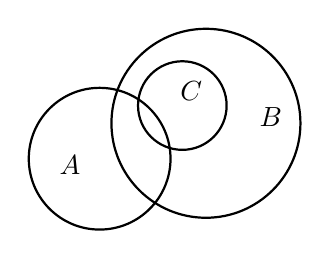
\begin{tikzpicture}[scale=0.75]
\draw[thick] (-0.8,-0.3) circle (1.2); \draw[thick] (1,0.3) circle (1.6); \draw[thick] (0.6,0.6) circle (0.75);
\node at (-1.3,-0.4) {$A$}; \node at (2.1,0.4) {$B$}; \node at (0.75,0.85) {$C$};
\end{tikzpicture}
\end{center}
\resp{a) 8;\ b) 1;\ c) 7;\ d) 3;\ e) 12.}
\end{questao}

\begin{questao}{2}{autoral}{6-H3, 6-U3}\label{u6:natacao}
Numa turma de 40 alunos, 32 fazem natação e 25 fazem judô. Qual é o menor número possível de alunos que fazem os dois esportes? E o maior?
\resp{17 e 25.}
\end{questao}

\begin{questao}{2}{adaptado de U.E. Londrina-PR via FME, ano não informado}{6-H1, 6-U2, 6-E1}\label{u6:uel20}
Um grupo de estudantes resolveu fazer uma pesquisa sobre as preferências dos alunos quanto ao cardápio do Restaurante Universitário. Nove alunos optaram somente por carne de frango, 3 somente por peixes, 7 por carne bovina e frango, 9 por peixe e carne bovina (nesses dois números estão incluídos os que optaram pelos três tipos) e 4 pelos três tipos de carne. Considerando que 20 alunos manifestaram-se vegetarianos, 36 não optaram por carne bovina e 42 não optaram por peixe, assinale a alternativa que apresenta o número de alunos entrevistados.
\begin{multicols}{5}
\begin{enumerate}[label=\alph*)]
  \item 38
  \item 42
  \item 58
  \item 62
  \item 78
\end{enumerate}
\end{multicols}
\resp{c. Só bovina e frango: 3; só peixe e bovina: 5. Fora da bovina: $9+3+\text{(só peixe e frango)}+20=36$, logo só peixe e frango $=4$. Fora do peixe: $9+\text{(só bovina)}+3+20=42$, logo só bovina $=10$. Total: $9+3+10+3+5+4+4+20=58$.}
\end{questao}

\begin{questao}{2}{FGV-SP via FME, ano não informado}{6-H2, 6-H3}\label{u6:fgv36}
Uma pesquisa de mercado sobre determinado eletrodoméstico mostrou que 37\% dos entrevistados preferem a marca X, 40\% preferem a marca Y, 30\% preferem a marca Z, 25\% preferem X e Y, 8\% preferem Y e Z, 3\% preferem X e Z e 1\% prefere as três marcas. Considerando que há os que não preferem nenhuma das três marcas, a porcentagem dos que não preferem nem X nem Y é:
\begin{multicols}{5}
\begin{enumerate}[label=\alph*)]
  \item 20\%
  \item 23\%
  \item 30\%
  \item 42\%
  \item 48\%
\end{enumerate}
\end{multicols}
\resp{e. $n(X\cup Y)=37\%+40\%-25\%=52\%$; nem X nem Y: 48\%.}
\end{questao}

\begin{questao}{2}{UF-ES via FME, ano não informado}{6-H3, 6-U2, 6-E4}\label{u6:ufes28}
Existem, nas cidades brasileiras, 18 milhões de pessoas sem abastecimento público de água potável, 93 milhões sem redes de esgotos sanitários e 14 milhões sem coleta de lixo. Admita que 103 milhões dessas pessoas carecem de pelo menos um desses serviços públicos básicos e que 6 milhões não usufruem de nenhum desses serviços. O número de pessoas, em milhões, que usufruem exatamente um desses serviços é:
\begin{multicols}{5}
\begin{enumerate}[label=\alph*)]
  \item 8
  \item 10
  \item 12
  \item 14
  \item 16
\end{enumerate}
\end{multicols}
\resp{b. Quem usufrui de exatamente um serviço carece de exatamente dois. Com $e_3=6$: $e_1+e_2+6=103$ e $e_1+2e_2+18=125$, logo $e_2=10$.}
\end{questao}

\begin{questao}{2}{UF-PE via FME, ano não informado}{6-H1, 6-H3, 6-U2}\label{u6:ufpe34}
Os alunos de uma turma cursam alguma(s) dentre as disciplinas Matemática, Física e Química. Sabendo que:
\begin{itemize}[leftmargin=1.4em,itemsep=0pt]
  \item o número de alunos que cursam Matemática e Física excede em 5 o número de alunos que cursam as três disciplinas;
  \item existem 7 alunos que cursam Matemática e Química, mas não cursam Física;
  \item existem 6 alunos que cursam Física e Química, mas não cursam Matemática;
  \item o número de alunos que cursam exatamente uma das disciplinas é 150;
  \item o número de alunos que cursam pelo menos uma das três disciplinas é 190.
\end{itemize}
Quantos alunos cursam as três disciplinas?
\resp{22.}
\end{questao}

\begin{questao}{2}{FME, exercício 57}{6-H1, 6-U4}\label{u6:fme57}
Determine os conjuntos $A$, $B$ e $C$ que satisfazem as seguintes seis condições:
\begin{multicols}{2}
\begin{enumerate}[label=\arabic*.ª)]
  \item $A\cup B\cup C=\{z,x,v,u,t,s,r,q,p\}$
  \item $A\cap B=\{r,s\}$
  \item $B\cap C=\{s,x\}$
  \item $C\cap A=\{s,t\}$
  \item $A\cup C=\{p,q,r,s,t,u,v,x\}$
  \item $A\cup B=\{p,q,r,s,t,x,z\}$
\end{enumerate}
\end{multicols}
\resp{$A=\{p,q,r,s,t\}$, $B=\{r,s,x,z\}$, $C=\{s,t,u,v,x\}$.}
\end{questao}

\begin{questao}{3}{UF-MG via FME, ano não informado}{6-H3}\label{u6:ufmg37}
Uma escola realizou uma pesquisa sobre os hábitos alimentares de seus alunos. Alguns resultados dessa pesquisa foram:
\begin{itemize}[leftmargin=1.4em,itemsep=0pt]
  \item 82\% do total de entrevistados gostam de chocolate;
  \item 78\% do total de entrevistados gostam de pizza; e
  \item 75\% do total de entrevistados gostam de batata frita.
\end{itemize}
Então, é correto afirmar que, no total de alunos entrevistados, a porcentagem dos que gostam, ao mesmo tempo, de chocolate, de pizza e de batata frita é, pelo menos, de
\begin{multicols}{4}
\begin{enumerate}[label=\alph*)]
  \item 25\%.
  \item 30\%.
  \item 35\%.
  \item 40\%.
\end{enumerate}
\end{multicols}
\resp{c.}
\end{questao}

\begin{questao}{3}{UF-ES via FME, ano não informado}{6-H1, 6-H3}\label{u6:ufes30}
Em um grupo de 93 torcedores,
\begin{itemize}[leftmargin=1.4em,itemsep=0pt]
  \item todos torcem pelo Flamengo, pelo Cruzeiro ou pelo Palmeiras;
  \item ninguém torce pelo Flamengo e pelo Cruzeiro ao mesmo tempo;
  \item exatamente 12 desses torcedores torcem por dois dos três times;
  \item o número de torcedores que torcem apenas pelo Flamengo é o dobro do número de torcedores que torcem pelo Palmeiras;
  \item pelo menos 4 torcedores torcem apenas pelo Cruzeiro.
\end{itemize}
Com base nessas informações, é correto afirmar que o número máximo possível de torcedores do Palmeiras no grupo é:
\begin{multicols}{5}
\begin{enumerate}[label=\alph*)]
  \item 27
  \item 29
  \item 31
  \item 33
  \item 35
\end{enumerate}
\end{multicols}
\resp{b.}
\end{questao}

\begin{questao}[integradora]{3}{Unicamp-SP via FME, ano não informado}{6-H1, 6-U2}\label{u6:unicamp35}
Três candidatos, A, B e C, concorrem à presidência de um clube. Uma pesquisa apontou que, dos sócios entrevistados, 150 não pretendem votar. Dentre os entrevistados que estão dispostos a participar da eleição, 40 sócios votariam apenas no candidato A, 70 votariam apenas em B e 100 votariam apenas no candidato C. Além disso, 190 disseram que não votariam em A, 110 disseram que não votariam em C e 10 sócios estão na dúvida e podem votar tanto em A como em C, mas não em B. Finalmente, a pesquisa revelou que 10 entrevistados votariam em qualquer candidato. Com base nesses dados, pergunta-se:
\begin{enumerate}[label=\alph*)]
  \item Quantos sócios entrevistados estão em dúvida entre votar em B ou em C, mas não votariam em A? Dentre os sócios consultados que pretendem participar da eleição, quantos não votariam em B?
  \item Quantos sócios participaram da pesquisa? Suponha que a pesquisa represente fielmente as intenções de voto de todos os sócios do clube. Escolhendo um sócio ao acaso, qual a probabilidade de que ele vá participar da eleição mas ainda não tenha se decidido por um único candidato?
\end{enumerate}
(Sugestão: utilize o diagrama de Venn.)
\resp{a) 20; 150;\ b) 400; $\frac{40}{400}=\frac{1}{10}$ (probabilidade = casos favoráveis $\div$ total).}
\end{questao}

\subsubsection*{Mais questões de vestibular}
Questões de vestibular sobre o assunto da unidade que ficaram fora da sequência acima, em ordem de nível. As respostas estão no fim da unidade, com as demais.

\begin{questao}{1}{U.E. Londrina-PR via FME, ano não informado}{6-H3, 6-U1}\label{u6:uel25}
Num dado momento, três canais de TV tinham, em sua programação, novelas em seus horários nobres: a novela A no canal A, a novela B no canal B e a novela C no canal C. Numa pesquisa com 3\,000 pessoas, perguntou-se quais novelas agradavam. A tabela a seguir indica o número de telespectadores que designaram as novelas como agradáveis.
\begin{center}
\small
\begin{tabular}{l|ccccccc}
Novelas & A & B & C & A e B & A e C & B e C & A, B e C\\\hline
Número de espectadores & 1\,450 & 1\,150 & 900 & 350 & 400 & 300 & 100
\end{tabular}
\end{center}
Quantos telespectadores entrevistados não acham agradável nenhuma das três novelas?
\begin{multicols}{3}
\begin{enumerate}[label=\alph*)]
  \item 300 telespectadores.
  \item 370 telespectadores.
  \item 450 telespectadores.
  \item 470 telespectadores.
  \item 500 telespectadores.
\end{enumerate}
\end{multicols}
\resp{c.}
\end{questao}

\begin{questao}{2}{UF-PA via FME, ano não informado}{6-H3}\label{u6:ufpa26}
Um professor de Matemática, ao lecionar Teoria dos Conjuntos em uma certa turma, realizou uma pesquisa sobre as preferências clubísticas de seus $n$ alunos, tendo chegado ao seguinte resultado:
\begin{itemize}[leftmargin=1.4em,itemsep=0pt]
  \item 23 alunos torcem pelo Paysandu Sport Club;
  \item 23 alunos torcem pelo Clube do Remo;
  \item 15 alunos torcem pelo Clube de Regatas Vasco da Gama;
  \item 6 alunos torcem pelo Paysandu e pelo Vasco;
  \item 5 alunos torcem pelo Vasco e pelo Remo.
\end{itemize}
Se designarmos por $A$ o conjunto dos torcedores do Paysandu, por $B$ o conjunto dos torcedores do Remo e por $C$ o conjunto dos torcedores do Vasco, todos da referida turma, teremos, evidentemente, $A\cap B=\varnothing$. Concluímos que o número $n$ de alunos desta turma é
\begin{multicols}{5}
\begin{enumerate}[label=\alph*)]
  \item 49.
  \item 50.
  \item 47.
  \item 45.
  \item 46.
\end{enumerate}
\end{multicols}
\resp{b. Como $A\cap B=\varnothing$, também $A\cap B\cap C=\varnothing$: $23+23+15-6-5=50$ (supondo, como o enunciado sugere, que todos torcem por algum dos três).}
\end{questao}

\begin{questao}{2}{UF-PE via FME, ano não informado}{6-H3}\label{u6:ufpe31}
Em uma pesquisa com os 60 alunos de uma turma do ensino médio sobre a preferência deles com respeito às disciplinas Matemática, Física e Química, foi constatado que:
\begin{itemize}[leftmargin=1.4em,itemsep=0pt]
  \item 14 alunos gostam de exatamente duas das três disciplinas;
  \item 20 alunos gostam das três disciplinas;
  \item 10 alunos não gostam de nenhuma das três disciplinas.
\end{itemize}
Quantos alunos gostam de exatamente uma das três disciplinas?
\begin{multicols}{5}
\begin{enumerate}[label=\alph*)]
  \item 18
  \item 17
  \item 16
  \item 15
  \item 14
\end{enumerate}
\end{multicols}
\resp{c.}
\end{questao}

\begin{questao}{2}{Udesc-SC via FME, ano não informado}{6-H1, 6-H2}\label{u6:udesc22}
\textbf{O que os brasileiros andam lendo?} O brasileiro lê, em média, 4,7 livros por ano. Este é um dos principais resultados da pesquisa \emph{Retratos da Leitura no Brasil}, encomendada pelo Instituto Pró-Livro ao Ibope Inteligência, que também pesquisou o comportamento do leitor brasileiro, as preferências e as motivações dos leitores, bem como os canais e a forma de acesso aos livros. (Fonte: Associação Brasileira de Encadernação e Restauro, adapt.)

Supõe-se que em uma pesquisa envolvendo 660 pessoas, cujo objetivo era verificar o que elas estão lendo, obtiveram-se os seguintes resultados: 100 pessoas leem somente revistas, 300 pessoas leem somente livros e 150 pessoas leem somente jornais. Supõe-se ainda que, dessas 660 pessoas, 80 leem livros e revistas, 50 leem jornais e revistas, 60 leem livros e jornais e 40 leem revistas, jornais e livros. Em relação ao resultado dessa pesquisa, são feitas as seguintes afirmações:
\begin{enumerate}[label=\Roman*.]
  \item Apenas 40 pessoas leem pelo menos um dos três meios de comunicação citados.
  \item Quarenta pessoas leem somente revistas e livros, e não leem jornais.
  \item Apenas 440 pessoas leem revistas ou livros.
\end{enumerate}
Assinale a alternativa correta.
\begin{enumerate}[label=\alph*)]
  \item Somente as afirmativas I e III são verdadeiras.
  \item Somente as afirmativas I e II são verdadeiras.
  \item Somente as afirmativas I, II e III são verdadeiras.
  \item Somente a afirmativa II é verdadeira.
  \item Somente a afirmativa I é verdadeira.
\end{enumerate}
\resp{d.}
\end{questao}

\begin{questao}{2}{UF-PI via FME, ano não informado}{6-H2, 6-H3}\label{u6:ufpi27}
O diretor de uma tradicional escola da cidade de Teresina resolveu fazer uma pesquisa de opinião junto aos seus 590 alunos do Ensino Médio sobre as políticas públicas de acesso ao Ensino Superior. No questionário, perguntava-se sobre a aprovação de: Cotas, Bolsas e Enem, como modelo de exame vestibular. As respostas dos alunos foram sintetizadas na tabela abaixo:
\begin{center}
\small
\begin{tabular}{l|ccccccc}
Política pública & Cotas & Bolsas & Enem & \begin{tabular}[c]{@{}c@{}}Cotas e\\Bolsas\end{tabular} & \begin{tabular}[c]{@{}c@{}}Bolsas e\\Enem\end{tabular} & \begin{tabular}[c]{@{}c@{}}Cotas e\\Enem\end{tabular} & \begin{tabular}[c]{@{}c@{}}Cotas, Bolsas\\e Enem\end{tabular}\\\hline
Número de aprovações & 226 & 147 & 418 & 53 & 85 & 116 & 44
\end{tabular}
\end{center}
Sobre a pesquisa e a tabela anterior, é correto afirmar que
\begin{enumerate}[label=\alph*)]
  \item a quantidade de alunos que não opinaram por nenhuma das três políticas é 12.
  \item a quantidade de alunos que aprovam apenas uma política pública é 415.
  \item a quantidade de alunos que aprovam mais de uma política é 167.
  \item a quantidade de alunos que aprovam as três políticas é 45.
  \item há mais alunos que aprovam cotas do que alunos que aprovam somente o Enem.
\end{enumerate}
\resp{b.}
\end{questao}

\begin{questao}{2}{adaptado de U.F. Uberlândia-MG via FME, ano não informado}{6-H1, 6-U2, 6-E1}\label{u6:ufu33}
De uma escola de Uberlândia, partiu uma excursão para Caldas Novas com 40 alunos. Ao chegar em Caldas Novas, 2 alunos adoeceram e não frequentaram as piscinas. Todos os demais alunos frequentaram as piscinas, sendo 20 pela manhã e à tarde (incluídos os que foram também à noite), 12 somente pela manhã, 3 somente à noite e 8 pela manhã, à tarde e à noite. Se ninguém frequentou as piscinas somente no período da tarde, quantos alunos frequentaram as piscinas à noite?
\begin{multicols}{4}
\begin{enumerate}[label=\alph*)]
  \item 16
  \item 12
  \item 14
  \item 18
\end{enumerate}
\end{multicols}
\resp{c.}
\end{questao}

\begin{questao}{3}{UF-PE via FME, ano não informado}{6-H1}\label{u6:ufpe19}
Os 200 estudantes de uma escola que praticam esportes escolhem duas dentre as modalidades seguintes: futebol, handebol, basquete e futebol de salão. Entretanto, nenhum estudante da escola escolheu futebol e basquete ou handebol e futebol de salão. Sabendo que 65\% dos alunos escolheram futebol, 60\% escolheram futebol de salão, 35\% escolheram basquete e 25\% dos jogadores de handebol também jogam basquete, quantos são os alunos da escola que jogam futebol e futebol de salão?
\resp{70.}
\end{questao}

\begin{sintese}
\textbf{Ao fim desta unidade, você deveria saber:}
\begin{itemize}[leftmargin=1.4em,itemsep=1pt]
  \item desenhar as oito regiões de três conjuntos e preenchê-las de dentro para fora;
  \item calcular $n(A\cup B\cup C)$ e explicar por que os que estão nos três são devolvidos;
  \item distinguir \enquote{$A$ e $B$} de \enquote{só $A$ e $B$}, e \enquote{exatamente dois} de \enquote{pelo menos dois};
  \item transformar dados indiretos em equações nas regiões;
  \item achar o menor e o maior valor que os dados permitem, exigindo que nenhuma região seja negativa;
  \item determinar conjuntos elemento a elemento.
\end{itemize}
\smallskip\noindent\textbf{Responda com suas palavras, sem consultar.} Depois, confira com a caixa \emph{Para lembrar} (p.~\pageref{lembrar-u6}) e com a seção indicada.
\begin{enumerate}[label=\arabic*.,leftmargin=1.4em]
  \perguntasintese{Por que se desenham as oito regiões, mesmo as que podem estar vazias? \ondever{construção 6-H1}}
  \perguntasintese{Por que, na fórmula de três conjuntos, a interseção dos três é somada de volta? \ondever{construção 6-H3}}
  \perguntasintese{Num enunciado, como você reconhece que os dados só limitam a resposta, e o que faz então? \ondever{Onde é usado?}}
  \perguntasintese{Qual erro você cometeria ao escrever o número de \enquote{$A$ e $B$} direto na região só $A$ e $B$? Como evitá-lo? \ondever{Erros comuns}}
\end{enumerate}
\end{sintese}

% ------------------------------------------------------------
\Respostas
{\small\resposta{S}{Síntese de domínio: confira com a caixa \emph{Para lembrar} (p.~\pageref{lembrar-u6}) e com a seção indicada em cada pergunta.}}


% %% FIM UNIDADES %%
\clearpage
% Glossário do capítulo — no FIM do capítulo, como consulta (didática v3 §5).
% Montado no fechamento a partir dos termos que cada unidade define (dossiê §1 "termos novos").
% Uma linha por termo + a unidade onde é construído.
\section*{Glossário do capítulo}
\addcontentsline{toc}{section}{Glossário do capítulo}
\markright{Glossário}
{\small Termos e símbolos usados no capítulo, com o significado em uma linha e a unidade onde são construídos.}

\subsection*{Termos}
\begin{glossario}
\item[Termo] Significado em uma linha. \hfill\emph{Unid.~1}
\end{glossario}

\subsection*{Símbolos}
\begin{center}\small
\begin{tabular}{clll}\toprule
\sffamily\bfseries Símbolo & \sffamily\bfseries Leitura & \sffamily\bfseries Exemplo & \sffamily\bfseries Unid.\\\midrule
$x$ & leitura & exemplo & 1\\\bottomrule
\end{tabular}
\end{center}


\backmatter
% Fontes do capítulo: uma entrada por chave \src{…}. Ordem = ordem de primeira citação (aproximada).
% Fonte primária ao lado da secundária frágil sempre que localizada (A5, E-R3-5).
% Formato: Autor, \emph{Obra}, local (trad./ed.). \url{…}  ·  artigos com DOI.
\chapter*{Fontes}
\addcontentsline{toc}{chapter}{Fontes}
\markboth{Fontes}{Fontes}
\small
Os números sobrescritos no texto remetem a esta lista. As questões trazem a procedência no próprio cabeçalho. Os endereços da web foram acessados em novembro de 2026, e em todas as páginas da web (Wikipédia, enciclopédias e repositórios) vale a versão dessa data. Quando a fonte acessível é secundária, a obra original vem citada ao lado, sempre que localizada.

\begingroup
\makeatletter
% a lista entra logo abaixo do título "Fontes": sem novo capítulo nem cabeçalho "Referências"
\renewcommand{\chapter}{\@ifstar{\@gobble}{\@gobble}}
\renewcommand{\@mkboth}[2]{}
\makeatother
\begin{thebibliography}{999}\setlength{\itemsep}{0.2em}
\bibitem{fme} G.~Iezzi et al., \emph{Fundamentos de Matemática Elementar}, vol.~1, cap.~II, \enquote{Conjuntos}. São Paulo: Atual.
\end{thebibliography}
\endgroup

\end{document}
